
%% bare_jrnl_transmag.tex   
%% V1.4b
%% 2015/08/26
%% by Michael Shell
%% see http://www.michaelshell.org/
%% for current contact information.
%%
%% This is a skeleton file demonstrating the use of IEEEtran.cls
%% (requires IEEEtran.cls version 1.8b or later) with an IEEE
%% Transactions on Magnetics journal paper.
%%
%% Support sites:
%% http://www.michaelshell.org/tex/ieeetran/
%% http://www.ctan.org/pkg/ieeetran
%% and
%% http://www.ieee.org/

%%*************************************************************************
%% Legal Notice:
%% This code is offered as-is without any warranty either expressed or
%% implied; without even the implied warranty of MERCHANTABILITY or
%% FITNESS FOR A PARTICULAR PURPOSE!
%% User assumes all risk.
%% In no event shall the IEEE or any contributor to this code be liable for
%% any damages or losses, including, but not limited to, incidental,
%% consequential, or any other damages, resulting from the use or misuse
%% of any information contained here.
%%
%% All comments are the opinions of their respective authors and are not
%% necessarily endorsed by the IEEE.
%%
%% This work is distributed under the LaTeX Project Public License (LPPL)
%% ( http://www.latex-project.org/ ) version 1.3, and may be freely used,
%% distributed and modified. A copy of the LPPL, version 1.3, is included
%% in the base LaTeX documentation of all distributions of LaTeX released
%% 2003/12/01 or later.
%% Retain all contribution notices and credits.
%% ** Modified files should be clearly indicated as such, including  **
%% ** renaming them and changing author support contact information. **
%%*************************************************************************


% *** Authors should verify (and, if needed, correct) their LaTeX system  ***
% *** with the testflow diagnostic prior to trusting their LaTeX platform ***
% *** with production work. The IEEE's font choices and paper sizes can   ***
% *** trigger bugs that do not appear when using other class files.       ***                          ***
% The testflow support page is at:
% http://www.michaelshell.org/tex/testflow/



\documentclass[journal,transmag]{IEEEtran}
%
% If IEEEtran.cls has not been installed into the LaTeX system files,
% manually specify the path to it like:
% \documentclass[journal]{../sty/IEEEtran}





% Some very useful LaTeX packages include:
% (uncomment the ones you want to load)


% *** MISC UTILITY PACKAGES ***
%
%\usepackage{ifpdf}
% Heiko Oberdiek's ifpdf.sty is very useful if you need conditional
% compilation based on whether the output is pdf or dvi.
% usage:
% \ifpdf
%   % pdf code
% \else
%   % dvi code
% \fi
% The latest version of ifpdf.sty can be obtained from:
% http://www.ctan.org/pkg/ifpdf
% Also, note that IEEEtran.cls V1.7 and later provides a builtin
% \ifCLASSINFOpdf conditional that works the same way.
% When switching from latex to pdflatex and vice-versa, the compiler may
% have to be run twice to clear warning/error messages.






% *** CITATION PACKAGES ***
%
%\usepackage{cite}
% cite.sty was written by Donald Arseneau
% V1.6 and later of IEEEtran pre-defines the format of the cite.sty package
% \cite{} output to follow that of the IEEE. Loading the cite package will
% result in citation numbers being automatically sorted and properly
% "compressed/ranged". e.g., [1], [9], [2], [7], [5], [6] without using
% cite.sty will become [1], [2], [5]--[7], [9] using cite.sty. cite.sty's
% \cite will automatically add leading space, if needed. Use cite.sty's
% noadjust option (cite.sty V3.8 and later) if you want to turn this off
% such as if a citation ever needs to be enclosed in parenthesis.
% cite.sty is already installed on most LaTeX systems. Be sure and use
% version 5.0 (2009-03-20) and later if using hyperref.sty.
% The latest version can be obtained at:
% http://www.ctan.org/pkg/cite
% The documentation is contained in the cite.sty file itself.






% *** GRAPHICS RELATED PACKAGES ***
%
\ifCLASSINFOpdf
  %\usepackage[pdftex]{graphicx}
  % declare the path(s) where your graphic files are
  % \graphicspath{{../pdf/}{../jpeg/}}
  % and their extensions so you won't have to specify these with
  % every instance of \includegraphics
  % \DeclareGraphicsExtensions{.pdf,.jpeg,.png}
\else
  % or other class option (dvipsone, dvipdf, if not using dvips). graphicx
  % will default to the driver specified in the system graphics.cfg if no
  % driver is specified.
  % \usepackage[dvips]{graphicx}
  % declare the path(s) where your graphic files are
  % \graphicspath{{../eps/}}
  % and their extensions so you won't have to specify these with
  % every instance of \includegraphics
  % \DeclareGraphicsExtensions{.eps}
\fi
% graphicx was written by David Carlisle and Sebastian Rahtz. It is
% required if you want graphics, photos, etc. graphicx.sty is already
% installed on most LaTeX systems. The latest version and documentation
% can be obtained at:
% http://www.ctan.org/pkg/graphicx
% Another good source of documentation is "Using Imported Graphics in
% LaTeX2e" by Keith Reckdahl which can be found at:
% http://www.ctan.org/pkg/epslatex
%
% latex, and pdflatex in dvi mode, support graphics in encapsulated
% postscript (.eps) format. pdflatex in pdf mode supports graphics
% in .pdf, .jpeg, .png and .mps (metapost) formats. Users should ensure
% that all non-photo figures use a vector format (.eps, .pdf, .mps) and
% not a bitmapped formats (.jpeg, .png). The IEEE frowns on bitmapped formats
% which can result in "jaggedy"/blurry rendering of lines and letters as
% well as large increases in file sizes.
%
% You can find documentation about the pdfTeX application at:
% http://www.tug.org/applications/pdftex




% *** MATH PACKAGES ***
%
%\usepackage{amsmath}
% A popular package from the American Mathematical Society that provides
% many useful and powerful commands for dealing with mathematics.
%
% Note that the amsmath package sets \interdisplaylinepenalty to 10000
% thus preventing page breaks from occurring within multiline equations. Use:
%\interdisplaylinepenalty=2500
% after loading amsmath to restore such page breaks as IEEEtran.cls normally
% does. amsmath.sty is already installed on most LaTeX systems. The latest
% version and documentation can be obtained at:
% http://www.ctan.org/pkg/amsmath





% *** SPECIALIZED LIST PACKAGES ***
%
%\usepackage{algorithmic}
% algorithmic.sty was written by Peter Williams and Rogerio Brito.
% This package provides an algorithmic environment fo describing algorithms.
% You can use the algorithmic environment in-text or within a figure
% environment to provide for a floating algorithm. Do NOT use the algorithm
% floating environment provided by algorithm.sty (by the same authors) or
% algorithm2e.sty (by Christophe Fiorio) as the IEEE does not use dedicated
% algorithm float types and packages that provide these will not provide
% correct IEEE style captions. The latest version and documentation of
% algorithmic.sty can be obtained at:
% http://www.ctan.org/pkg/algorithms
% Also of interest may be the (relatively newer and more customizable)
% algorithmicx.sty package by Szasz Janos:
% http://www.ctan.org/pkg/algorithmicx




% *** ALIGNMENT PACKAGES ***
%
%\usepackage{array}
% Frank Mittelbach's and David Carlisle's array.sty patches and improves
% the standard LaTeX2e array and tabular environments to provide better
% appearance and additional user controls. As the default LaTeX2e table
% generation code is lacking to the point of almost being broken with
% respect to the quality of the end results, all users are strongly
% advised to use an enhanced (at the very least that provided by array.sty)
% set of table tools. array.sty is already installed on most systems. The
% latest version and documentation can be obtained at:
% http://www.ctan.org/pkg/array


% IEEEtran contains the IEEEeqnarray family of commands that can be used to
% generate multiline equations as well as matrices, tables, etc., of high
% quality.




% *** SUBFIGURE PACKAGES ***
%\ifCLASSOPTIONcompsoc
%  \usepackage[caption=false,font=normalsize,labelfont=sf,textfont=sf]{subfig}
%\else
%  \usepackage[caption=false,font=footnotesize]{subfig}
%\fi
% subfig.sty, written by Steven Douglas Cochran, is the modern replacement
% for subfigure.sty, the latter of which is no longer maintained and is
% incompatible with some LaTeX packages including fixltx2e. However,
% subfig.sty requires and automatically loads Axel Sommerfeldt's caption.sty
% which will override IEEEtran.cls' handling of captions and this will result
% in non-IEEE style figure/table captions. To prevent this problem, be sure
% and invoke subfig.sty's "caption=false" package option (available since
% subfig.sty version 1.3, 2005/06/28) as this is will preserve IEEEtran.cls
% handling of captions.
% Note that the Computer Society format requires a larger sans serif font
% than the serif footnote size font used in traditional IEEE formatting
% and thus the need to invoke different subfig.sty package options depending
% on whether compsoc mode has been enabled.
%
% The latest version and documentation of subfig.sty can be obtained at:
% http://www.ctan.org/pkg/subfig



% *** FLOAT PACKAGES ***
%
%\usepackage{fixltx2e}
% fixltx2e, the successor to the earlier fix2col.sty, was written by
% Frank Mittelbach and David Carlisle. This package corrects a few problems
% in the LaTeX2e kernel, the most notable of which is that in current
% LaTeX2e releases, the ordering of single and double column floats is not
% guaranteed to be preserved. Thus, an unpatched LaTeX2e can allow a
% single column figure to be placed prior to an earlier double column
% figure.
% Be aware that LaTeX2e kernels dated 2015 and later have fixltx2e.sty's
% corrections already built into the system in which case a warning will
% be issued if an attempt is made to load fixltx2e.sty as it is no longer
% needed.
% The latest version and documentation can be found at:
% http://www.ctan.org/pkg/fixltx2e


%\usepackage{stfloats}
% stfloats.sty was written by Sigitas Tolusis. This package gives LaTeX2e
% the ability to do double column floats at the bottom of the page as well
% as the top. (e.g., "\begin{figure*}[!b]" is not normally possible in
% LaTeX2e). It also provides a command:
%\fnbelowfloat
% to enable the placement of footnotes below bottom floats (the standard
% LaTeX2e kernel puts them above bottom floats). This is an invasive package
% which rewrites many portions of the LaTeX2e float routines. It may not work
% with other packages that modify the LaTeX2e float routines. The latest
% version and documentation can be obtained at:
% http://www.ctan.org/pkg/stfloats
% Do not use the stfloats baselinefloat ability as the IEEE does not allow
% \baselineskip to stretch. Authors submitting work to the IEEE should note
% that the IEEE rarely uses double column equations and that authors should try
% to avoid such use. Do not be tempted to use the cuted.sty or midfloat.sty
% packages (also by Sigitas Tolusis) as the IEEE does not format its papers in
% such ways.
% Do not attempt to use stfloats with fixltx2e as they are incompatible.
% Instead, use Morten Hogholm'a dblfloatfix which combines the features
% of both fixltx2e and stfloats:
%
% \usepackage{dblfloatfix}
% The latest version can be found at:
% http://www.ctan.org/pkg/dblfloatfix




%\ifCLASSOPTIONcaptionsoff
%  \usepackage[nomarkers]{endfloat}
% \let\MYoriglatexcaption\caption
% \renewcommand{\caption}[2][\relax]{\MYoriglatexcaption[#2]{#2}}
%\fi
% endfloat.sty was written by James Darrell McCauley, Jeff Goldberg and
% Axel Sommerfeldt. This package may be useful when used in conjunction with
% IEEEtran.cls'  captionsoff option. Some IEEE journals/societies require that
% submissions have lists of figures/tables at the end of the paper and that
% figures/tables without any captions are placed on a page by themselves at
% the end of the document. If needed, the draftcls IEEEtran class option or
% \CLASSINPUTbaselinestretch interface can be used to increase the line
% spacing as well. Be sure and use the nomarkers option of endfloat to
% prevent endfloat from "marking" where the figures would have been placed
% in the text. The two hack lines of code above are a slight modification of
% that suggested by in the endfloat docs (section 8.4.1) to ensure that
% the full captions always appear in the list of figures/tables - even if
% the user used the short optional argument of \caption[]{}.
% IEEE papers do not typically make use of \caption[]'s optional argument,
% so this should not be an issue. A similar trick can be used to disable
% captions of packages such as subfig.sty that lack options to turn off
% the subcaptions:
% For subfig.sty:
% \let\MYorigsubfloat\subfloat
% \renewcommand{\subfloat}[2][\relax]{\MYorigsubfloat[]{#2}}
% However, the above trick will not work if both optional arguments of
% the \subfloat command are used. Furthermore, there needs to be a
% description of each subfigure *somewhere* and endfloat does not add
% subfigure captions to its list of figures. Thus, the best approach is to
% avoid the use of subfigure captions (many IEEE journals avoid them anyway)
% and instead reference/explain all the subfigures within the main caption.
% The latest version of endfloat.sty and its documentation can obtained at:
% http://www.ctan.org/pkg/endfloat
%
% The IEEEtran \ifCLASSOPTIONcaptionsoff conditional can also be used
% later in the document, say, to conditionally put the References on a
% page by themselves.




% *** PDF, URL AND HYPERLINK PACKAGES ***
%
%\usepackage{url}
% url.sty was written by Donald Arseneau. It provides better support for
% handling and breaking URLs. url.sty is already installed on most LaTeX
% systems. The latest version and documentation can be obtained at:
% http://www.ctan.org/pkg/url
% Basically, \url{my_url_here}.




% *** Do not adjust lengths that control margins, column widths, etc. ***
% *** Do not use packages that alter fonts (such as pslatex).         ***
% There should be no need to do such things with IEEEtran.cls V1.6 and later.
% (Unless specifically asked to do so by the journal or conference you plan
% to submit to, of course. )


% correct bad hyphenation here
\usepackage{booktabs} % For formal tables
\usepackage{indentfirst} % For formal tables\cite{}
\usepackage{url} % For formal tables
\usepackage{graphicx}
\usepackage{balance}  % for  \balance command ON LAST PAGE  (only there!)
\usepackage{caption}
\usepackage{subfig}
\usepackage{amsmath}
\usepackage{amssymb}
\usepackage{algorithm}
%\usepackage{algorithmic}
\usepackage{color}
\usepackage{comment}
\usepackage{flushend}
\usepackage{bm}
\usepackage{algpseudocode}
\usepackage{amsthm}
\renewcommand{\algorithmicrequire}{\textbf{Input:}}
\renewcommand{\algorithmicensure}{\textbf{Output:}}
\newtheorem{theorem}{Theorem}
\hyphenation{op-tical net-works semi-conduc-tor}


\begin{document}

\title{bHash: An I/O Efficient External Hash Grouping Scheme}
%\IEEEauthorrefmark{2}
\author{\IEEEauthorblockN{Xiaowang Kong, Yanfeng Zhang, Ge Yu}
Northeastern University, Liaoning, 110819, China
\IEEEauthorblockN{kongxiaowang@126.com, zhangyf@cc.neu.edu.cn, yuge@mail.neu.edu.cn}
%Montgomery Scott\IEEEauthorrefmark{3}, and
%Eldon Tyrell\IEEEauthorrefmark{4},~\IEEEmembership{Fellow,~IEEE}}
%\IEEEauthorblockA{\IEEEauthorrefmark{1}School of Computer Science and Engineering,
%Northeastern University, ShenYang, 110819, China}
%\IEEEauthorblockA{\IEEEauthorrefmark{1}kongxiaowang@126.com}
%\IEEEauthorblockA{\IEEEauthorrefmark{2}zhangyf@cc.neu.edu.cn}
%\IEEEauthorblockA{\IEEEauthorrefmark{3}yuge@mail.neu.edu.cn}
}% <-this % stops an unwanted space
%\thanks{Manuscript received December 1, 2012; revised August 26, 2015.
%Corresponding author: M. Shell (email: http://www.michaelshell.org/contact.html).}}


% The paper headers
%������������ע�͵���
%\markboth{Journal of \LaTeX\ Class Files,~Vol.~14, No.~8, August~2015}%
%{Shell \MakeLowercase{\textit{et al.}}: Bare Demo of IEEEtran.cls for IEEE Transactions on Magnetics Journals}
%������������ע�͵���
% The only time the second header will appear is for the odd numbered pages
% after the title page when using the twoside option.
%
% *** Note that you probably will NOT want to include the author's ***
% *** name in the headers of peer review papers.                   ***
% You can use \ifCLASSOPTIONpeerreview for conditional compilation here if
% you desire.
% If you want to put a publisher's ID mark on the page you can do it like
% this:
%\IEEEpubid{0000--0000/00\$00.00~\copyright~2015 IEEE}
% Remember, if you use this you must call \IEEEpubidadjcol in the second
% column for its text to clear the IEEEpubid mark.



% use for special paper notices
%\IEEEspecialpapernotice{(Invited Paper)}


% for Transactions on Magnetics papers, we must declare the abstract and
% index terms PRIOR to the title within the \IEEEtitleabstractindextext
% IEEEtran command as these need to go into the title area created by
% \maketitle.
% As a general rule, do not put math, special symbols or citations
% in the abstract or keywords.
\IEEEtitleabstractindextext{%
\begin{abstract}
We study the GroupBy implementation found in MapReduce and databases. GroupBy operation partitions a set of records into groups according to some key. Despite its  wide range of applications, most existing GroupBy implementations become very inefficient when the input data are too large to be hold in main memory. We propose an I/O efficient GroupBy implementation \emph{bHash} by exploring intelligent hash function and buffer design. bHash is a two-phase algorithm, which contains a statistics collection phase and a file filling phase. The first phase generates an offset table for each group by one pass of input. The second phase exploits an output buffer to efficiently fill the output file in terms of the offset table. We test bHash on both real-world and synthetic data sets. Compared to traditional grouping algorithms, bHash reduces redundant computation overhead significantly and especially achieves nearly-perfect performance for the skewed data. Given the same memory resource budget, bHash improves merge-sort grouping by 20\%-57.8\% and improves memory-constraint hash grouping by 45\% on execution time. bHash even performs better for skewed distributed data.


%It is used in a variety of applications such as machine learning, data mining and SQL Group By querying. However, when the input data are too large to fit into the main memory even skewed, most existing grouping algorithms become very inefficient. We introduce an external Hash Grouping Scheme by exploring Group-Size Buffer (bHash), a new key grouping scheme that adapts the combine of two classical phases: Statistics Collection and File Filling. In so doing, it achieves better grouping speed than \emph{merge-sort} and \emph{memory-constraint hash} while being more scalable than \emph{memory-constraint hash}.



%This result translates into an improvement of up to from 20\% to 57.8\% compared to \emph{merge-sort} in execution time and up to 45\% in speed compared to \emph{memory-constraint hash} algorithm when allocated the same amount of memory. For the long-tailed distributions such as Pareto, our algorithm even achieves 50\% better overall performance than \emph{merge-sort} but occupies 40\% times less memory and 45\% faster than \emph{memory-constraint hash} with 39\% times less memory.

\end{abstract}

% Note that keywords are not normally used for peerreview papers.
\begin{IEEEkeywords}
distributed computing, key value grouping, SQL database, Group By.
\end{IEEEkeywords}}



% make the title area
\maketitle


% To allow for easy dual compilation without having to reenter the
% abstract/keywords data, the \IEEEtitleabstractindextext text will
% not be used in maketitle, but will appear (i.e., to be "transported")
% here as \IEEEdisplaynontitleabstractindextext when the compsoc
% or transmag modes are not selected <OR> if conference mode is selected
% - because all conference papers position the abstract like regular
% papers do.
\IEEEdisplaynontitleabstractindextext
% \IEEEdisplaynontitleabstractindextext has no effect when using
% compsoc or transmag under a non-conference mode.







% For peer review papers, you can put extra information on the cover
% page as needed:
% \ifCLASSOPTIONpeerreview
% \begin{center} \bfseries EDICS Category: 3-BBND \end{center}
% \fi
%
% For peerreview papers, this IEEEtran command inserts a page break and
% creates the second title. It will be ignored for other modes.
\IEEEpeerreviewmaketitle


\section{Introduction}

Key value grouping operation, known as GROUP BY clause, is a key operation in database systems \cite{gray1997data}, \cite{stephens2005oracle}, \cite{mysql2009mysql}, \cite{momjian2001postgresql}. It groups a set of out-of-order records into multiple groups according to a certain key. GroupBy operation is often used with aggregate functions which produces a single row of summary information for each group, e.g., GroupBy-Aggregate in SQL. GroupBy is also widely used in distributed computing frameworks for distributing and locating the data. MapReduce \cite{dean2008mapreduce} expresses the computational process as three phases: Map, Shuffle and Reduce. During the shuffle phase, the key-value pairs that have the same key are aggregated together to form a Map output file, and they are sent to the same Reduce processor where the final cluster-wide aggregation (reduction) is applied on them. The efficiency of the key-value grouping step is crucial to both relational databases and distributed computing systems.


%Another popular use case for key grouping is to accumulate state across the stream in distributed stream processing engines (DSPEs) such as Storm \cite{storm2013storm}, S4 \cite{neumeyer2010s4}, Smaza \cite{noghabi2017samza}. This grouping in DSPEs is usually implemented by partitioning the stream on a key \cite{nasir2015power}. The strategies that are used to route tuples in a stream toward available operators can be divided into two categories: key grouping for stateful operators where a stream of tuples is partitioned in several disjoint sub-streams depending on the values contained \cite{rivetti2015efficient} and shuffle grouping for stateless operators where each tuple of a stream can be randomly assigned to any available operator \cite{Rivetti2016Online}. However, all the above works are focused on how to route kv-pairs to available operators for alleviating load imbalance but ignoring local key value aggregation overhead at the receiver side. In fact, the execution time depends on not only stream partition but also local aggregation. Our work will focus on accelerating the local GroupBy aggregation in this paper.

There are two categories of GroupBy implementations in general, sort-based grouping and hash-based grouping. Basically, the \emph{sort-based grouping} makes the data records sorted in the order of the group key, so that the records with the same group key are located together. While the \emph{hash-based grouping} typically hashes key-value pairs to a hash table structure where multiple key-value pairs in the same group (sharing the same group key) are stored in the same bucket.

Recall that key-value pairs (kv-pairs) grouping operation is the key operation in Hadoop MapReduce \cite{dean2008mapreduce}. The map output kv-pairs are locally grouped by keys before they are shuffled to reduce workers. These map output kv-pairs (i.e., reduce input kv-pairs) from various map workers are further merged to obtain a global grouped kv-pairs. Each group of kv-pairs sharing the same key is the input of a reduce function. In Hadoop Mapreduce implementation, a kind of sort-based grouping, \emph{merge-sort grouping}, is used, which can perform quite general grouping tasks at scale even in the absence of available memory. However, merge-sort grouping involves large amount of redundant computation and I/Os. The previous work \cite{shvachko2010hadoop,yu2009distributed,Li2011A} shows that merge-sort grouping adopted by Hadoop is found to be among the worst-performing choices.

For many applications, hash-based grouping is adopted because these applications require only unsorted grouping \cite{lin2011tenzing}, \cite{yu2009distributed}. However, hash-based grouping consumes more memory than sort-based grouping because it requires to load all records into memory. The performance heavily depends on the amount of available memory. A variant of hash grouping has been used in MariaDB \cite{bartholomew2012mariadb}, Oracle \cite{stephens2005oracle}, Postgresql \cite{momjian2001postgresql}, and SQL Server \cite{agrawal2005database}. It creates an in-memory hash table for grouping rows. If the hash table becomes too large to be fit in memory, the input records are partitioned into smaller work tables which are recursively partitioned until they fit into memory. Once all input groups have been processed, the completed in-memory groups are output and repeat the algorithm by reading back and aggregating one spilled partition at a time until all partitions have been processed. We refer to this approach as \emph{memory-constraint hash grouping}. It excels at efficiently aggregating large data sets and performs better than merge-sort grouping in some situations.

An alternate of hash grouping that can avoid memory overflow is using rehashing. The first hash grouping is applied to obtain coarse-grain kv-pair groups, where each group of kv-pairs covering multiple unique keys is written to a disk file. The second phase loads each kv-pairs file into memory and performs hash grouping on keys, so that the kv-pairs sharing the same key are grouped together in a bucket. These grouped kv-pairs are then written out for recycling memory to group next coarse-grain grouped kv-pairs (in next file). The number of files (coarse-grain groups) can be tuned according to available memory, and further optimizations can be applied to avoid memory overflow when processing each coarse-grain group. We refer to this approach as \emph{Partitioned hash grouping}.

In sort-based grouping, the output file position of each group is determined before the grouping starts. In hash-based grouping, the query of a specific group can be very fast. We can use an \emph{indexing-filling} approach that utilizes the advantages from both sort grouping and hash grouping. It first reads all data in one pass and evaluate the group size information associated for each key, which is maintained in an in-memory table. The output offsets of all groups can be then calculated. In other words, the output kv-pairs are indexed in the first indexing phase. The data are parsed for the second time, and the kv-pairs are written out to specific file positions according to the offset table, which is the filling phase.

In this paper, we proposed a grouping method called \emph{indexing and filling}, it is a file filling process according to an index. Indexing and filling method creates an in-memory offset index which records each group's output position in result file firstly, then writes the kv-pairs to the certain position in the result file on the basis of the offset index. In the whole process, a large amount of time is spent on seek operations during the file filling, this is mainly due to the fact that the writing of kv-pairs is not necessarily sequential, but its memory usage is very small, only an offset index is kept in memory.

As known, in real life, the group sizes in many data sets follow power-law distributions \cite{MEJPower}, the big group sizes and small group sizes vary over an enormous range. When these data sets are processed by memory-constrain hash grouping in limited memory, the sub-tables sizes are not balanced caused by big groups, which leads to multiple recursive partitions and downgrade grouping performance. The performance reduction resulting from power-law distributions often occurs in various applications, we observe that these implementations exhibit different performance and memory usage for big groups and small groups. As shown in Figure \ref{fig:paretoBig}, the \emph{indexing and filling} method performs best compared with merge-sort and memory-constraint hash grouping when grouping the big groups. Indexing and filling method proposed in this article is a file filling process according to an index, it creates an in-memory offset index which records each group's output position in result file firstly and fills the result file on the basis of the offset index, so the best grouping approach is indexing and filling for big groups. As shown in Figure \ref{fig:paretoSmall}, the \emph{partitioned hash grouping} method runs faster in limited memory when grouping small groups, that the kv-pairs in small groups are processed partition by partition is refered as partitioned hash grouping, so grouping small groups by partitioned hash is the best choice. Therefore, the ideal implementation should take the group size into account, and a hybrid grouping approach is desired.

\begin{figure}[htbp]%figure 2
\subfloat[Performance comparison on big groups]{\includegraphics[width = 1.68in]{fig/paretoBig.eps}\label{fig:paretoBig}}
    \hspace{0.23cm}
    \subfloat[Performance comparison on small groups]{\includegraphics[width =1.68in]{fig/paretoSmall.eps}\label{fig:paretoSmall}}\\
%\includegraphics[width=.5\textwidth]{fig/pareto_index_hash}
\caption{Performance comparison of big groups and small groups. The big groups and small groups are selected from a simulation data set Pareto, the group sizes of Pareto follow a power-law distribution.}
\label{fig: big and small}
\end{figure}


Based on this observation, we propose an I/O efficient hash grouping scheme \emph{power-law hash} that leverages power-law distributions and hashing in this paper, the big groups and small groups are processed separately in the algorithm, they are grouped by indexing-filling method and partitioned hash grouping approach. But there is a problem raised, how to distinguish between big groups and small groups efficiently? We solve it by leveraging the count-min sketch\cite{Cormode2009Count} and power-law distributions, the big groups and small groups are judged by their rough group size counted by the count-min sketch, the basis of judgment is Pareto principle\cite{MEJPower} --- a application of power-law distributions.

The whole process of key grouping by power-law hash can avoid unnecessary repeat access to disk and needs less memory. When dealing with the big groups, the kv-pairs in big groups are written to the result file directly on the basis of offset index, only the offset index is stored in memory during the grouping process of big groups, the offset index size is much less than the big groups sizes and there is no need to load any whole group into memory, so the writing back to disk caused by out-of-memory can be prevented and the I/O cost can be reduced. For a data set whose group sizes follow a power-law distribution, the majority of the data set has been written to the result file after dealing with the big groups. So partition unbalance can be avoided to a great extent because there is no big groups in the remaining data set when we partition the small groups, and then it can prevent multiple recursive division to the big partitions.

Our main contributions can be summarized as follows:

\begin{list}{\labelitemi}{\setlength{\leftmargin}{5mm}\setlength{\itemindent}{0mm}
\setlength{\topsep}{0.5mm}\setlength{\itemsep}{2mm}\setlength{\parsep}{0mm}}
\item Firstly, we study the problem of key grouping in modern distributed processing engines and traditional relation databases.
\item Secondly, we present an I/O efficient hash grouping scheme that leverages the power-law distributions and hashing, which can complete the key grouping operation with less memory usage and time cost.
\item Thirdly, we evaluate our algorithm through extensive experiments. The results show that power-law hash improves the performance with the same limited memory usage compared to memory-constraint hash, the runntime gap is greater compared to merge-sort.
\end{list}


The rest of this paper is organized as follows. Section \uppercase\expandafter{\romannumeral2} describes the related work. In Section \uppercase\expandafter{\romannumeral3}, we propose our grouping method power-law hash and present the key optimizations. Section \uppercase\expandafter{\romannumeral4} discusses the parameters setting. The experimental results are presented in Section \uppercase\expandafter{\romannumeral5}. Finally, Section \uppercase\expandafter{\romannumeral6} concludes the paper.


\section{Related Work}

 A increasingly large body of work has focused on the problem of key grouping (or Group By). There are two categories of GroupBy implementations in
general, sort-based grouping and hash-based grouping. Each of these algorithms can be used for anywhere in database query related to grouping (Group By, SUM, AVE, etc) \cite{Hellerstein1996Query}. This section provides some backgrounds on existing key grouping approaches. Section A introduces the merge-sort grouping algorithm and Section B provides a detailed description on memory-constraint hash algorithm for SQL Hash GroupBy clause.

%\begin{figure}%figure 2
%\includegraphics[width=.5\textwidth]{sortgrouping}
%\caption{The merge-sort grouping process.}
%\end{figure}

\subsection{Merge-Sort Grouping Algorithm}%2.1
One of the most widely used key grouping algorithm is merge-sort grouping algorithm widely used in MapReduce \cite{dean2008mapreduce} and SQL Group By operator \cite{nasir2015power},\cite{mysql2009mysql},\cite{boicea2012mongodb},\cite{momjian2001postgresql},\cite{agrawal2005database}.

The Distributed Computing Framework MapReduce uses a merge-sort at both the Map and Reduce phases to group kv-pairs. These kv-pairs to be grouped will be constantly written to the memory buffer. The buffer is used to collect kv-pairs in batches, so as to minimize the impact of disk I/O. The entire buffer size is limited and when the amount of data in the buffer reaches the threshold, the background spilled thread sorts these kv-pairs in the memory buffer in accordance with the key, and writes these kv-pairs have sorted in the buffer to disk as a partial grouping file. Each spilling operation generates a spilled file on disk. Finally, a merge phase is required to sort these partial grouping files to generate the final grouping file.

In SQL database, The default Group By implementation is to scan the entire table, e.g. group records in table by merge-sort algorithm or make use of index based on columns specified by Group By clause to avoid sorting again \cite{mysql2009mysql}. Sorting is never  the  best, except  when  tables  are ordered  in  advance  or  when the  result  have  to  be sorted  on operation  key \cite{Bratbergsengen1984Hashing}.


Merge-sort can achieve the purpose of aggregating kv-pairs for any amount of data, has no data distribution dependency and is highly scalable. However, the execution efficiency is not high enough. The merge-sort algorithm aggregates kv-pairs with the same key by sorting key completely, so that the grouping keys are ordered among different groups. Commonly, keeping different groups in order is redundant because the aim of grouping is to store kv-pairs having the same key on adjacent locations on the disk, and it��s irrelevant Whether grouping keys are sorted between two groups. Therefore, merge-sort for aggregating kv-pairs will result in unnecessary computational overhead. on the other hand, the amount of memory required for sorting is proportional to the total number of kv-pairs in the buffer rather than the number of distinct keys.

\subsection{Memory-Constraint Hash Grouping in SQL database}%2.2
Group By is frequently used in relation database such as MySQL. MariaDB that a branch of the MySQL database has a hash grouping aggregation strategy for Group By query operations \cite{bartholomew2012mariadb}. We refer to this approach as \emph{memory-constraint hash grouping}. %it is shown in Algorithm 1 \cite{HashAggregate15}.

%\renewcommand{\algorithmicrequire}{\textbf{Input:}}
%\renewcommand{\algorithmicensure}{\textbf{Output:}}
%
%%insert table 1 Hash Group By Algorithm
%\begin{algorithm}[ht]
%    \caption{Memory-Constraint Hash Grouping}
%  \label{tab:commands}
%    \begin{algorithmic}[1]
%    %\SetKwInOut{Input}{Input}
%    %\SetKwInOut{Output}{Output}
%   %  \Input{Input : Table \emph{T} , \emph{MTS}(see Definition 1) }
%  %  \Output{Output: The aggregated result file}
%\Require  Table \emph{T} , \emph{MTS}(see Definition 1)
%    \Ensure The aggregated result file
%    \State  \emph{HashTable:=$\phi$}
%    \State \emph{ResFile:=$\phi$}
%     \State \emph{memUsed:=$\phi$}
%      \For{each input row}
%      \State calculate hash value on group by columns
%      \If {the row is mapped to bucket in memory}
%      \If {\emph{memUsed+sizeof(row)}$\le$ \emph{MTS}}
%     \State check for a matching row in the hash table
%      \If {there is no match}
%       \State insert a new row into the \emph{HashTable}
%       \Else
%       \State update the matching row in  \emph{HashTable}
%      \EndIf
%     \State \emph{memUsed+= sizeof(row)}
%      \Else
%      \State spill some buckets and partial aggregated rows as a new partition and update \emph{memUsed}
%      \EndIf
%       \Else
%       \State append the row to the corresponding partition file
%      \EndIf
%      \EndFor
%      \State output the aggregated result in memory to the \emph{ResFile}
%       \For{each partition on disk}
%       \State read back the partition and reload partial aggregated results to rebuild hash buckets and update \emph{memUsed};
%       \State repeat 4-23
%       \EndFor
%    \end{algorithmic}
%\end{algorithm}
In general, the hash-based grouping creates an in-memory hash table for grouping rows, kv-pairs are then hashed by key and accumulated. Finally, the aggregated results are saved in hash table. memory-constraint hash is similar to hash join, it does not require sort but more memory. Memory-constraint hash partitions  the  larger  task  into smaller  subtasks  where  the  subtasks can  be executed in memory completely \cite{Bratbergsengen1984Hashing},\cite{HashAggregate15}. If the size of data to be grouped exceeds the memory threshold, one or more partitions or buckets including any partial aggregated results along with any additional new rows that hash to the spilled buckets or partitions will be spilled to disk. These new rows that hash to the spilled partitions will be divided up into the partitions that they belong to although won't be aggregated temporarily. Once all input groups have been processed, the completed in-memory groups will be output and repeat the algorithm by reading back and aggregating one spilled partition at a time.
Compared to merge-sort, memory-constraint hash requires more memory.
The advantage of memory-constraint hash is having ensured that the part of hash buckets residing in memory is complete. Note that duplicate rows are a big problem as they lead to skew in the size of different hash buckets and make it difficult to divide the workload into small uniform portions. For a larger bucket spilled to disk, subsequent reading back and re-aggregating may bring recursively executing the algorithm many times so that read and write the disk more frequently. The I/O overhead increases sharply.

\subsection{Other Hash-based Approaches}

A recently proposed method Compressed Buffer Tree (CBT) \cite{amur2013memory} is an in-memory variant of a buffer tree that uses a B-tree and maintains most of the buffers in compressed form for memory-efficiency. The key of CBT is to store the partially aggregated contents in compressed form in memory to reduce memory consumption and organizes the compressed buffers as a B-tree structure to speed up the key-value insertion \textcolor{red}{[13]}. However, the entire CBT resides in memory, which has the weaknesses of poor scalability. At the same time, compressing and decompressing buffers will result in high overhead. when a node buffer is full, all of the decompressed fragments will be fast merged as the partial aggregated results. however, not all algorithms can be expressed by partial aggregation, for example, AVE operation. There is no intermediate results in our method and the kv-pairs that share the same key will be directly located on the adjacent disk location.

\textcolor {red} {MR-hash \cite{Li2011A} is another group-by method for MapReduce framework. It utilizes a series of independent hash functions $h_1(),h_2(),\ldots$ during the shuffling process. The first hash function $h_1()$ partitions the map output into subsets corresponding to the specific reducers. Then, hash functions $h_2(),h_3(),\ldots$ are used to recursively partition the reduce input for each reducer. More specifically, $h_2()$ partitions the input data into multiple buckets, where the first bucket is held completely in memory and the other buckets are streamed out to disks. These buckets are processed sequentially in memory. For a bucket that is not fit in memory, a further partition will be executed recursively with a new hash function. MR-hash avoids the CPU cost from sorting as in the original MapReduce which relies on \emph{merge-sort}. Basically, the idea of MR-hash is similar to the \emph{memory-constraint hash grouping} and is also sensitive to skew data.}

\textcolor {red}{Tian et al. study on non-commutative Aggregators in MapReduce Programs \cite{Xiao2014Nondeterminism}. Aggregation is commutative if its output remains the same when its input rows are reordered. Commutativity aggregation is also studied to improve job performance. Yu et al. proposed various partial aggregation mechanisms to reduce network I/O when the target reducers satisfy certain commutativity properties \cite{yu2009distributed}. We focus on reducing the local key value grouping overhead by relaxing the ordered constraint condition among groups and the gains are obvious.}

%Compressed Buffer Tree (CBT) \cite{amur2013memory} is a recently proposed approach to improve memory efficiency of hash-based grouping, which relies on a combination of buffering, compression, and lazy aggregation. A CBT stores the partially aggregated contents in compressed form in memory to reduce memory consumption and organizes the compressed buffers as a B-tree structure to speed up the key-value insertion \cite{arge2003buffer}. By compressing kv-pairs, memory consumption can be reduced, but compressing and decompressing buffers will result in extra overhead.

Our strategy is to leverages both hashing and sorting. Basically, we firstly obtain the global data distribution knowledge  i.e.,
$\langle groupkey,groupsize \rangle$ information. With this knowledge, we assume the sorted file structure and compute the output position for every group in the sorted file. Actually, we do not really sort but only guarantee the kv-pairs in the same group to be locate together. The memory usage is only proportional to the number of unique key and each groupsize is only an integer type, which greatly decreases the memory consumption.





\section{bHash Design and Implementation}

\label{sec:bhash}


In this section, we present the design and implementation of bHash in detail. bHash needs two passes of the whole set of kv-pairs, so it is a two-phase algorithm. The first phase is statistics collection phase (see Figure \ref{fig:bHash}) and the second phase is file filling phase (see Figure \ref{fig:bHash}). Statistics collection phase studies the global knowledge of group size information and generates a pos\_table that contains $\langle group key, file position\rangle$s. File Filling phase writes out kv-pairs to certain file positions according to the offset\_table. To reduce the number of I/Os, we exploit an output buffer design in the second phase which converts a large number of small random writes to less number of big sequential writes. Furthermore, by partitioning the kv-pairs groups in the first phase and processing kv-pairs partition-by-partition in the second phase, we can constrain the key range in each partition and make the kv-pairs more concentrate on a few keys in each partition of groups. As result, more benefits from the buffer design can be gained, i.e., more efficient big sequential writes are produced. In the following, we describe the two phases in detail and provide a complexity analysis.

%to obtain the global data distribution knowledge, i.e., $\langle group key, group size\rangle$ information. bHash goes a step further to split the source file into sub files that the key range covered by every sub file does not overlap by using horizontally partitioning the hash table similarly to \cite{lejsek2009nv}, \cite{gedik2014partitioning} simultaneously. With the group size knowledge from first phase, Hash Grouping phase assumes the sorted file structure and compute every group's output position in the sorted file. Given the size information of every group, the output file position (offset) can be calculated by accumulating the group size. Then bHash will obtain an in-memory table contains $\langle groupkey,fileposition\rangle$ information. Finally, Hash Grouping phase needs another pass of the input file and outputs kv-pairs to file in terms of the previously obtained $\langle groupkey,fileposition\rangle$ information. Hash Grouping phase is applied independently in each sub file in a top-down fashion. The width of the sub file��s partition is adjusted dynamically based on how many file numbers the user has specified. This allows bHash to use only a small part of the source file for grouping at a time, rendering the algorithm cache-friendly and minimizing the disk I/O overhead. Each sub file represents an independent unit and groups among different sub files have no intersection, which can be guaranteed by horizontally partitioning hash buckets. For all kv-pairs mapped to a hash bucket, their positions in the hash bucket are consistent with the order of appearance. The source file is divided into multiple sub files, the key range covered by a sub file will be reduced by several multiples. Grouping a sub file at a time makes grouping results more closely. In the case of a fixed memory buffer size, the number of groups included in a sub file will be fewer so that more kv-pairs in one group will be cached in buffer. One seek operation can write more kv-pairs and the total number of seek will decrease obviously. To sum up, bHash benefits from both hash table��s random access ability (from hash-based grouping) and sorted structure��s sequential access ability (from sort-based grouping).

%The structure of this section is as follows. Section 3.1 describes the Group Size Accumulating phase and section 3.2 explains Hash Grouping phase. Section 3.3 discusses algorithm optimization and section 3.4 contains a discussion on time complexity.

\begin{figure}%figure 3
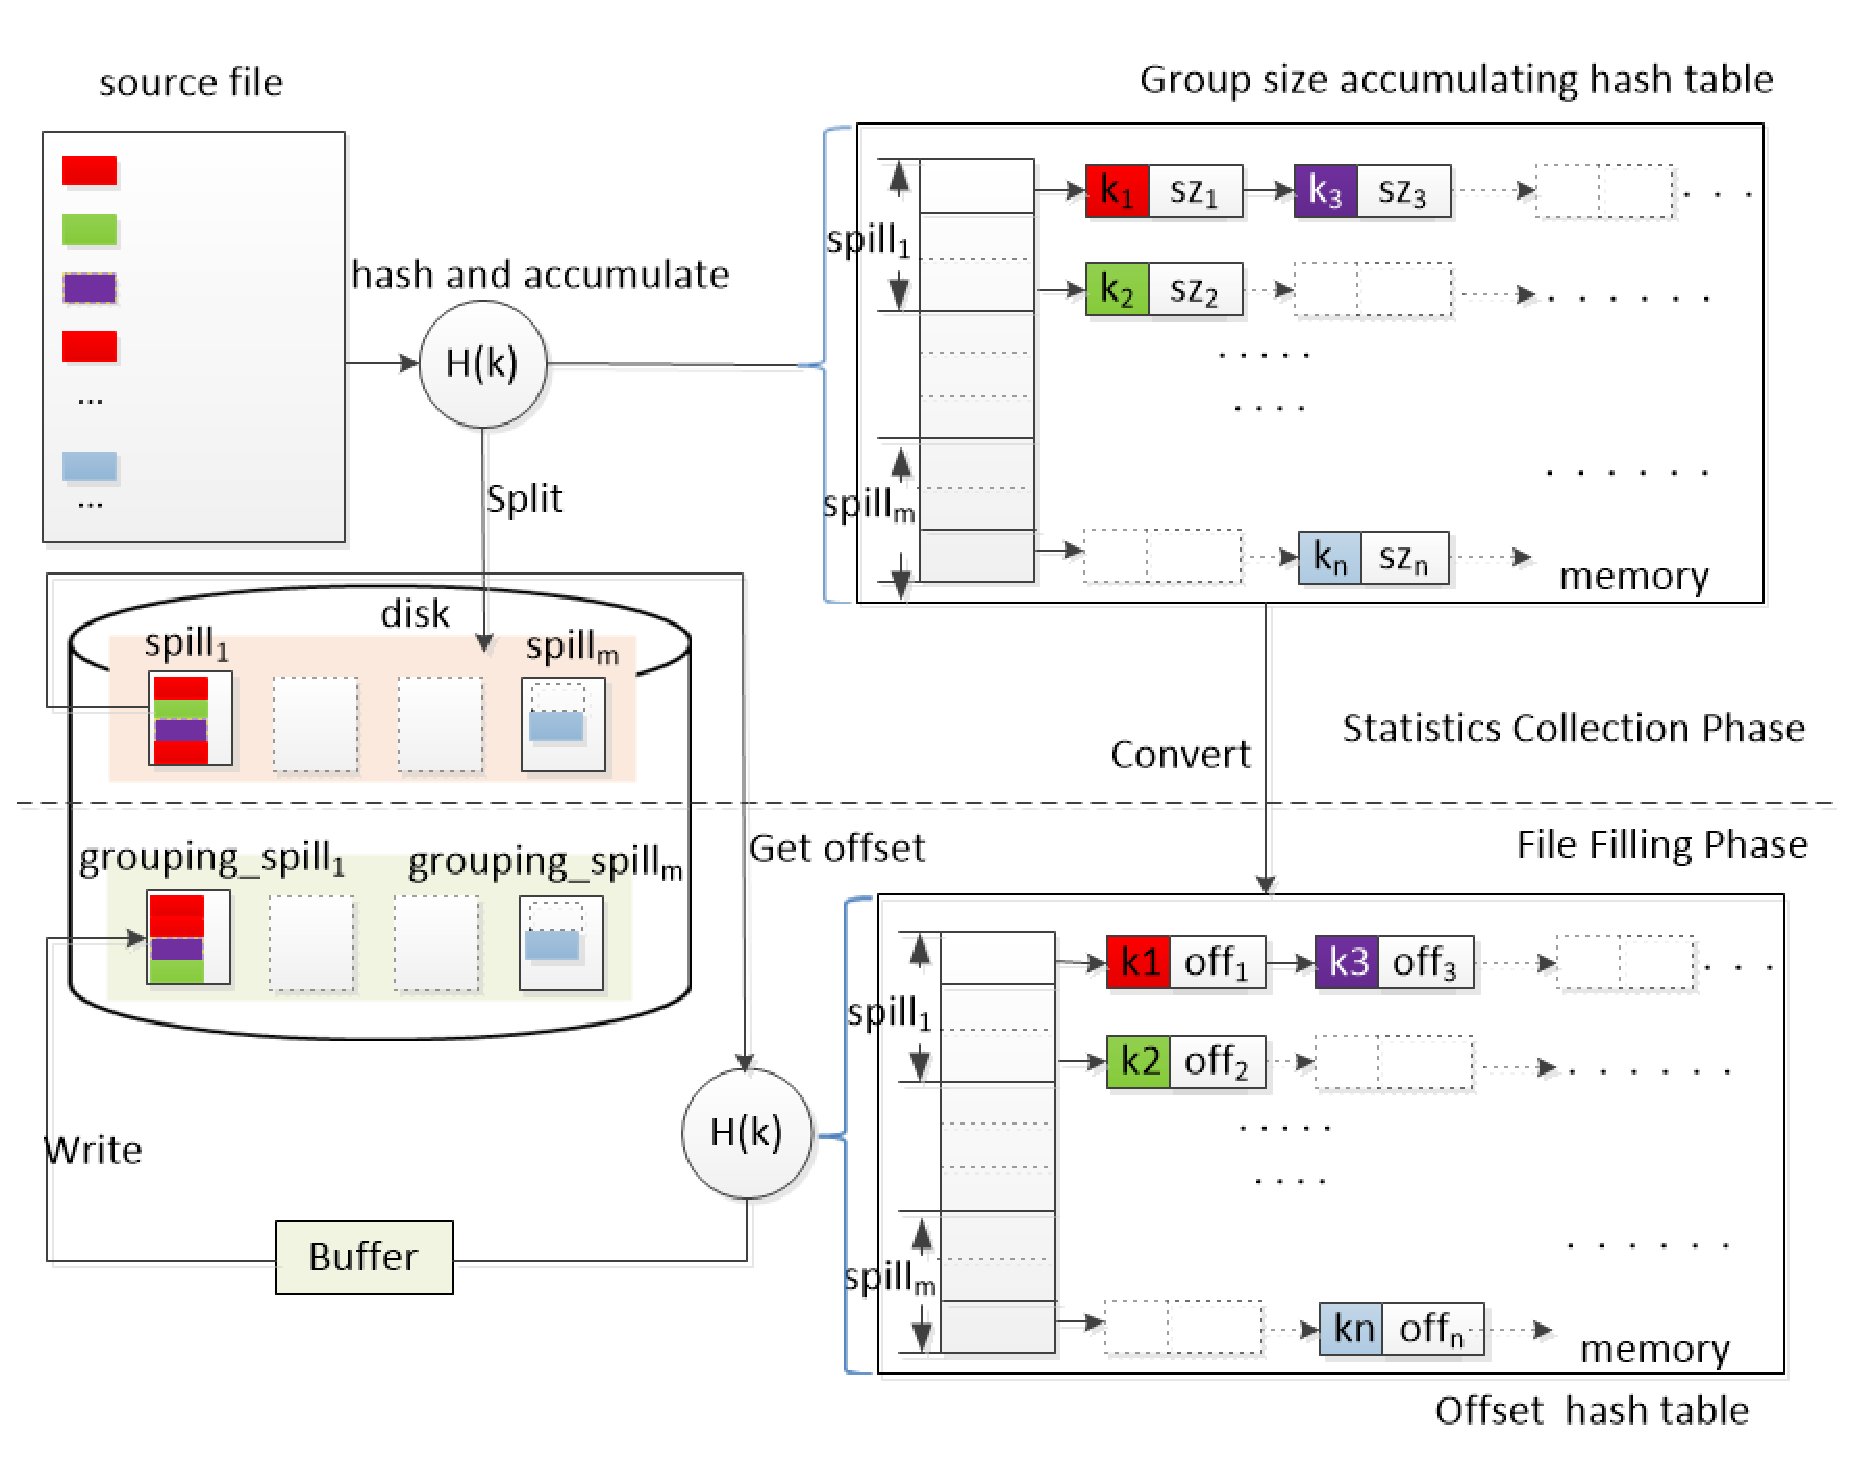
\includegraphics[width=.5\textwidth]{fig/bHash}
\caption{Overview Intuition of bHash.}
\label{fig:bHash}
\end{figure}

%\begin{figure}%figure 4
%\includegraphics[width=.5\textwidth]{Hashgroupingstage}
%\caption{Hash grouping phase.}
%\end{figure}

\subsection{Phase 1: Statistics Collection}%3.1

The first phase needs one pass of the whole input kv-pairs file and writes them out to multiple smaller files, which is referred to as \emph{spills}. In the first phase, multiple functions involved are described as follows.

%\Paragraph{Group Size Accumulation}

\textbf{Group Size Accumulation.} As shown in Figure \ref{fig:bHash}, an in-memory hash table is maintained to accumulate the value size for each key. The size of values indexed by the same key is accumulated in the value size table. By one pass of the whole set of input kv-pairs contained in source file we will obtain the value size table indexed by keys. Note that, the number of hash buckets $b$ in the group size table balances the memory cost and the query time cost, which will be discussed in Section \ref{sec:param}.


%\Paragraph{Kv-Pairs Reorganization}

\textbf{KV-Pairs Reorganization.} Recall that there is an output buffer (in the file filling phase) which aims at merging a large number of small random writes to less number of big sequential writes. If the random output kv-pairs are more concentrate on a key range, they are more likely to be continuously written out. That is, they can be merged together as less number of big sequential write. To improve the output buffer efficiency in the file filling phase, we should reorganize the read-in kv-pairs in a smart way.

Our idea is to partition the kv-pairs and assign the kv-pairs that are in the same partition with close write-out positions, such that the partition-by-partition processing of kv-pairs in file filling phase is likely to result in big sequential writes. Specifically, we partition the kv-pairs into multiple \emph{partitions}. This can be achieved by hashing, i.e., multiple $\langle key, value group \rangle$s sharing the same $H_g(key)$ are grouped together, where $H_g()$ is a hash function. The keys in the same partition are assigned with close write-out positions. These kv-pairs in the same partition are written out in a \emph{spill} as shown in Figure \ref{fig:bHash}. Note that, the recorded write-out position is not for the spill but for the final output file (i.e., grouping\_spill in Figure 2) with grouped kv-pairs.

%\Paragraph{Offset\_Table Generation}
\textbf{Offset\_Table Generation.} We then convert the value-size table to offset\_table. Given the size of each key and the size of values for each key, we can calculate how many bytes a $\langle key, value group\rangle$ pair will take up in the final output file. With a specific output order, we can calculate the write-out position (i.e., offset) for each $\langle key, value group\rangle$. As mentioned above, the output order should be determined according to the partition information. The $\langle key, value group \rangle$s in a partition are written out in a continuous order, so that these keys are assigned with continuous write-out positions. This can be done by incrementally assigning write-out positions partition-by-partition and within each partition.

%Let \emph{F} be the source file to be aggregated and \emph{T} be the group size accumulating hash table that each entry corresponds to a group. The phase mainly completes sub file division and group size accumulating. Let \emph{S} be the set of final grouping files and the dimension of \emph{S} is initialized by the sub file number \emph{m} specified by users. At the beginning, a empty hash table \emph{T} will be created, the basic array��s size has been set to \emph{b}, i.e., the number of hash buckets in table \emph{T}. If the number of hash buckets \emph{b} is too small, kv pairs mapped into one bucket will become a few more. The time of finding an entry in a hash table is proportional to the length of the bucket the record mapped to. However, too many hash buckets will require more memory, so the number of buckets \emph{b} must be an appropriate value to balance time cost and memory cost. Related parameters setting are given in section 4.

%$p_1^{t_1}$ $S=\{{p^{t_i}_i}\}^N_{i=1}$}

%It means that the hash table is partitioned horizontally into \emph{m} parts from top to down. The kv pairs mapped to the first $b/m$ buckets will be stored in sub file $file_0$ and mapped to the last $b/m$ buckets will be stored in sub file $file_{m-1}$ . After all the data in the source file has been processed, we can obtain the size of each group and kv pairs in the source file have been partitioned into several sub files. Each sub file represents an independent unit and groups among different sub files have no intersection, the key range covered by a sub file will be reduced by several multiples, which reduces the number of seek in the subsequent hash grouping phase.

\subsection{Phase 2: File Filling}%3.2

The offset\_table stores the output file position (i.e., offset) for each $\langle key, value group \rangle$. Given this deterministic information, the second phase runs as a file filling process by taking the spills as input. It reads in and processes the spills one by one. Referring to the in-memory offset\_table, the kv-pairs in spills are written out to specific positions in the final output file.

The profiling of this process shows that large amount of time is spent on seek operations during the file filling. This is mainly due to the fact that the writing of kv-pairs is not necessarily sequential. Recall that in the first phase the kv-pairs has been split into multiple partitions (i.e., spills) and their write-out positions have been reorganized from partition to partition. By processing each partition (spill) at a time, we can narrow the range of seek operations so as to reduce the seek distance (seek time).

%\Paragraph{Reordering KV-Pairs in Output Buffer}

\textbf{Reordering KV-Pairs in Output Buffer.} We have an output buffer design as shown in Fig 2. which buffers the write-out kv-pairs and reorders them according to their positions (i.e., offsets) before writing them out. It will 1) merge a large number of random small writes to less number of sequential big writes and 2) avoid frequent backward-and-forward disk arm movement. The ideal buffer size is equal to the size of an input spill, so that the buffer can hold all the kv-pairs in that spill. By using any $O(1)$ space requirement sorting algorithm (e.g., quick sort), we can sort these kv-pairs in terms of their offsets and output them with only one single sequential write without any random write operations.


%Without any extra reordering, we buffer these kv-pairs in their group entry of the offset table. Flushing the buffer only requires to traverse partial hash buckets that belong to the spill sequentially.
The spill size somehow depends on how the hash partition in the first phase is defined. We can set the hash partition function to generate more or less partitions to obtain smaller or bigger spills. However, the sizes of spills might be greatly different from each other due to the skewed data distribution. We cannot build a fix-sized buffer by assuming equal-sized spills. It is also possible that the memory budget is not enough to create the buffer when a certain spill is extremely large. A simple design is to buffer as many kv-pairs as possible and dump them together. Without any extra sorting, we buffer these kv-pairs in their group entries of the offset table. Flushing the buffer only requires to traverse partial hash buckets that belong to the spill sequentially. Because the offset of each group is calculated based on the previous entry, the offset for each group saved in hash entry is incremented sequentially bucket-by-bucket and within each bucket. In this way, seek operations of different groups will be in order, it allows us to flush the buffer by scanning sequentially the output file (i.e.,grouping\_spill). Note that, even though a random seek is performed, the seek time is expected to be very small because the next offset is physically very close to the current disk head position. The experiment shows that the gain is up to 10\%.
% Alternatively, we can borrow the idea from online live streaming which has a receive buffer for reordering the video packets \cite{}. It renders the video frames immediately as long as necessary packets have been received and at the same time releases the buffer space for future incoming packets. In our case, we have the similar requirements for the buffer design and can utilize XXX technique \cite{} to improve the buffer efficiency.

%\Paragraph{I/O Benefit Analysis}
\textbf{I/O Benefit Analysis.} In the following, we formally analyze the benefit of our \emph{partition-and-buffer} design that includes the $\langle key, value group \rangle$s partitioning in the first phase and the reordering buffer in the second phase. As known, the amount of I/O is the same no matter with or without the partition-and-buffer design. We focus on analyzing the seek distance, which plays a key role to I/O performance. We pose the following theorem to demonstrate the gained I/O benefit.

\begin{theorem}\label{theo:iobenefit}
Suppose without partitioning in the first phase, i.e., only one spill is produced after the first phase, with a fixed buffer size, it is required an expected total seek distance $D$ to generate the kv-pairs grouped output file. If we utilize partitioning and have $m$ spills, with the same buffer size, the expected total seek distance is $\frac{D}{m^2}$.
\end{theorem}
\begin{proof}
(1) Without partitioning. By using the buffer that reorders the kv-pairs in terms of their offsets, we can guarantee that the file filling after each buffer dumping never goes backward and forward. Suppose a buffer reorders $k$ unique keys with their values, and the average seek distance for writing each kv-pair is $d$. The total expected seek distance after each buffer dumping is $k\cdot d=D_b$.

(2) With partitioning. Since partitioning narrows the scope of key range by $\frac{1}{m}$, the average seek distance for writing each kv-pair is $\frac{d}{m}$. Furthermore, by partitioning the number of unique keys in buffer is also reduced to $\frac{k}{m}$ on average. The total expected seek distance after each buffer dumping is $\frac{k\cdot d}{m^2}=\frac{D_b}{m^2}$.

Since the amount of data is the same, the number of buffer dumping is the same for the above two cases, i.e., $\sum{D_b}=D$. Therefore, if there is total $D$ seek distance without partitioning, we only need $\frac{D}{m^2}$ seek distance with partitioning.
\end{proof}
%\subsection{Parallel Execution}
%phase 1: multiple I/O threads for spilling on SSD.
%phase 2: multiple processing threads and I/O threads for reordering every spill
%
%\textcolor{red}{this part is necessary for the completeness and can add credit. whether to implement it or not is up to you.}
\begin{algorithm}[ht]
    \caption{bHash}
  \label{tab:group}
    \begin{algorithmic}[1]
\Require  File \emph{F} , sub file number \emph{m} , hash buckets number \emph{b}
    \Ensure set of result files $R$
     \State \emph group size accumulating hash table \emph{T:=} a basic array of size \emph{b}
       \State \emph{S:=}\{\textbf{for} each \emph{i} \textbf{do} generate a file $spill_i$, \emph{0 $\textless$ i $\le$m}\}
         \State \emph{R:=}\{\textbf{for} each \emph{i} \textbf{do} generate a file $grouping\_spill_i$, \emph{0 $\textless$ i $\le$ m}\}
     \For{ each input $\langle key,value\rangle$ in \emph{F}}
      \State calculate the hash value H(key) on key
     \State check for a matching row in the hash table
     \If {there is no match}
     \State insert a entry (key,sizeof($\langle key,value\rangle$)) into \emph{T}
     \Else
     \State update the matching entry's group size with the sizeof($\langle key,value\rangle$)
     \EndIf
     \State $id=H(key)\%(b/m)$
     \State append the $\langle key,value\rangle$ to the partition file  $spill_{id}$
     \EndFor
     \State offset hash table $O:=Convert(T)$
     \For{ each $spill_i \in S$ ,\emph{0 $\textless$ i $\le$ m}}
     \For{ each input $\langle key,value\rangle$ in $spill_i$}
      \State calculate the hash value \emph{H(key)} on key
      \State $id=H(key)\%(b/m)$
     \State check for a matching key and get the $off_{key}$ of key from $O$
     \State write the $\langle key,value\rangle$ to the $off^{th}_{key}$ bytes of the file $grouping\_spill_i$
      \State the matching entry's offset is increased by sizeof($\langle key,value\rangle$)
     \EndFor
     \State remove the $spill_i$ from $S$
     \EndFor
    \State output \emph{R}
    \end{algorithmic}
\end{algorithm}
\subsection{Making Them Together}

We summarize the whole process including the first phase and second phase in Algorithm 1. The algorithm starts by creating a working set containing \emph{m} sub files. Then the entire input file \emph{F} is scanned to calculate the size of each group in the working set. For a kv pair, calculate the hash value $H_{key}$ , then check whether there is a matching grouping entry in the hash table. If there is no a matching entry whose key is equal to the current key, insert a new entry that the first key is the current key and the second group size is the size of current kv-pair in bytes. If there is a matching group already, update the matching entry's group size like Formula 1.
\begin{equation}\label{eq:freshness}
    f_{key} += sizeof(key)+sizeof(value).
\end{equation}
\par{The next step is to output the current kv-pair to sub file, the id of corresponding file can be obtained from Formula 2.}
\begin{equation}\label{eq:freshness}
    id = H(key)\%(b/m).
\end{equation}
It means that the hash table is partitioned horizontally into \emph{m} parts from top to down. The kv-pairs mapped to the first $b/m$ buckets will be stored in sub file $spill_1$ and mapped to the last $b/m$ buckets will be stored in sub file $spill_m$ . After all the data in the source file have been processed, we can obtain the size of each group and kv-pairs in the source file have been partitioned into several sub files(as shown 4-14 in algorithm 1).

Before the file filling phase really begins, we need to convert every group size to the file position information (i.e.,offset, see line 15 in Algorithm 1). The $Convert$ function traverses the group size accumulating hash table $T$, in more details, traverses hash buckets in the same partition from top to down and from left to right for a bucket. The first entry of the first bucket in the $i^{th}$ partition is the first group of the $i^{th}$ partition, so the initial offset of the entry equals to 0. The initial offset of an entry means that the first kv-pair mapped to the group will be stored in the ${(initial \; offset)}^{th}$ bytes of the grouping sub file $grouping\_spill_i$. Define the group size of the previous entry as $f_{pre}$, which means that the size of the previous group is $f_{pre}$. Define the initial offset of the previous group as ${off}_{pre}$. So the offset of current entry ${off}_{cur}$ equals to the sum of ${off}_{pre}$ and $f_{pre}$. After calculate the offset of each group, bHash will obtain an in-memory table which contains $\langle groupkey,fileposition\rangle$ information. Finally, File Filling phase needs another pass of the spilting file and outputs kv-pairs to file in terms of the previously obtained $\langle groupkey,fileposition\rangle$ information(see lines 16-25 in Algorithm 1). Each sub file $spill_i$ is a processing unit. The entire input split is scanned sequentially as shown in Figure 2. For a kv-pair, calculate the hash value $H_{key}$ and get the offset ${off}_{key}$  by searching the hash bucket $H_{key}$. Then, the kv-pair will be wrote to the ${off}^{th}_{key}$ bytes of the result file $grouping\_spill_{id}$. With a kv-pair from sub file $spill_{i}$ having been output, the current offset of the corresponding group will increase the size of the kv-pair in bytes, which indicates the next kv-pair mapped to the same group will be stored in the ${({off}_{cur} + sizeof(\langle key,value\rangle ))}^{th}$ bytes of the grouping sub file $spill_{id}$(line 22 in Algorithm 1). Specifically, some buffer optimizations have been applied as shown in section B. Grouping a sub file at a time, the key range is covered in a sub file, so the seek operation only appears in one file, which is the main reason of splitting.

To sum up, bHash benefits from both hash table��s random access ability (from hash-based grouping) and sorted structure��s sequential access ability (from sort-based grouping).

%\begin{algorithm}[ht]
%    \caption{Hash Grouping}
%  \label{tab:commands}
%    \begin{algorithmic}[1]
%\Require  set of sub files $S$, group size accumulating hash table $T$, sub file number $m$, hash buckets number $b$
%    \Ensure set of result files $R$
%     \State \emph{R:=}\{\textbf{for} each \emph{i} \textbf{do} generate a file $file_i$, \emph{0 $\le$ i $\textless$ m}\}
%       \State offset hash table $O:=Convert(T)$
%     \For{ each $file_i \in S$ ,\emph{0 $\le$ i $\textless$ m}}
%     \For{ each input $\langle key,value\rangle$ in $file_i$}
%      \State calculate the hash value H(key) on key
%      \State $id=H(key)\%(b/m)$
%     \State check for a matching key and get the $off_{key}$ of key from $O$
%     \State write the $\langle key,value\rangle$ to the $off^{th}_{key}$ bytes of the file $file_{id}$
%      \State the matching entry's offset is increased by sizeof($\langle key,value\rangle$)
%     \EndFor
%     \State remove the $file_i$ from $S$
%     \EndFor
%    \State output \emph{R}
%    \end{algorithmic}
%\end{algorithm}

\begin{comment}
The algorithm starts by creating a working set containing \emph{m} sub files (see Figure 3). Then the entire input file \emph{F} is scanned to calculate the size of each group in the working set. For a kv pair, calculate the hash value $H_{key}$ , then check whether there is a matching grouping entry in the hash table. If there is no a matching entry whose key is equal to the current key, insert a new entry that the first key is the current key and the second value size is the size of current kv pair in bytes. If there is a matching group already, update the matching entry's value size like Formula 1.
\begin{equation}\label{eq:freshness}
    f_{key} += sizeof(key)+sizeof(value).
\end{equation}
\par{The next step is to output the current kv pair to sub file, the id of corresponding file can be get from Formula 2.}
\begin{equation}\label{eq:freshness}
    id = H(key)\%(b/m).
\end{equation}


\begin{algorithm}[ht]
    \caption{Group Size Accumulating}
  \label{alg:group}
    \begin{algorithmic}[1]
\Require  File \emph{F} , sub file number \emph{m} , hash buckets number \emph{b}
    \Ensure set of sub files \emph{S}, group size accumulating hash table \emph{T}
     \State \emph{T:=} a basic array of size \emph{b}
       \State \emph{S:=}\{\textbf{for} each \emph{i} \textbf{do} generate a file $file_i$, \emph{0 $\le$ i $\textless$ m}\}
     \For{ each input $\langle key,value\rangle$ in \emph{F}}
      \State calculate the hash value H(key) on key
     \State check for a matching row in the hash table
     \If {there is no match}
     \State insert a new entry  [key,sizeof($\langle key,value\rangle$)] into \emph{T}
     \Else
     \State update the matching entry's value size with the sizeof($\langle key,value\rangle$)
     \EndIf
     \State $id=H(key)\%(b/m)$
     \State append the $\langle key,value\rangle$ to the partition file  $file_{id}$ in \emph{S}
     \EndFor
    \State output \emph{S}
    \end{algorithmic}
\end{algorithm}

It means that the hash table is partitioned horizontally into \emph{m} parts from top to down. The kv pairs mapped to the first $b/m$ buckets will be stored in sub file $file_0$ and mapped to the last $b/m$ buckets will be stored in sub file $file_{m-1}$ . After all the data in the source file has been processed, we can obtain the size of each group and kv pairs in the source file have been partitioned into several sub files. Each sub file represents an independent unit and groups among different sub files have no intersection, the key range covered by a sub file will be reduced by several multiples, which reduces the number of seek in the subsequent hash grouping phase.

During this phase, bHash constructs the grouping sub file for each sub file $file_i$. In Group Size Accumulating phase, the size of all groups has been accumulated in hash table. Before the hash grouping phase really begins, we need to convert every group size to the file position information (offset) of the group (line 2 in Algorithm 2). The $Convert$ function traverses the group size accumulating hash table $T$, in more details, traverses hash buckets in the same partition from top to down and from left to right for a bucket. The first entry of the first bucket in the $i^{th}$ partition is the first group of the $i^{th}$ partition, so the initial offset of the entry equals to 0. The initial offset of an entry means that the first kv-pair mapped to the group will be stored in the ${(initial \; offset)}^{th}$ bytes of the grouping sub file $file_i$. Define the group size of the previous entry as $f_{pre}$, which means that the size of data contained by the previous group is $f_{pre}$. Define the initial offset of the previous group as ${off}_{pre}$. So the offset of current entry ${off}_{cur}$ equals to the sum of ${off}_{pre}$ and $f_{pre}$. After calculate the offset of each group, bHash will obtain an in-memory table which contains $\langle groupkey,fileposition\rangle$ information. Finally, Hash Grouping phase needs another pass of the input file and outputs kv-pairs to file in terms of the previously obtained $\langle groupkey,fileposition\rangle$ information(see lines 3-12 in Algorithm 2). Each sub file $file_i$ is a processing unit. The entire input sub file is scanned sequentially as shown in Figure 4. For a kv-pair, calculate the hash value $H_{key}$ and get the offset ${off}_{key}$  by searching the hash bucket $H_{key}$. After getting the offset, the kv-pair will be wrote to the ${off}^{th}_{key}$ bytes of the result file $file_{id}$. With a kv-pair from sub file $file_{i}$ having been output, the current offset of the corresponding group will increase the size of the kv-pair in bytes, which indicates the next kv-pair mapped to the same group will be stored in the ${({off}_{cur} + sizeof(\langle key,value\rangle ))}^{th}$ bytes of the grouping sub file $file_{id}$(line 8 in Algorithm 2). Grouping a sub file at a time, the key range is covered in a sub file, so the seek operation only appears in one file, which is the main reason of splitting.


Contrary to previous key value grouping approaches, bHash provides us a method to build the grouping file without sorting. This is achieved using group size accumulating and hash grouping. In more detail, group size accumulating creates a group size hash table to record the size of different groups in bytes and splits the source file into several sub file in order to narrow the key range dealt with at a time. Then, Hash Grouping phase assumes the sorted file structure and computes every group's output position in the sorted file and do not really sort actually but only guarantee the kv-pairs in the same group to be locate together. To sum up, bHash benefits from both hash table��s random access ability (from hash-based grouping) and sorted structure��s sequential access ability (from sort-based grouping).
\begin{algorithm}[ht]
    \caption{Hash Grouping}
  \label{tab:commands}
    \begin{algorithmic}[1]
\Require  set of sub files $S$, group size accumulating hash table $T$, sub file number $m$, hash buckets number $b$
    \Ensure set of result files $R$
     \State \emph{R:=}\{\textbf{for} each \emph{i} \textbf{do} generate a file $file_i$, \emph{0 $\le$ i $\textless$ m}\}
       \State offset hash table $O:=Convert(T)$
     \For{ each $file_i \in S$ ,\emph{0 $\le$ i $\textless$ m}}
     \For{ each input $\langle key,value\rangle$ in $file_i$}
      \State calculate the hash value H(key) on key
      \State $id=H(key)\%(b/m)$
     \State check for a matching key and get the $off_{key}$ of key from $O$
     \State write the $\langle key,value\rangle$ to the $off^{th}_{key}$ bytes of the file $file_{id}$
      \State the matching entry's offset is increased by sizeof($\langle key,value\rangle$)
     \EndFor
     \State remove the $file_i$ from $S$
     \EndFor
    \State output \emph{R}
    \end{algorithmic}
\end{algorithm}


\subsection{Optimizing Disk Access}
The experimental evaluation and profiling of the Algorithm Hash Grouping shows that a significant amount of time is spent on seeking the result file. This is mainly due to the fact that the grouping process requires disk accesses that may not be sequential. Note that splitting has eliminated the seek operation among multiple files, which narrows the scope of disk head movement. As the Algorithm 2 shows that the algorithm groups a sub file at a time, we buffer partial grouping results in memory (see Figure 4) in order to write more kv-pairs per seek operation. If the buffer is full, these buffered partial grouping data will be flushed to the disk. Although partial grouping data of the same group has been buffered together and just need one seek operation, the seek operations of different groups may be out of order because kv-pairs from a sub file are out of order. To address this issue, we propose a novel buffer approach formed by modifying the entry structure of the group size accumulating hash table, as depicted in Figure 5.

\begin{figure}%figure 5
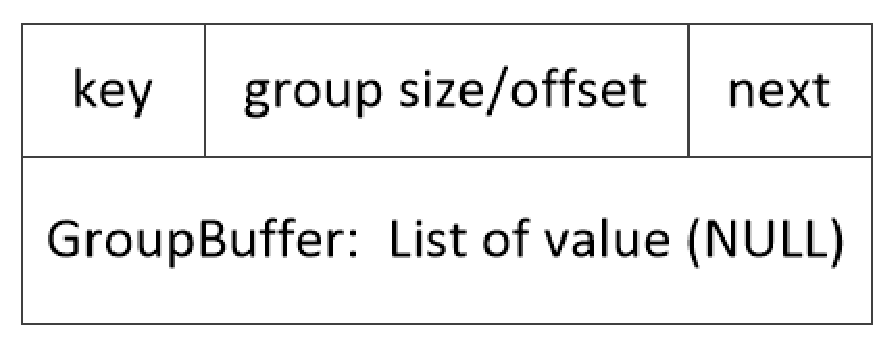
\includegraphics[width=.3\textwidth]{fig/EntryStructure}
\caption{the Entry Structure of the Group Size Accumulating Hash Table.}
\end{figure}
We buffer the partial grouping result in the entry of the hash table. During group size accumulating algorithm runs, the GroupBuffer filed is NULL in case of costing memory. With kv-pairs to be aggregated coming, values will be buffered in the entry that they belong to at first. The size of buffer used is the sum of the size of each GroupBuffer. If the size of buffer used achieves the maximum threshold, traverse the hash buckets contained by the sub file being processed and the partial grouping data will be output to the result file sequentially. Recall to 3.2 section, we convert the group size to the initial offset of a group. The offset of the current group ${off}_{cur}$ equals to the sum of ${off}_{pre}$ (the offset of the previous group) and  $f_{pre}$( the size of data contained by the previous group), which means that the stored location of the previous group must be prior to the current group. Thus, the seek operation for the current entry can base on the previous seek operation, i.e., the seek operations of all kv-pairs follow a top to down pattern in the result file. In this way, seek operations of different groups will be in order, it allows us to flush the buffer by scanning sequentially the result sub file. Note that, even though a random seek is performed, the seek time is expected to be very small because the next offset is physically very close to the current disk head position. The experiment shows that the gain is up to 10\%.
\end{comment}

%\subsection{Cost Analysis}

%Let $F$ be the input file, $n=|F|$ be the number of records, $G$ be the number of groups, $LB$ be the longest bucket in the hash table and $L$ be the largest linked list that stores the offset of each occurrence of a group for the bucket. In the worst case, $|LB|=O(n)$  and $|L|=O(n)$ . To see this, consider the input file $F$ for which $n=|F|$, each $\langle groupkey,valuesize\rangle$ are inserted to a hash bucket in group size accumulating phase, the worst complexity is $|L|$. The overall worst case complexity of group size accumulating is $n\cdot|L|$. For the hash grouping phase, each offset of a kv-pair needs to search the hash table, the query time is  $|L|$ in the worst case. The overall worst case complexity is also $n\cdot|L|$. Therefore, the overall worst case complexity of bHash is $2n \cdot|L|$ which is $O(n^2)$ time. However, in practice and in all application scenarios  $L \ll n$ and  $LB \ll n$ hold. The worst case above has supposed that is equal to $n$, e.g., each record is a group and all kv-pairs are mapped to a bucket. In fact, it is unusual because the target of the Hash technology is to uniform hash. The time to query and insert the hash table is almost constant order of magnitude so it is reasonable to expect that $L$ and $B$ are orders of magnitude far smaller than $n$. Thus, the overall expected complexity bound of bHash is much better than the worst case bound. This is also verified by the experimental evaluation, which demonstrated that bHash scales almost linearly to $n$.



\section{Discussions}
\label{sec:param}

\subsection{Key Parameters Analysis}

This overhead depends on certain bHash parameters: the hash bucket number, the sub file number, the sub-file buffer size and the grouping buffer size. A model for the optimal selection of these parameters is given in this section. We will expand our analysis from two aspects: disk access and memory consumption. For better analysis, we first define the following identifiers: the total data size $M$ (in bytes), the number of different groups $G$, the average size of each data $r$ (in bytes), thus, the total number of data is
\begin{equation}\label{eq:numberofdata}
  N=\frac{M}{r}
\end{equation}
the number of buckets $b$, the number of small source files $f$, the sub-file buffer size $e$, the size of grouping buffer $g$(in bytes).

\textbf{Disk Access}. the total number of reading disk is fixed, so we will focus on analysing the cost of writing disk. The first round of writing disk occurs when the source file is divided into some small partition files. The number of partition files is $f$, the total number of data records is $N$, then each partition file contains  $n=\frac{N}{f}$ records (assuming that the randomness of Hash makes data distributed uniformly). The number of a sub-file buffer being filled up by the data from a partition file is $\lceil\frac{n}{e}\rceil$ and a disk access will be generated for each flush buffer, then $f$ sub files will access disk $S_1$ times.
\begin{equation}\label{eq:numberofdata}
  S_1=f\cdot \lceil\frac{n}{e}\rceil=f\cdot\lceil\frac{N}{f\cdot e}\rceil \approx \frac{N}{e}=\frac{M}{e\cdot r}
\end{equation}
The second round of writing disk occurs in file filling phase. Recall to file filling phase, the data in each spill is retrieved and written to output file according to the offset in the hash table. The grouping buffer (as shown in Figure 2) can buffer $\frac{g}{r}$ kv-pairs before a flush operation is triggered. One flush may contains some disk seeks, but some disk access optimizations have been applied(recall reordering kv-pairs in section \uppercase\expandafter{\romannumeral3}) which can ensure the seek is sequential and the seek time is expected to be very small because the next offset is physically very close to the current disk head position. Thus, we simplify a flush as one disk access. The number of the grouping buffer being filled up by the data from a spill is $\lceil\frac{n}{g/r}\rceil=\lceil\frac{n\cdot r}{g}\rceil$, then the file filling phase need access disk $S_2$ times.
\begin{equation}\label{eq:numberofdata}
  S_2=f\cdot \lceil\frac{n\cdot r}{g}\rceil=f\cdot\lceil\frac{N\cdot r}{f\cdot g}\rceil \approx \frac{N\cdot r}{g}=\frac{M}{g}
\end{equation}
Therefore, the total number of accessing disk as shown in Formula 6.
\begin{equation}\label{eq:numberofdata}
  S=S_1+S_2=f\cdot\lceil\frac{N}{f\cdot e}\rceil + f\cdot\lceil\frac{N\cdot r}{f\cdot g}\rceil \approx \frac{M}{e\cdot r}+\frac{M}{g}
\end{equation}

\textbf{Memory Consumption}. Memory consumption is dominated by the hash table in memory and other two buffers. bHash uses sub-file buffer to
 store kv-pairs in statistics collection phase and grouping buffer to store grouping results data; therefore, sub-file buffer and grouping buffer can be safely overwritten. we use zipper method to implement the hash table. the memory consumption is consist of basic array and group size entries for each unique key. Suppose that the size of an element in basic array is $v_{array}$ and the size of entry is $v_{entry}$, then the total size of hash table $V_1$ is shown in Formula 7.
 \begin{equation}\label{eq:numberofdata}
  V_1=b\cdot v_{array}+ G\cdot v_{entry}
\end{equation}
Let's discuss the peak value of memory used in dividing the source file into sub files, it is obvious that the peak occurs when each sub-file buffer is full at the same time. Then the memory usage $V_2$ is $f\cdot e\cdot r$. In Hash Grouping phase, bHash just groups a sub file at a time, then the maximum memory usage during grouping process $V_3$ equals $g$. So the total memory usage is shown in Formula 8.
\begin{equation}\label{eq:numberofdata}
  V=V_1+ max(V_2,V_3)=b\cdot v_{array}+ G\cdot v_{entry}+ max(f\cdot e\cdot r,g)
\end{equation}
We group each sub file sequentially, it is best that the grouping buffer size is less than or equal to the amount of a sub file. A larger buffer will make kv-pairs buffered involve multiple sub files, which brings more unnecessary disk seek. In general, $V_2\textgreater V_3$, so Formula 8 can be simplified as formula 9.
\begin{equation}\label{eq:numberofdata}
  V=b\cdot v_{array}+ G\cdot v_{entry}+ f\cdot e\cdot r
\end{equation}

 If the maximum memory space $V$ is given, the relationship between memory usage and disk access can be deducted as follows by combining formula 6 and 9.
 \begin{equation}\label{eq:numberofdata}
  S=\frac{M\cdot f}{V-b\cdot v_{array}- G\cdot v_{entry}}+\frac{M}{g}
\end{equation}
When available memory size is fixed, the number of buckets $b$ increases or grouping buffer size $g$ decreases which both result the increase of disk I/O. At the same time, more different groups $G$, e.g., the data is more dispersed, a buffer may involve more groups, means that one flush will contain more seeks, therefore, the number of disk access $S$ will increase as shown in Formula 10. In fact, when $b$ reaches a certain threshold, the effect of the number of hash buckets on the time performance and memory usage is very little. In addition, it is easy to understand that larger buffer will reduce disk I/O cost and improve the Performance. The experimental evaluation for bHash parameters is shown in section \uppercase\expandafter{\romannumeral5}.

%\subsection{Use Cases}
%
%plug in, build plugin support for database groupby

\section{Experimental Evaluation}

\begin{figure*}%figure 6
    \centering
    \subfloat[Running time comparison with various data sets.]{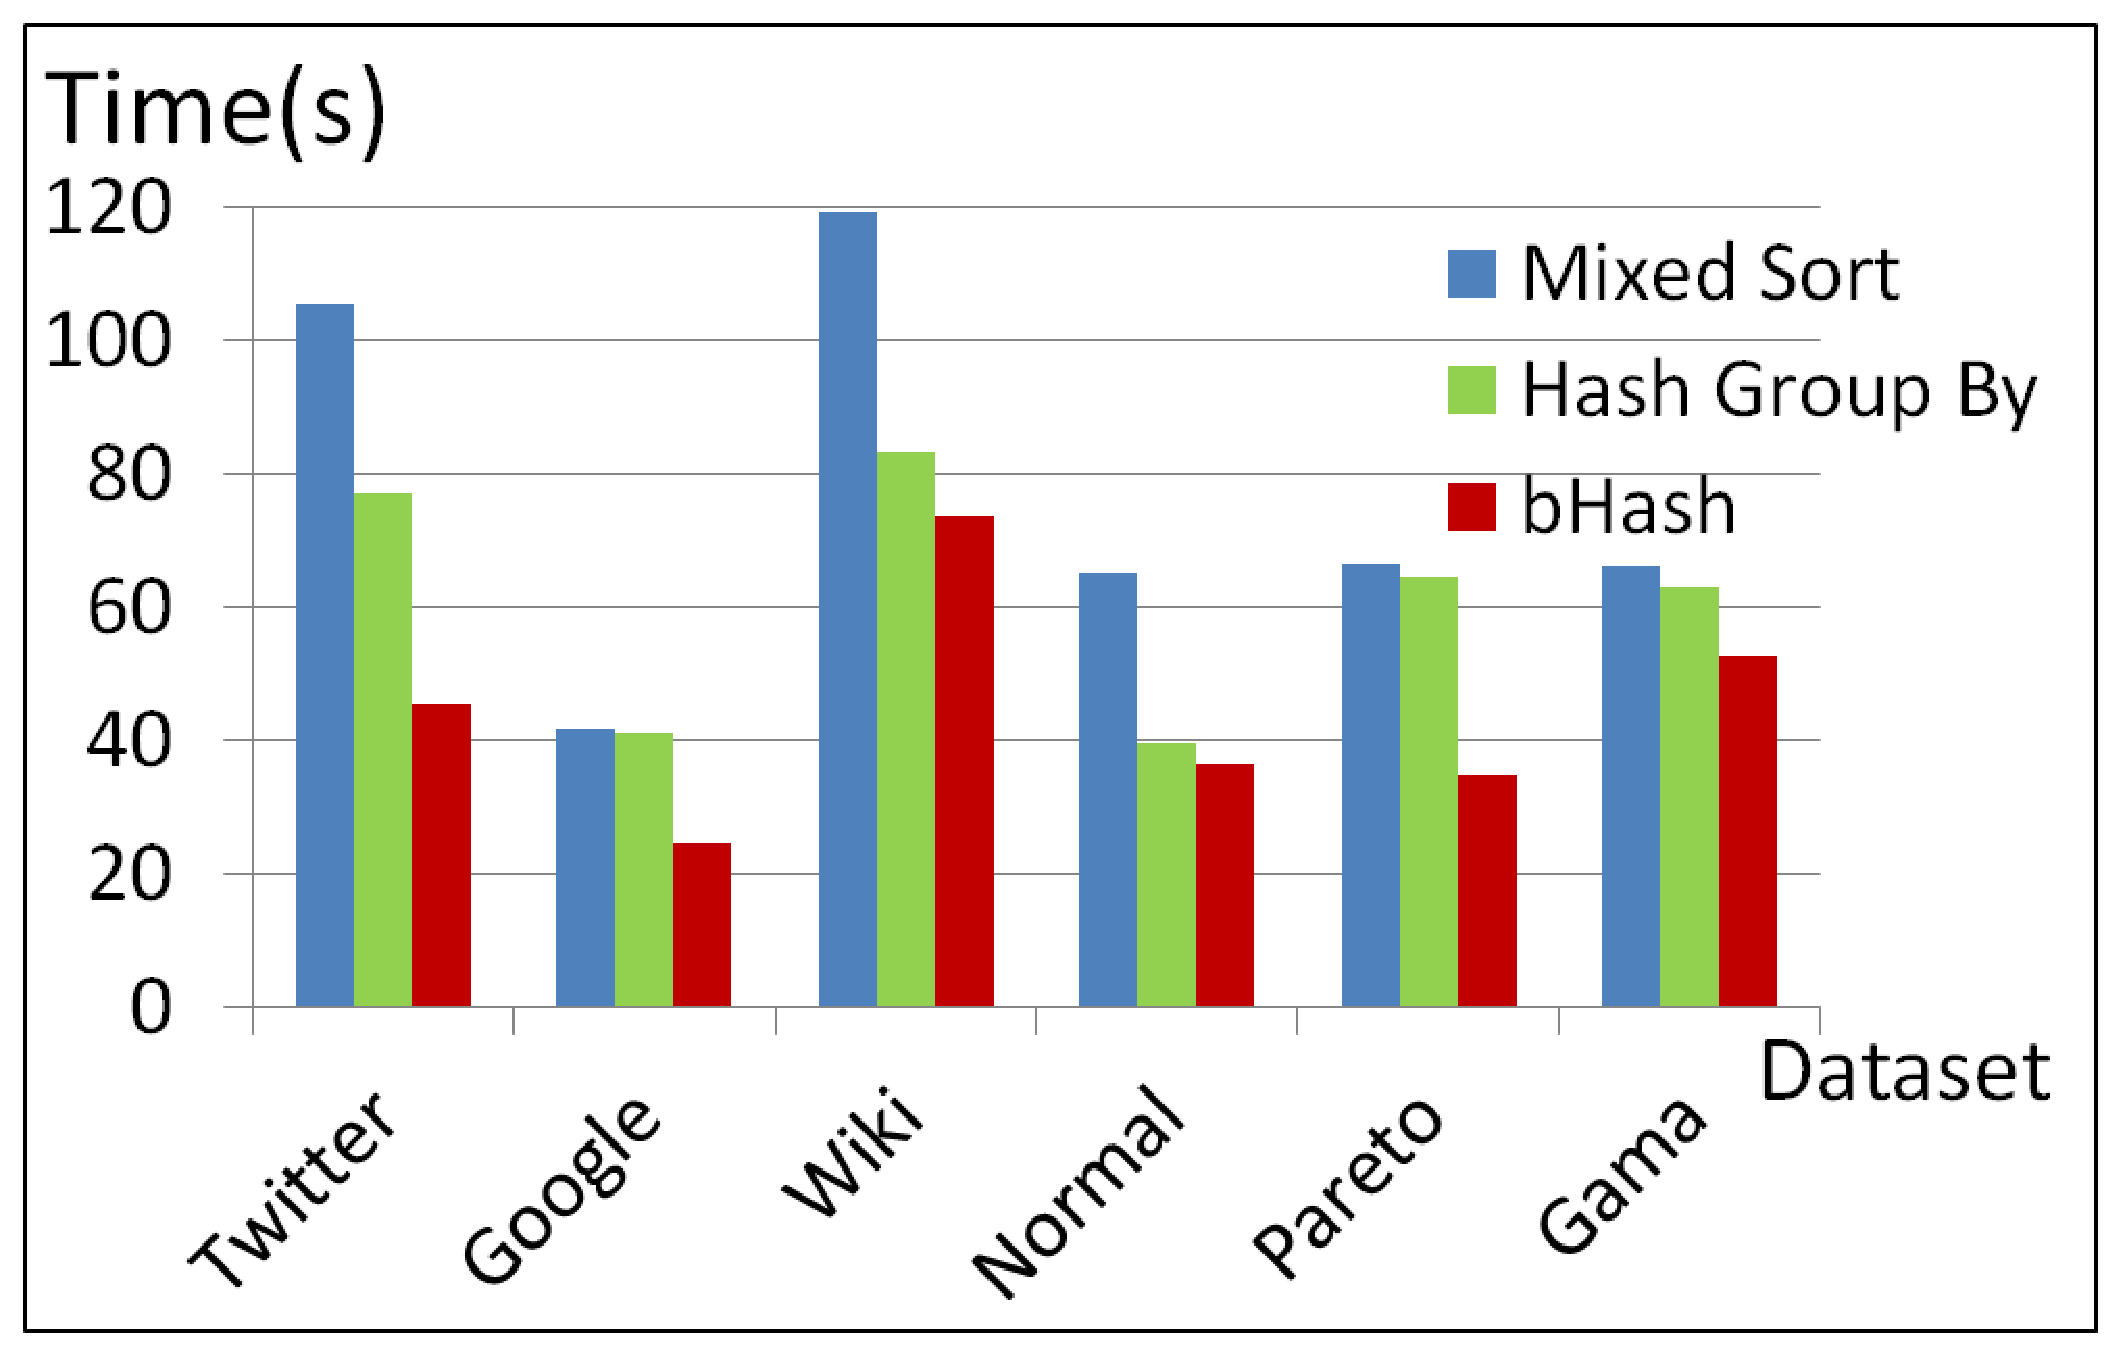
\includegraphics[width = 2in]{fig/datasetTime.eps}\label{fig:datasetTime}}\ \
    \hspace{1pt}
    \subfloat[Acceleration percentage compared with merge-sort]{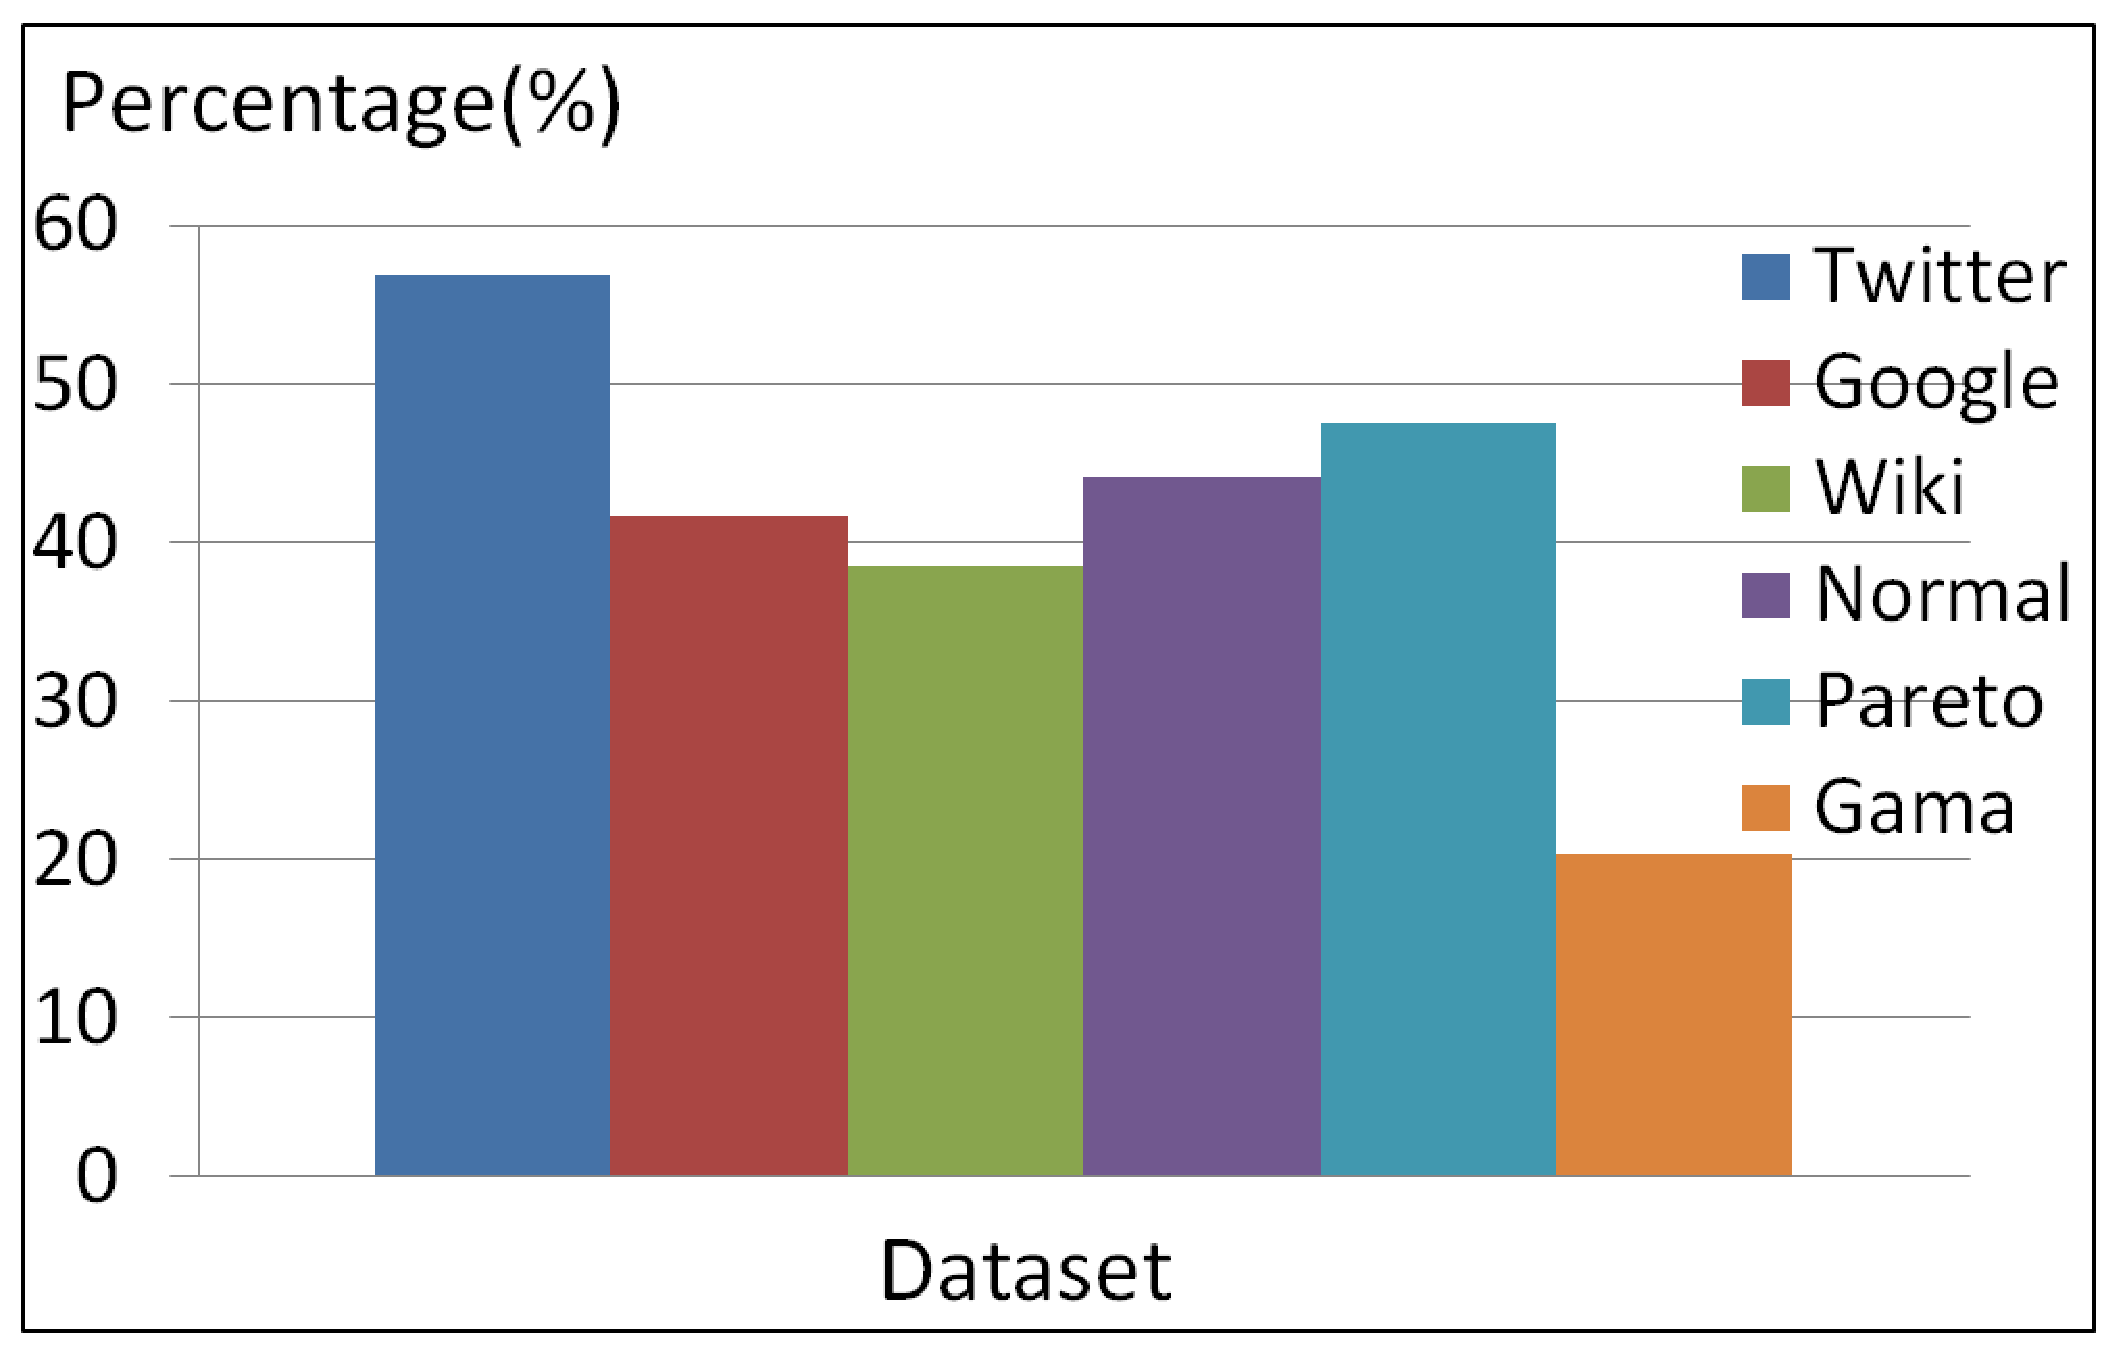
\includegraphics[width = 2in]{fig/percentageComparedSort.eps}\label{fig:percentageComparedSort}}\ \
    \hspace{1pt}
    \subfloat[Acceleration percentage compared with memory-constraint hash]{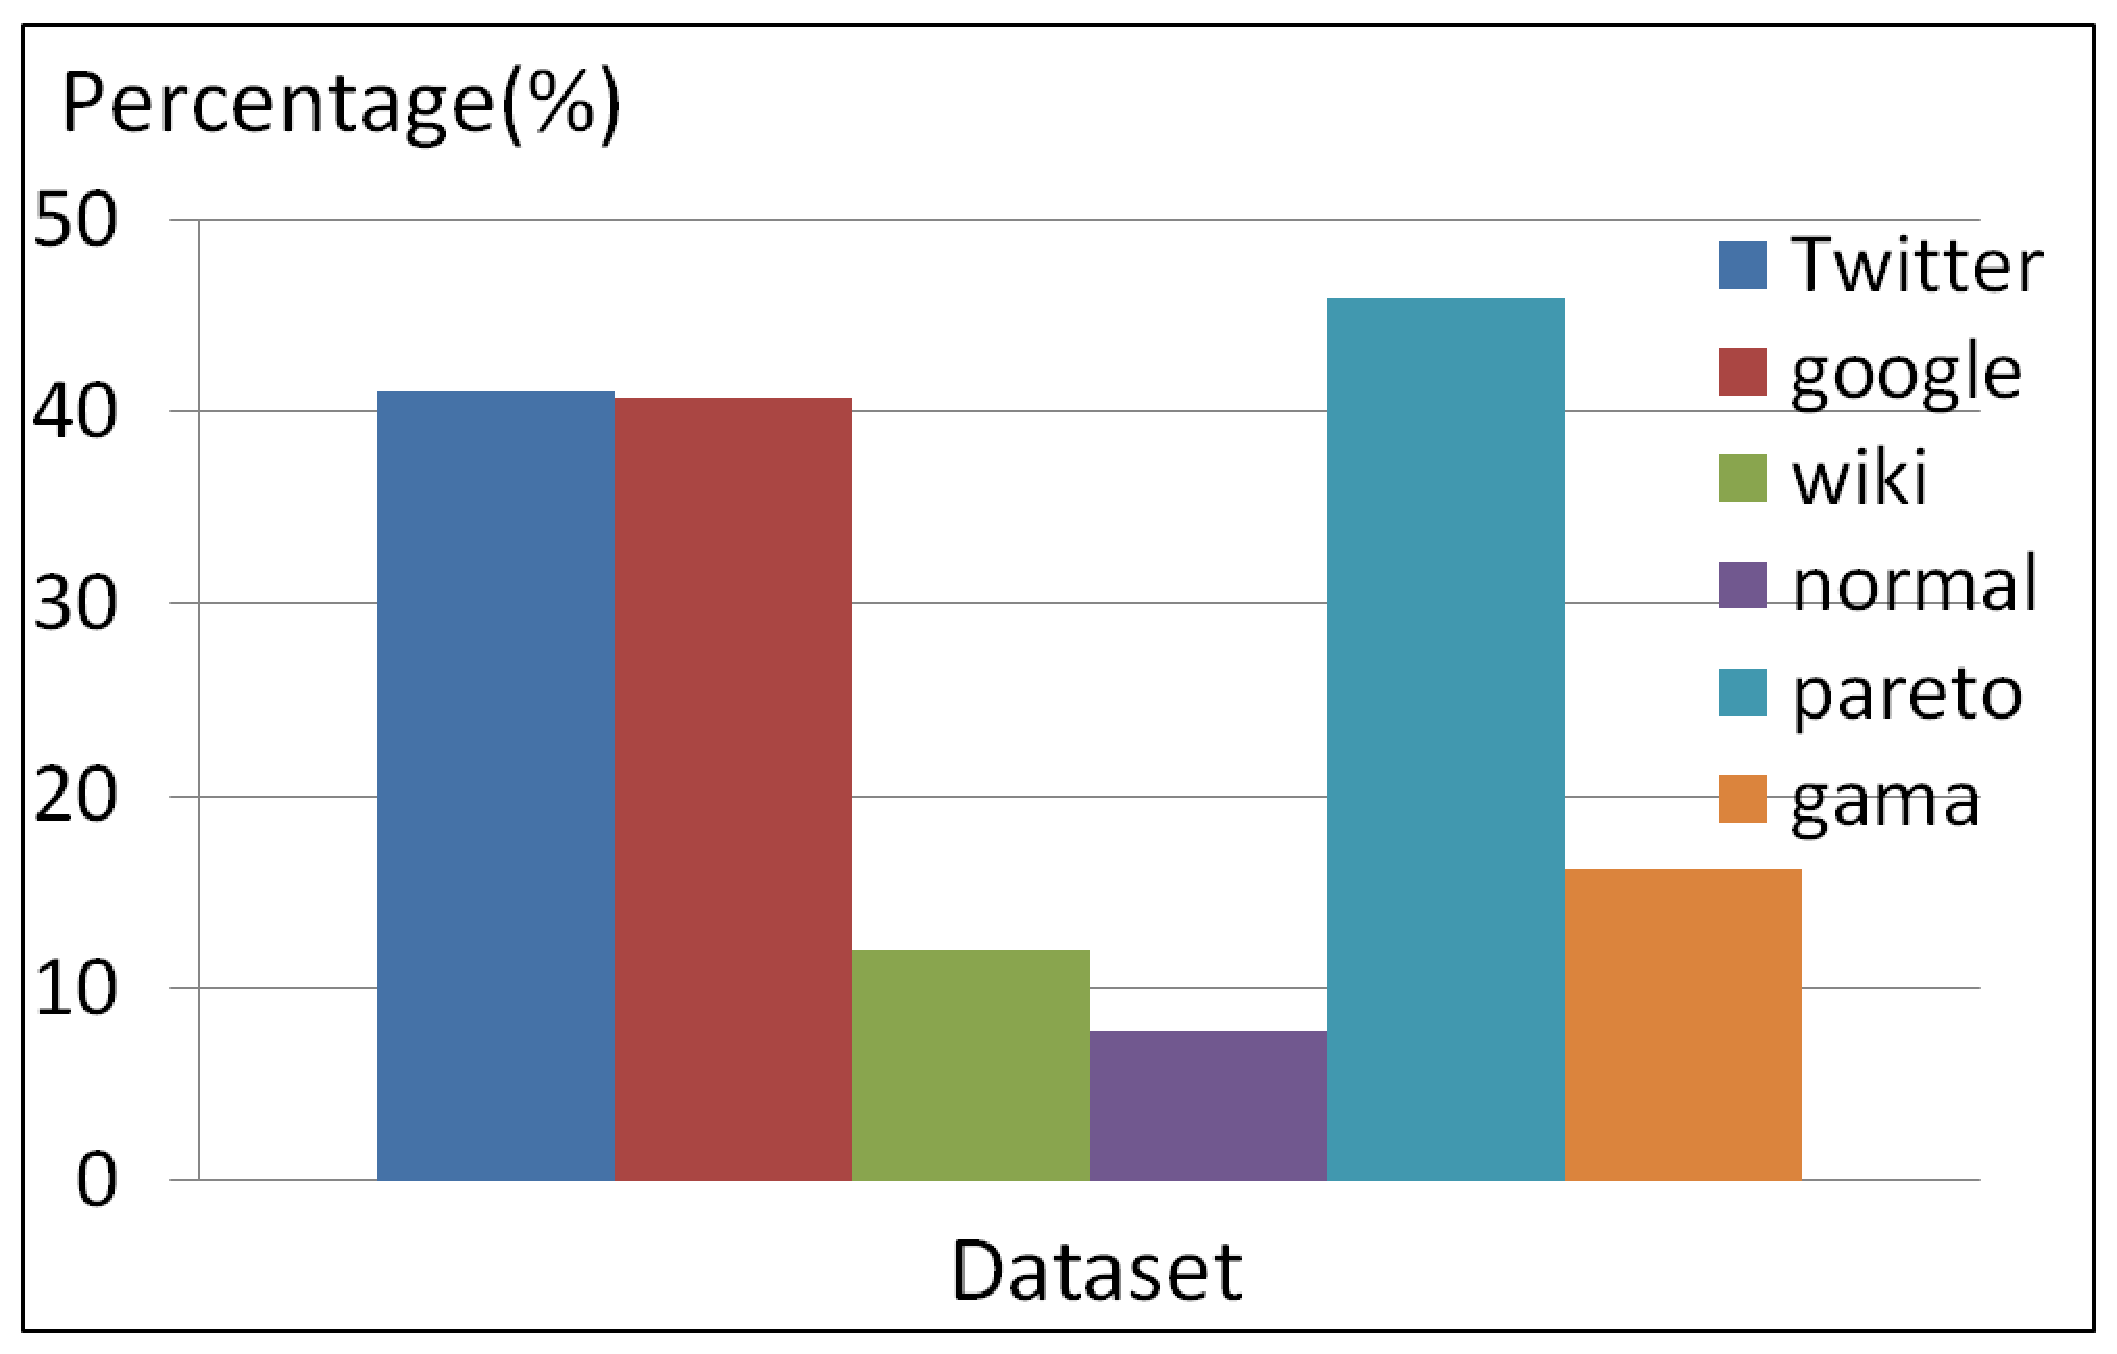
\includegraphics[width = 2in]{fig/percentageComparedHashGroupBy.eps}\label{fig:ComparedHashGroupBy}}\ \
    \caption{Running time and acceleration percentage under the same memory usage.}\label{fig:Running time and acceleration}
\end{figure*}

This section presents the performance evaluation for bHash. We compare our work against existing typical grouping approaches, merge-sort \cite{dean2008mapreduce} and memory-constraint hash \cite{bartholomew2012mariadb}. For merge-sort, we downloaded the implementation from the official sites. There is no source code for memory-constraint hash available, so we implemented our own hash aggregation version following the pseudo code in SQL database \cite{HashAggregate15}. We used typical real data sets:  (a) the Higgs\footnote{www.wikibench.eu/wiki/2007-09/wiki.1190153705.gz} Twitter data set, providing the information about activity on Twitter during the discovery of Higgs-boson; (b) the Google\footnote{http://snap.standford.edu/data/web-Google.txt.gz} web graph data set containing 870,000 nodes and 5,100,000 edges; (c) the Wiki\footnote{http://snap.standford.edu/data/higgs-twitter.html} data set containing 1.2GB different URLs; and three simulation data sets that obey different distributions including a Normal distribution and two weight-tailed distributions : Pareto and Gama. Table 1 summarizes the data sets used.

\begin{figure*}
    \centering
    \subfloat[Performance comparison on Wiki]{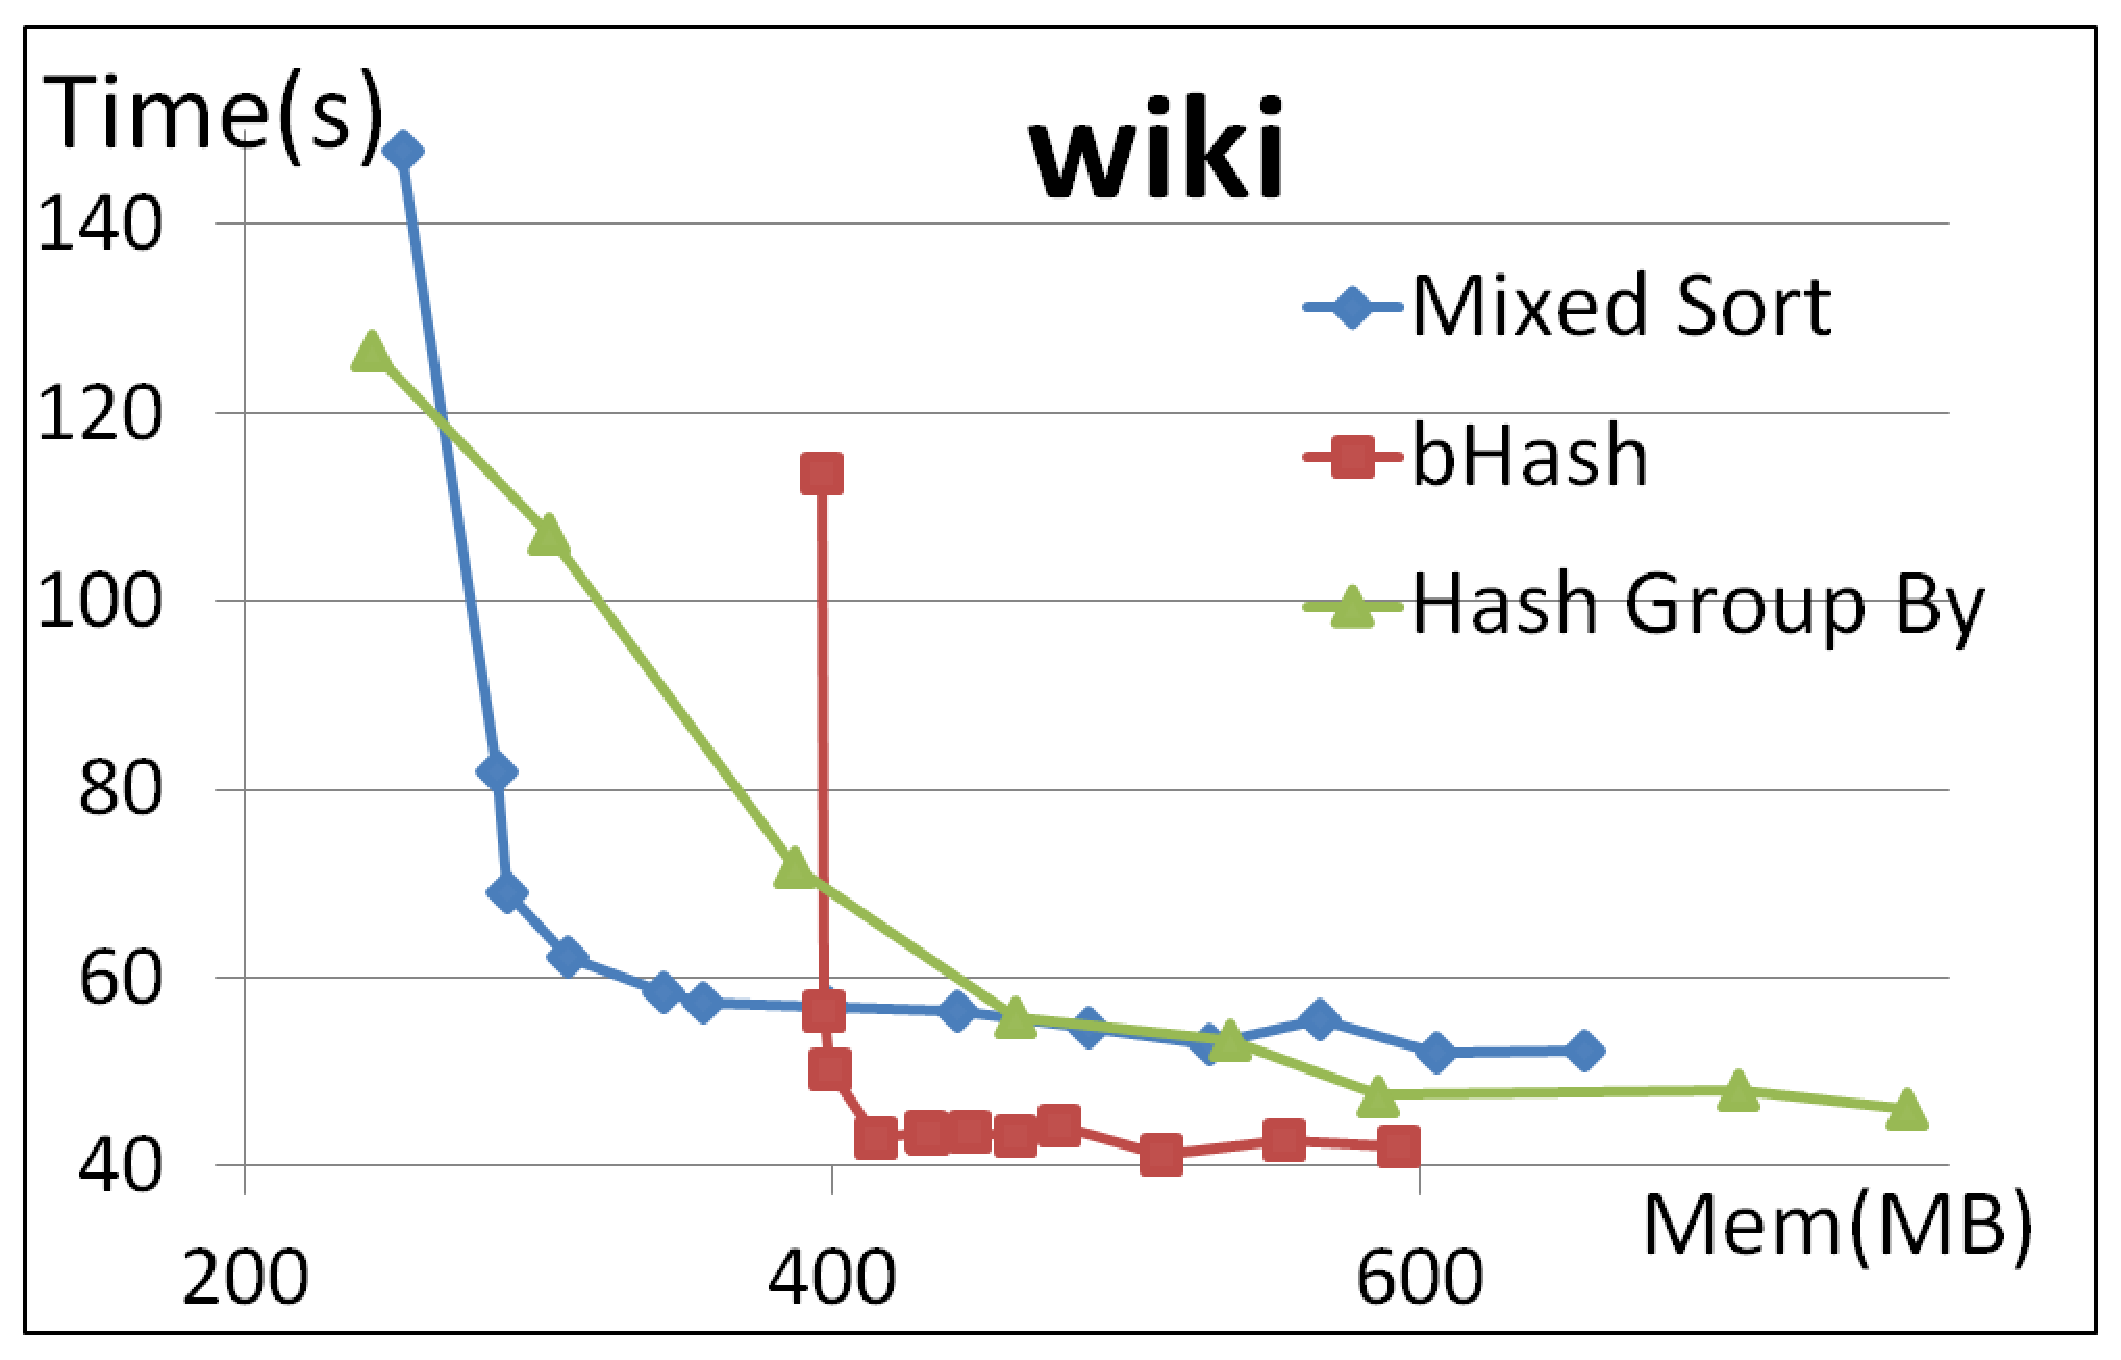
\includegraphics[width = 1.61in]{fig/wikiMemTime.eps}\label{fig:wikiMemTime}}\ \
    \hspace{0.5pt}
    \subfloat[Performance comparison on Twitter]{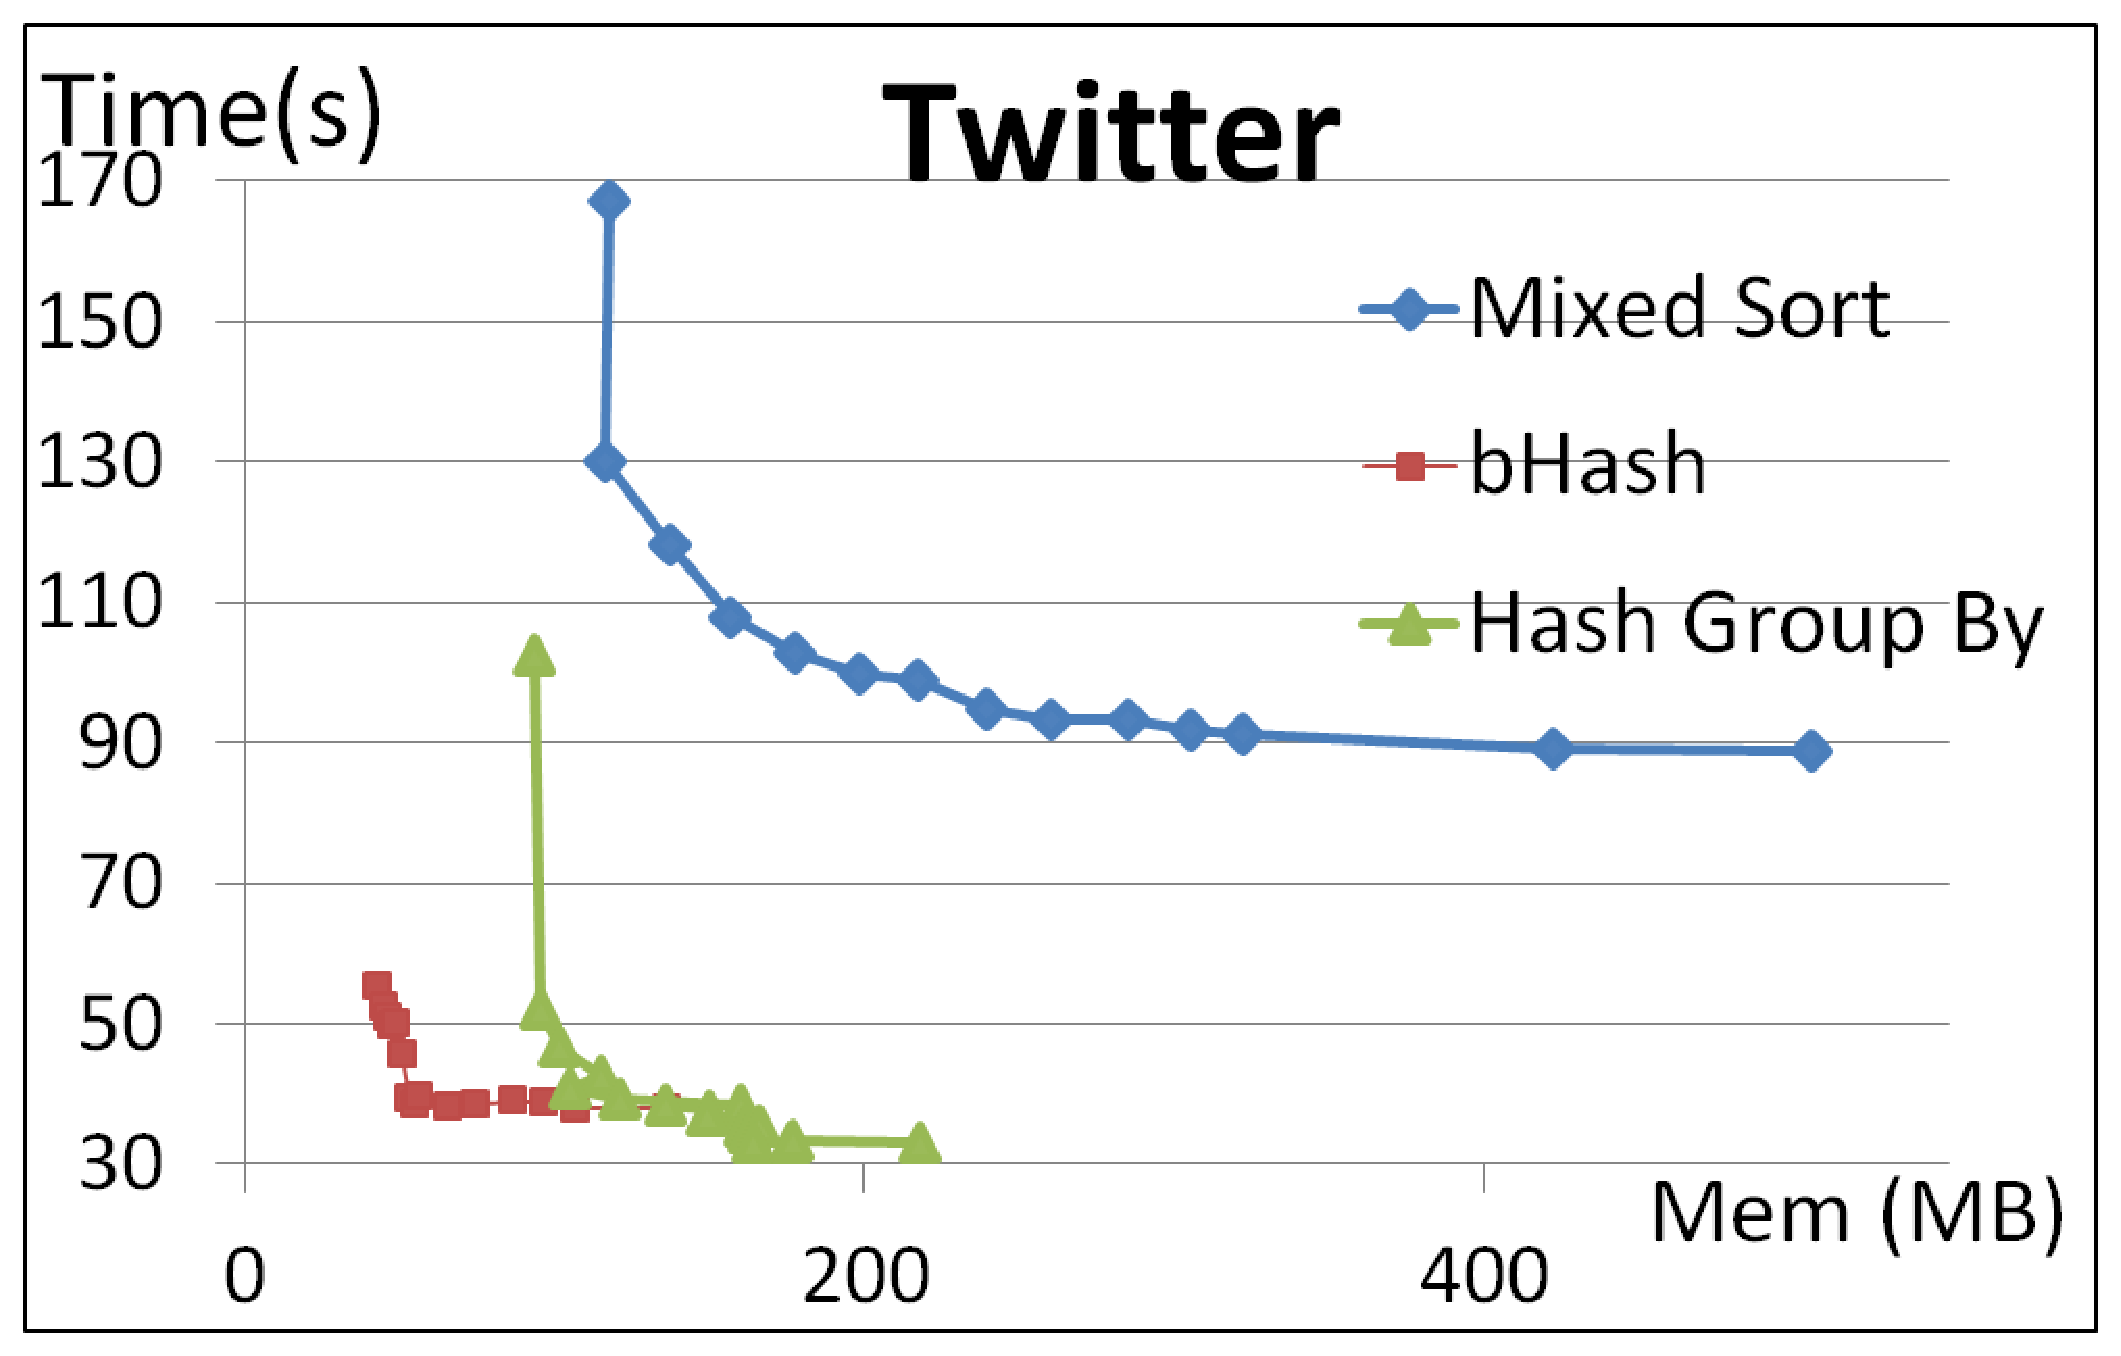
\includegraphics[width = 1.61in]{fig/twitterMemTime.eps}\label{fig:twitterMemTime}}\ \
   \hspace{0.5pt}
    \subfloat[Performance comparison on Normal]{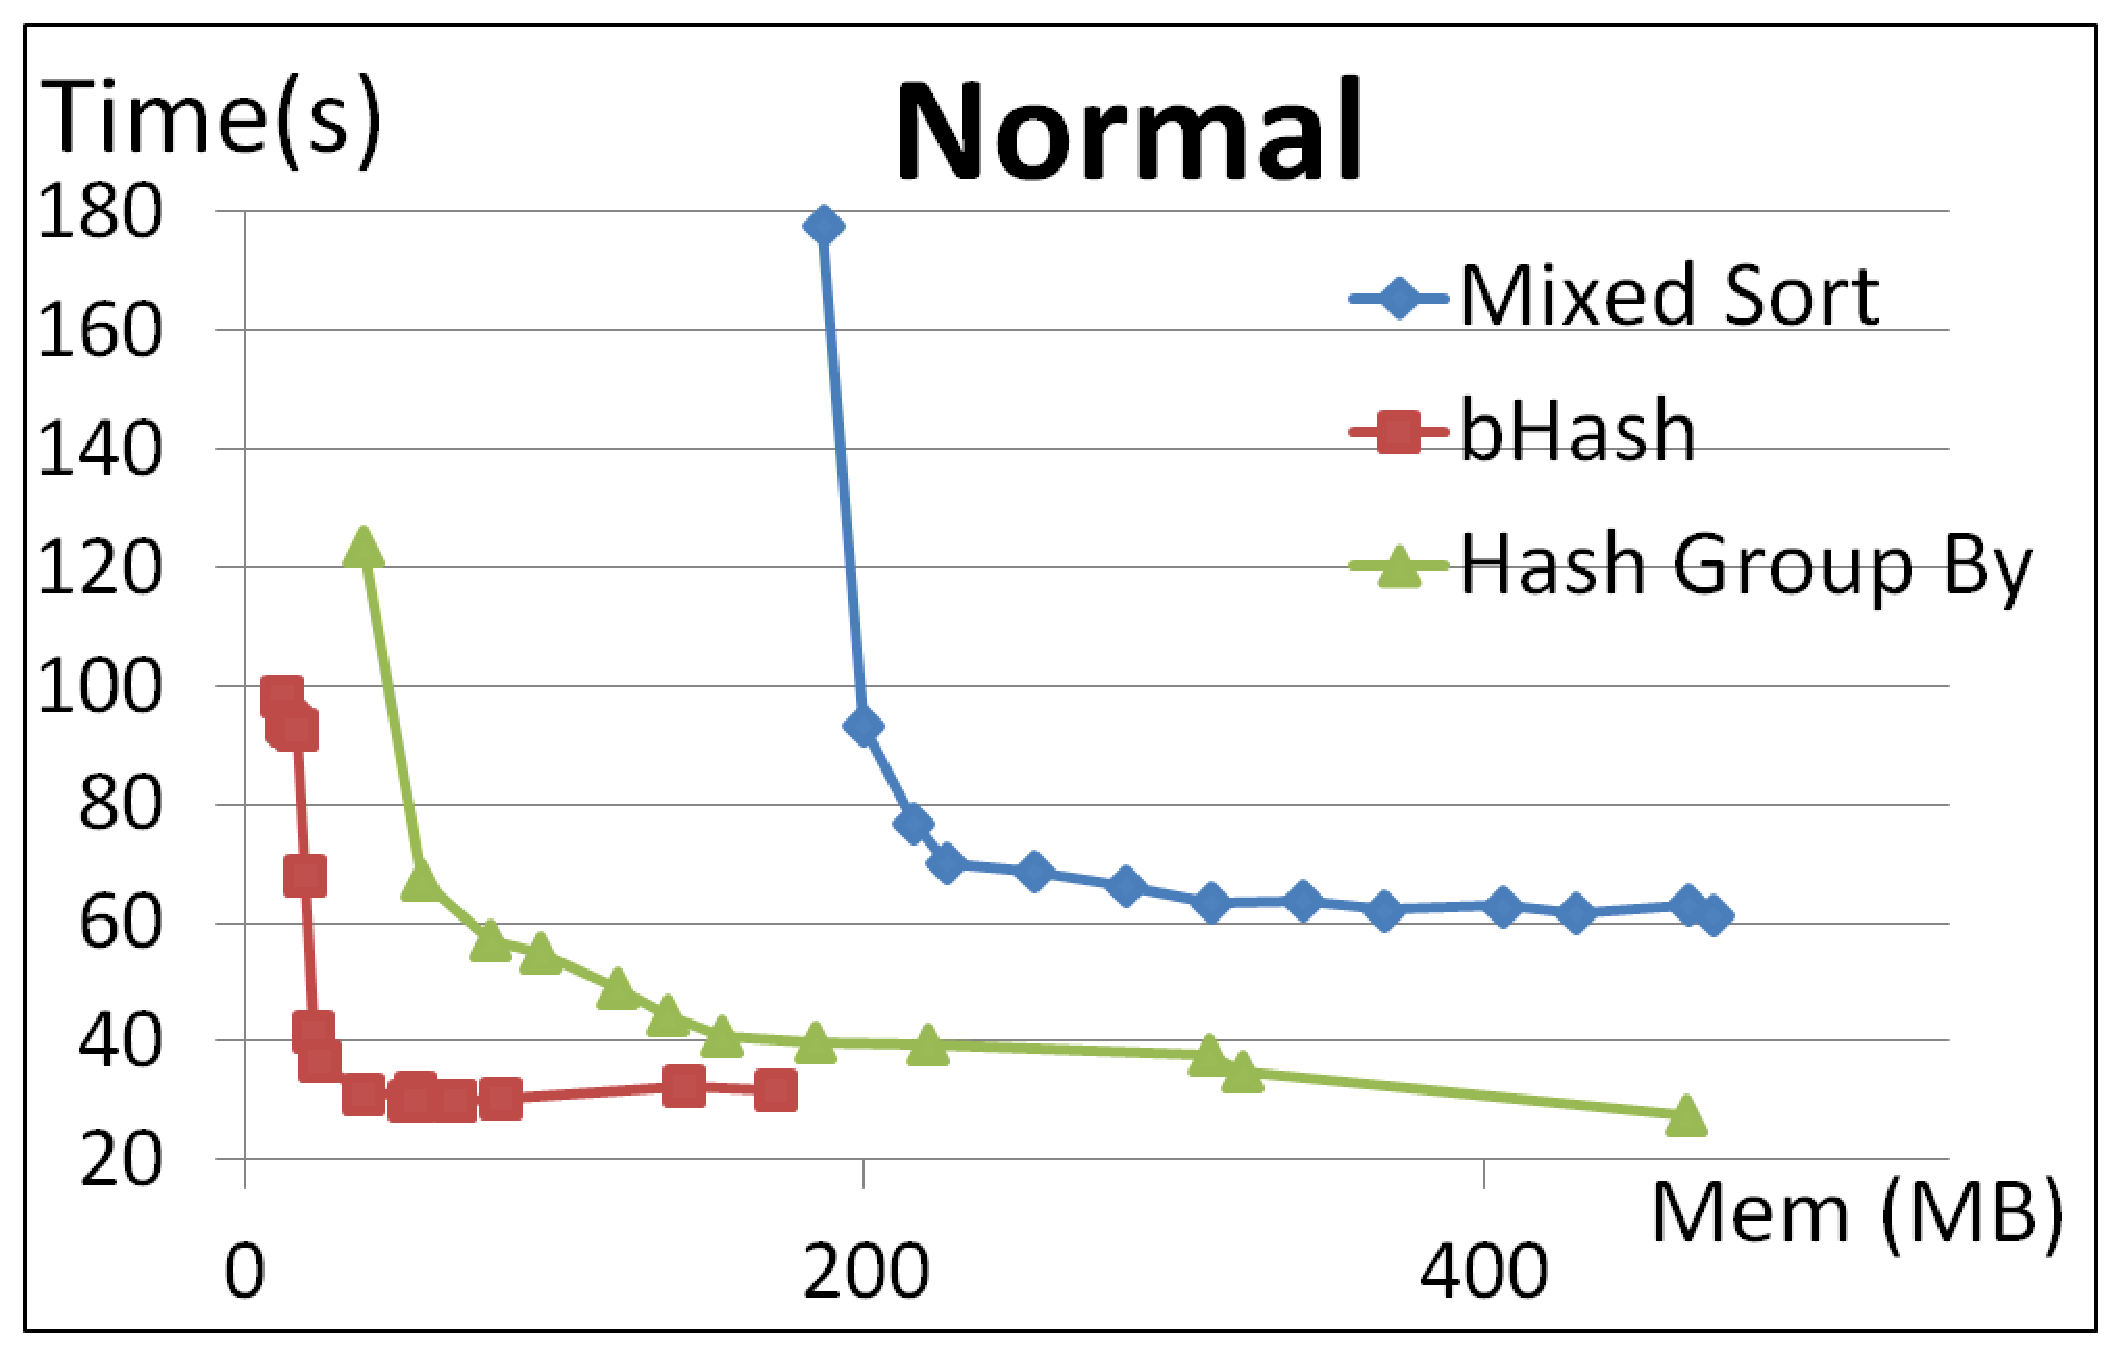
\includegraphics[width = 1.61in]{fig/normalMemTime.eps}\label{fig:normalMemTime}}\ \
     \hspace{0.5pt}
    \subfloat[Performance comparison on Pareto]{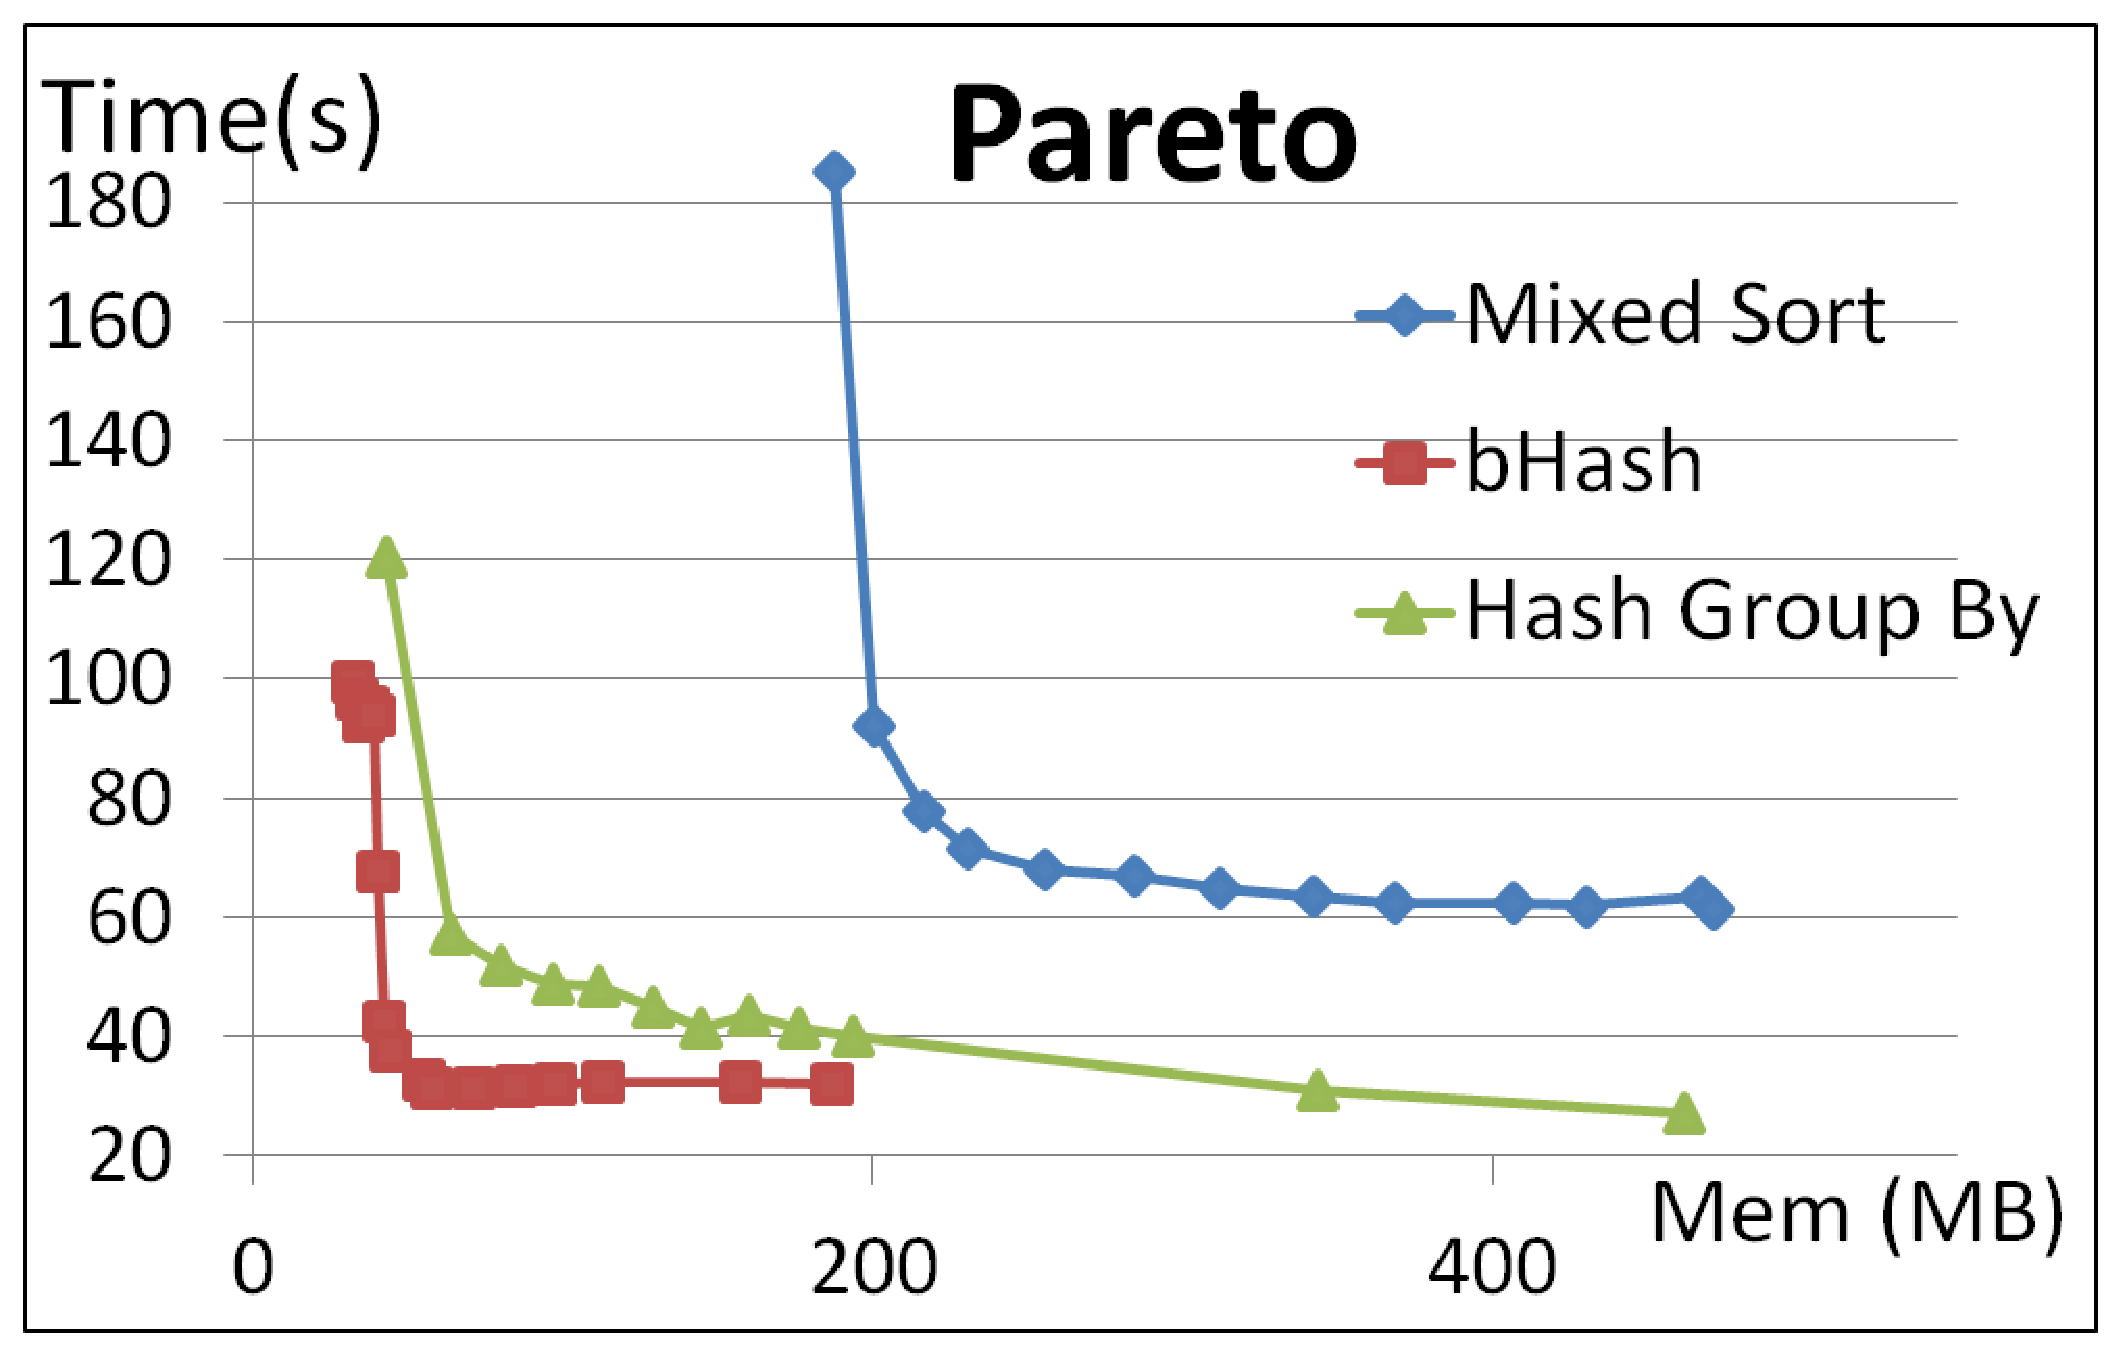
\includegraphics[width = 1.61in]{fig/paretoMemTime.eps}\label{fig:paretoMemTime}}\ \
    % \hspace{2pt}
%    \subfloat[Running time for various file numbers]{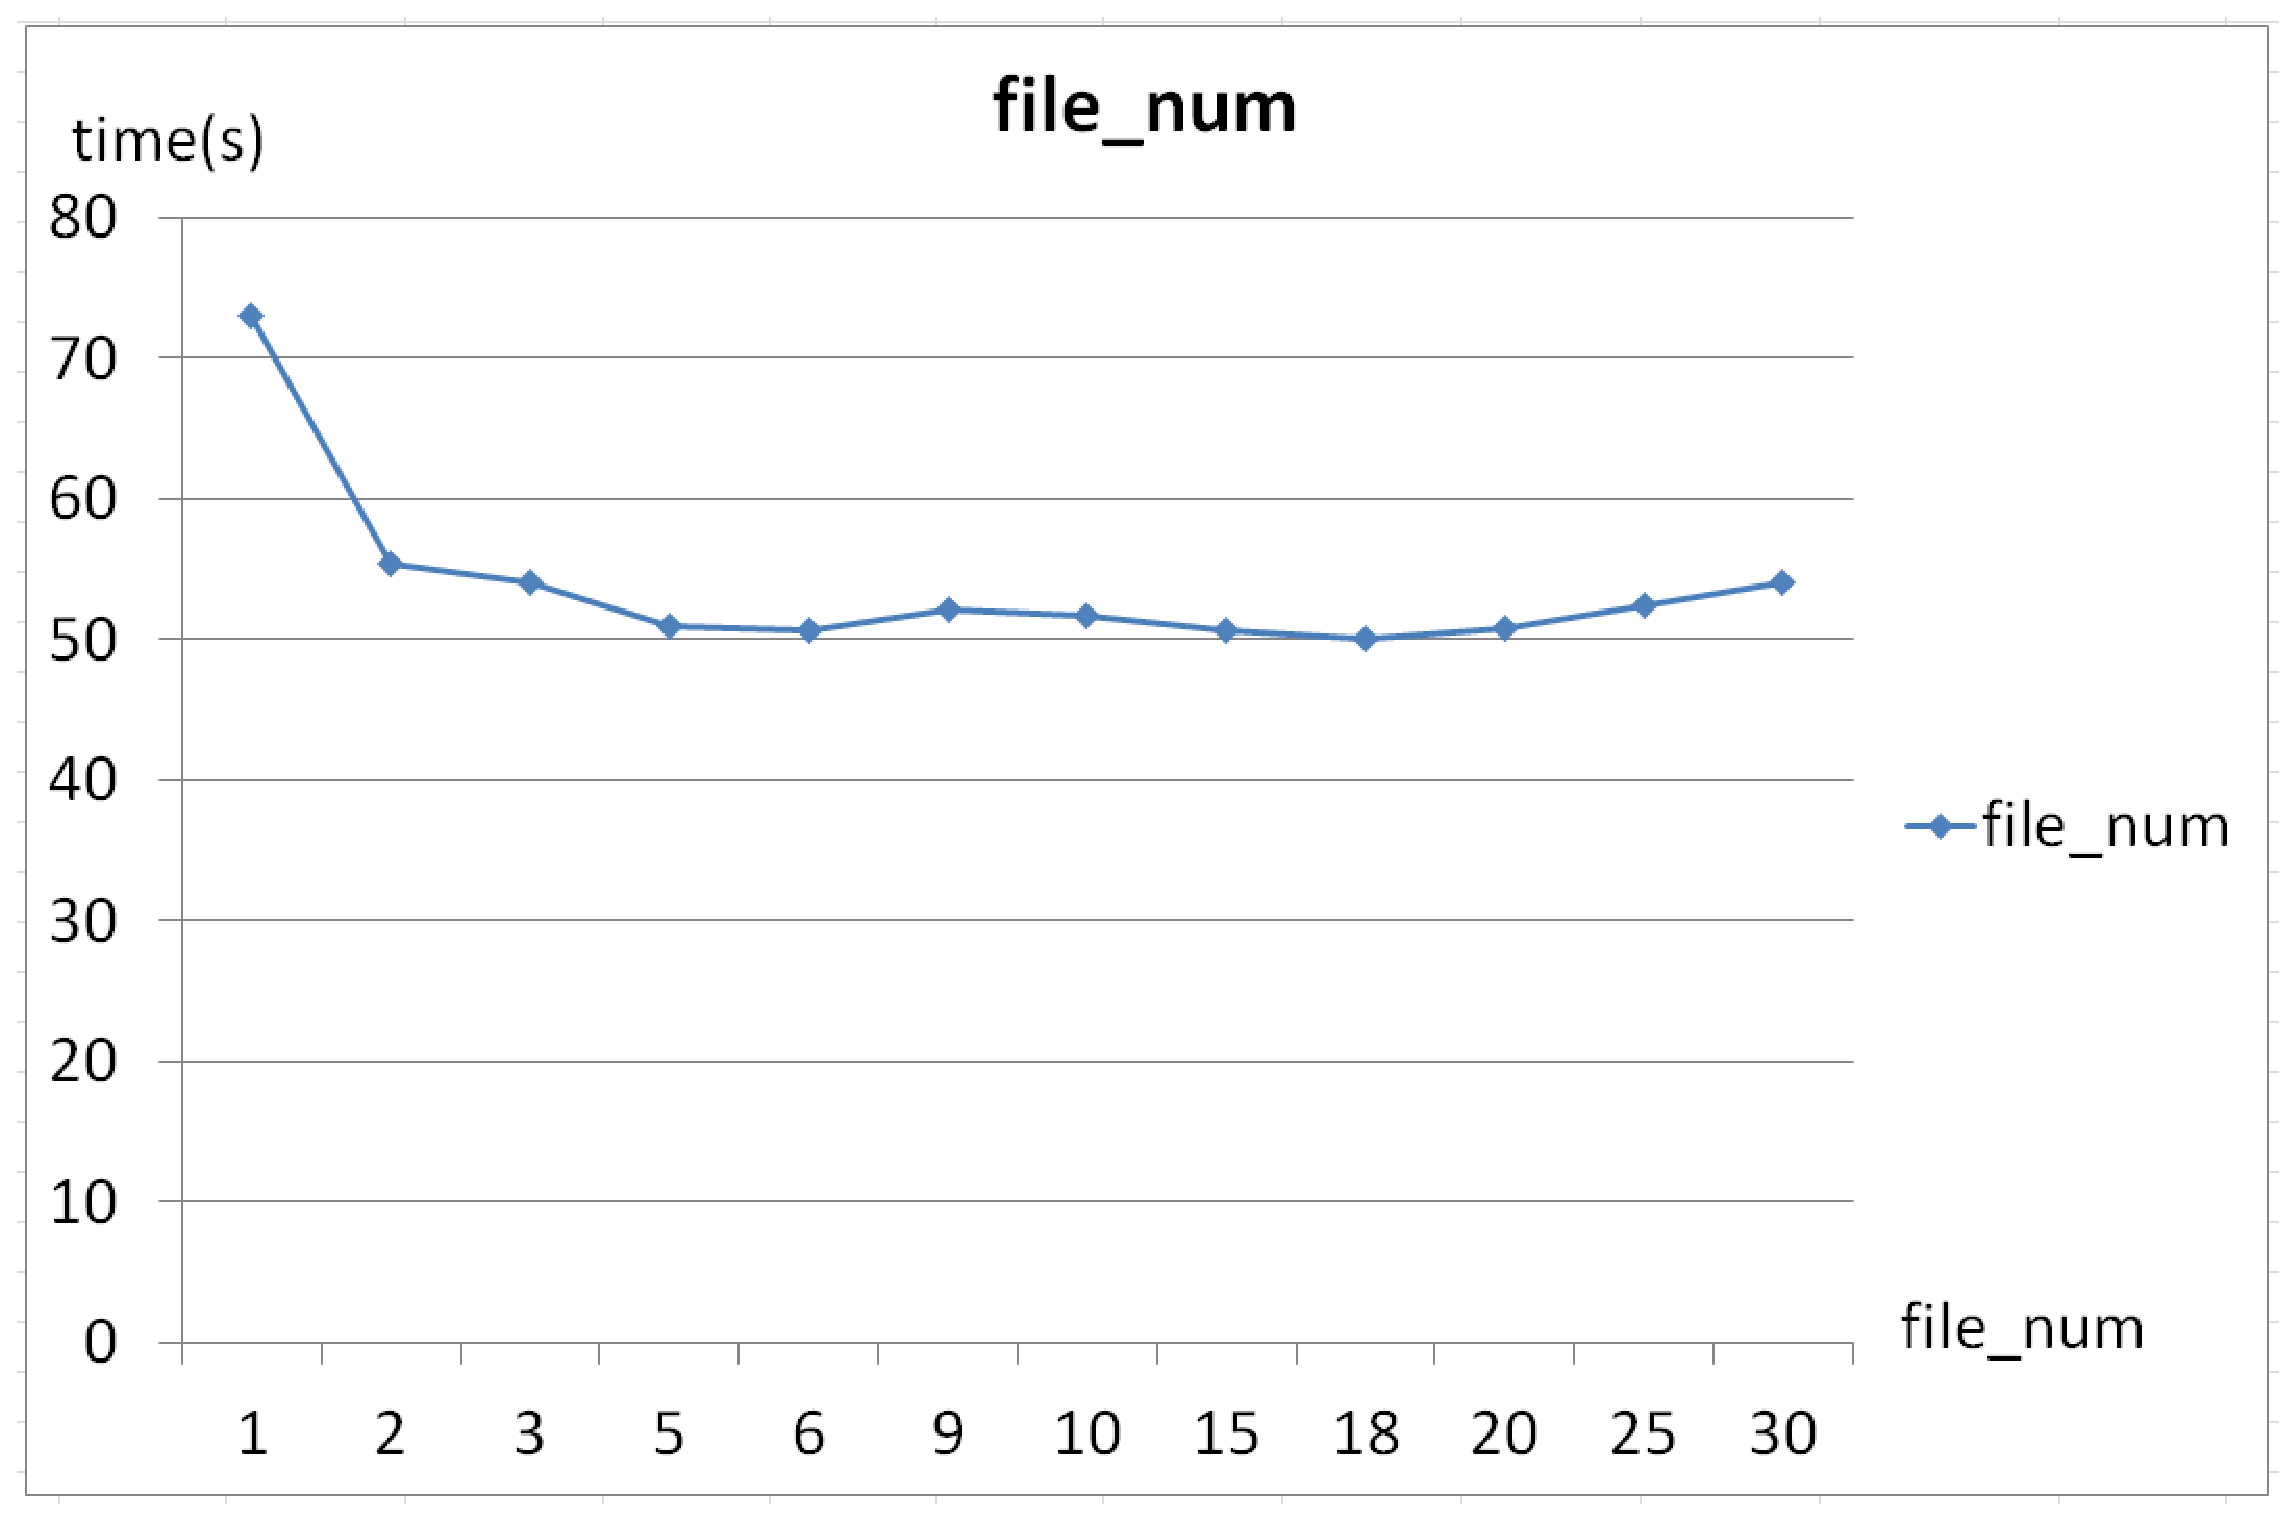
\includegraphics[width = 2in]{filenumTime.eps}\label{fig:buffersizeTime}}\ \
%     \hspace{2pt}
%    \subfloat[Memory usage for various file numbers]{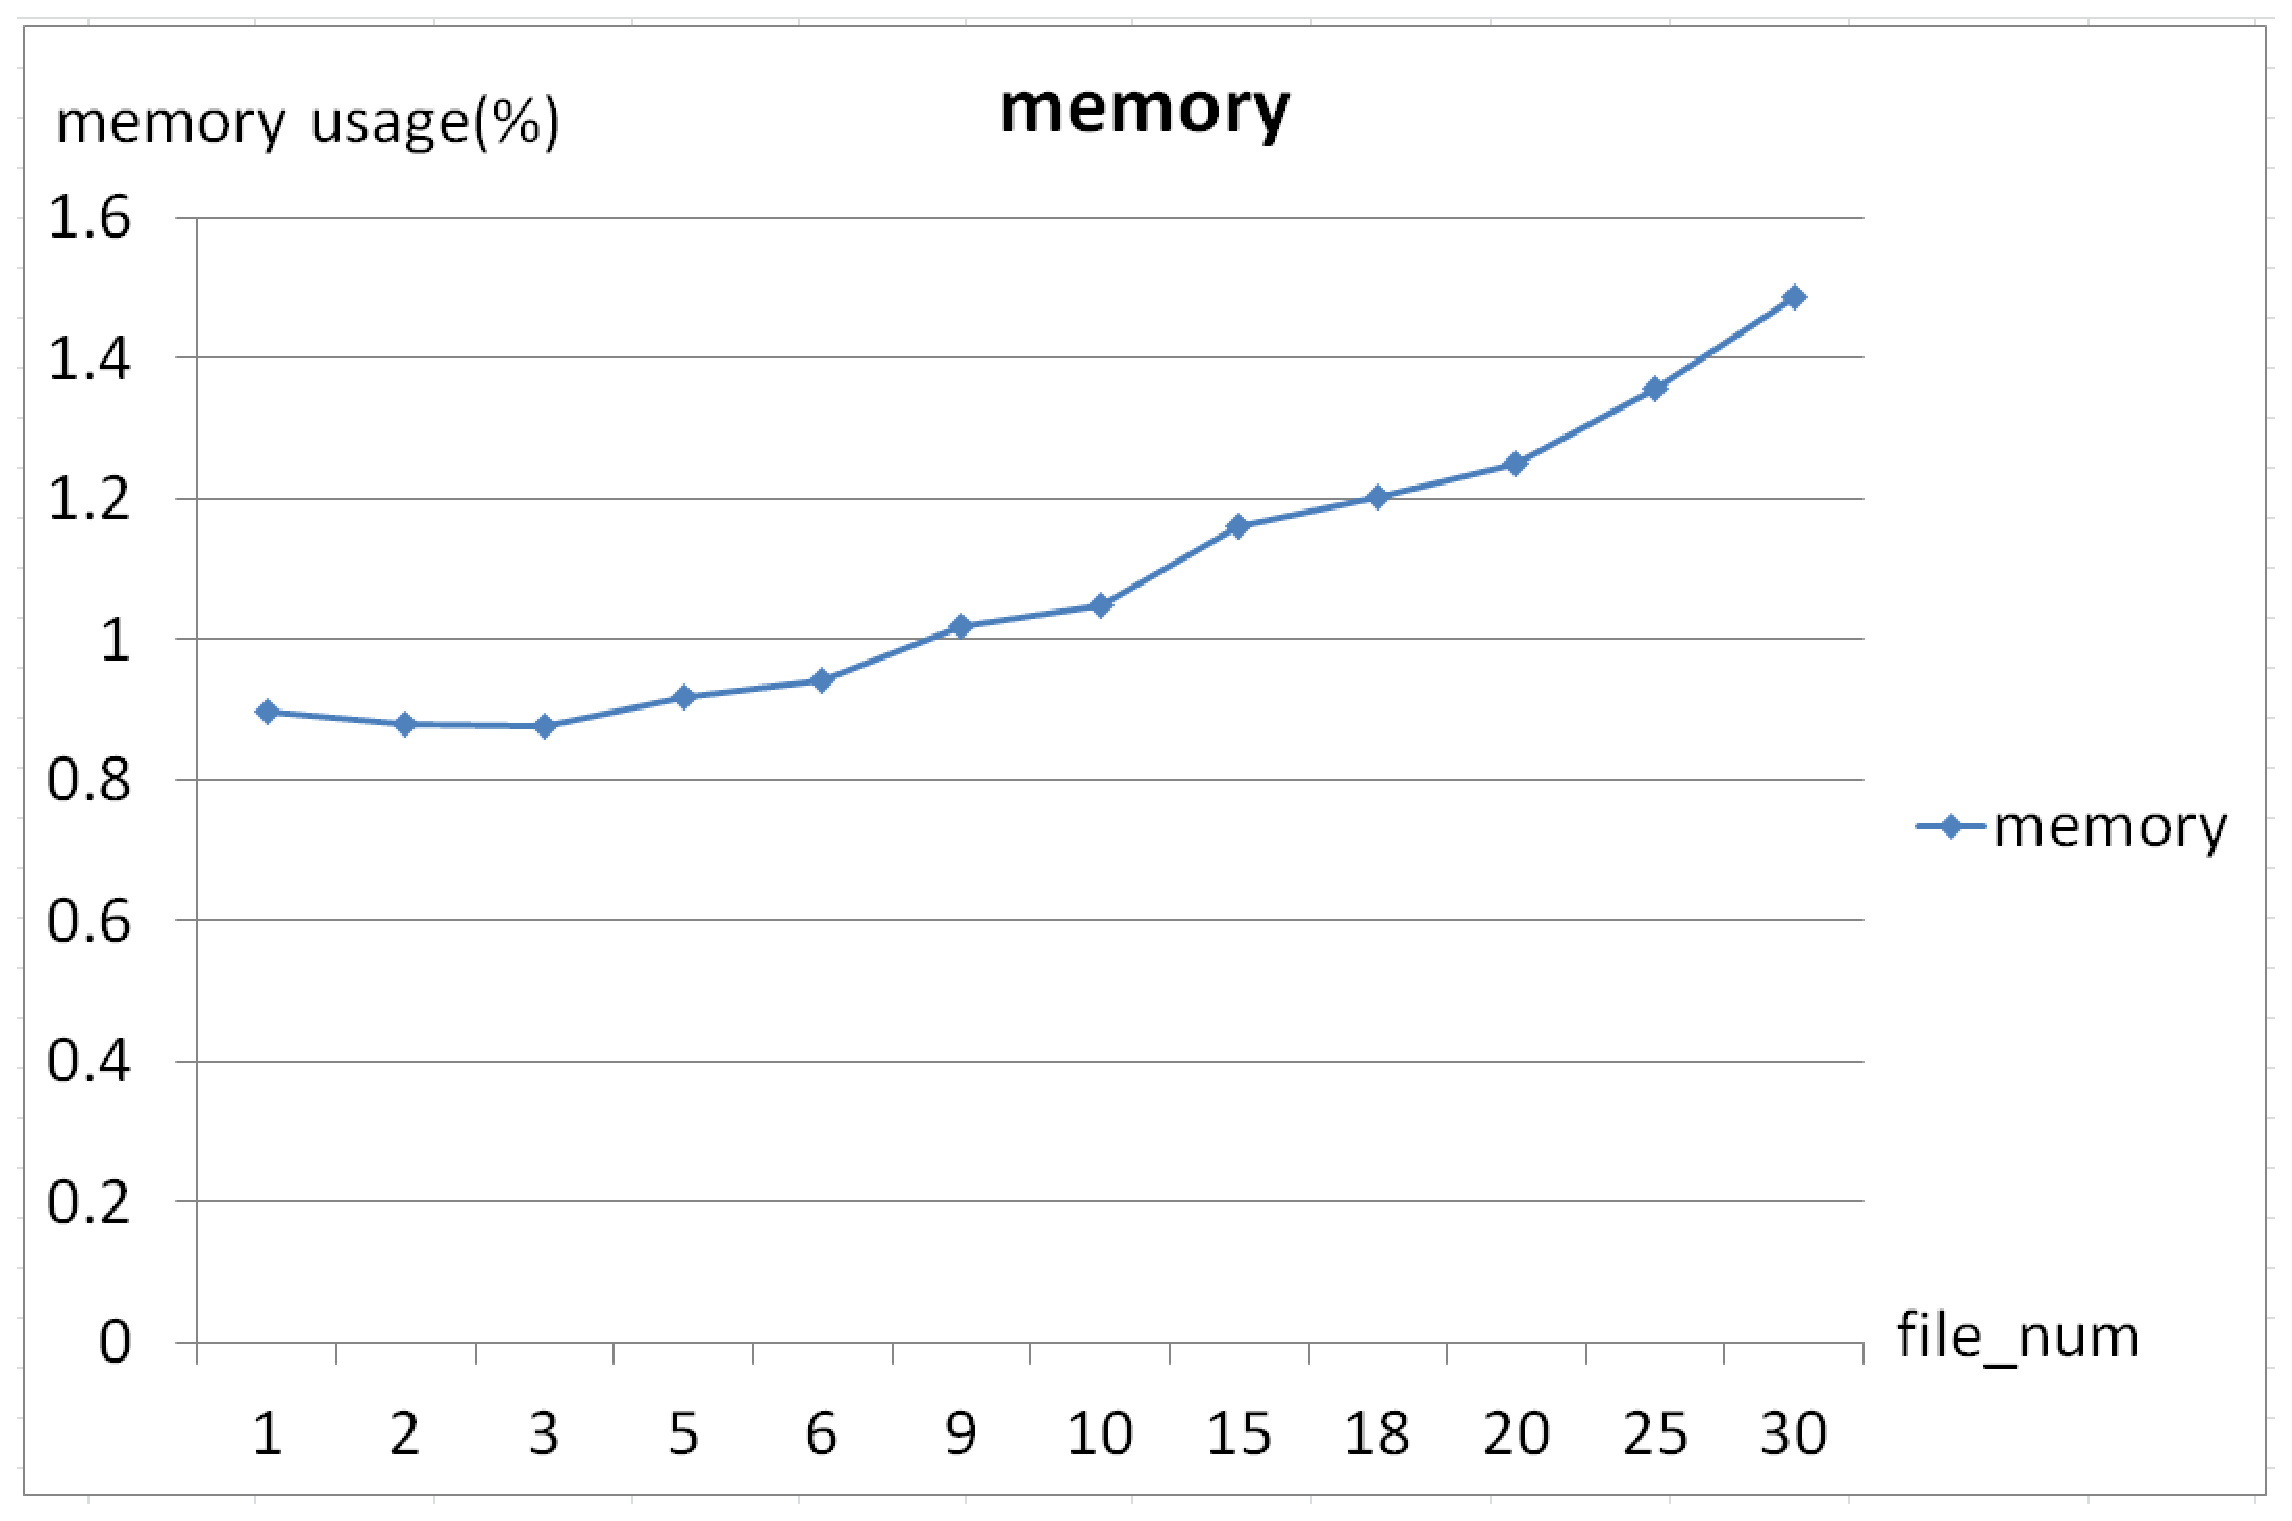
\includegraphics[width = 2in]{filenumMem.eps}\label{fig:buffersizeTime}}\ \
    \caption{Performance comparison on various data sets.}\label{fig:Performance comparison evaluation}
\end{figure*}

\begin{table}
  \caption{Data sets}
  \label{tab:commands}
  \begin{tabular}{ccl}
    \toprule
    dataset &size & illustration\\
    \midrule
    Twitter & 180.4MB& Twitter social network statistics data\\
    Google & 97.2MB & Google web graph data\\
    Wiki	&1.2GB	& Wikipedia access data in one day\\
    Normal	&589.6MB& Normal distributed simulation data\\
    Pareto & 575.4MB & Pareto distributed simulation data\\
    Gama & 594.8MB	& Gama distributed simulation data\\
    \bottomrule
  \end{tabular}
\end{table}

All serial methods were implemented in C++, and compiled with g++ version 4.8.4 in Linux. The experiments were executed on a machine with two quad-core Intel CPUs at 2.67GHz and 32GB RAM.



\subsection{Overall Performance Evaluation}

The following experiments compare bHash against merge-sort and memory-constraint hash. In order to compare these algorithms fairly, we added a buffer for each file in the merge phase of sort grouping. During evaluating the grouping time, we have allotted to all algorithms the same amount of memory. In this experiment, we also investigate the time performance of the three grouping methods with memory usage varying.

Figure 3 (a) compares the grouping time of three methods for different data sets as showed in Table 1 with the same memory size ranging from 0.2\% to 2\%. bHash is consistently faster compared to the other algorithms merge-sort and memory-constraint hash using the same amount of memory. Merge-sort algorithm is the slowest one among the three methods, because there is unnecessary computational overhead in aggregating kv-pairs with merge-sort algorithm as we have analyzed in section \uppercase\expandafter{\romannumeral2}. For the simulation data sets Normal, Pareto and Gama whose size is almost same, merge-sort costs almost the same time, which verifies the feature of no data distribution dependency (has shown in section \uppercase\expandafter{\romannumeral2}). Figure 3 (b) and (c) show the running time acceleration percentage of our bHash compared the existing algorithms: merge-sort and memory-constraint hash respectively using the same amount of memory. The experiment result shows that the processing of various data sets is at least 20\% times faster than merge-sort and even up to 57.8\% times. It speeds up the execution time compared to memory-constraint hash from 4\% to 45\%. What's more, for the long-tailed distributions such as Pareto, our algorithm even achieves 50\% better overall performance than merge-sort but occupies 40\% times less memory and 45\% faster than memory-constraint hash with 39\% times less memory.

Simulation data sets are mainly to evaluate the robustness of our algorithm for grouping data with different distributions especially for skewed data like long-tailed distributions. We generate three representative distributions data, Normal \cite{marsaglia2004evaluating}, Pareto \cite{rootzen2006multivariate} and Gama \cite{minka2002estimating}. The Normal distribution is the most popular data distribution in real world. As figure 3 shows, bHash improves the time performance up to 32.9\% compared to merge-sort and 7.7\% compared to memory-constraint hash. When the data skews seriously, the grouping performance of memory-constraint hash algorithm drops sharply. The running time comparison figure for data set Pareto and Gama shows that the execution time of memory-constraint hash algorithm is almost as much as merge-sort. In contrast to our algorithm, it improves the time performance still obviously, and is 16\% times faster than memory-constraint hash under the data set Gama. For the other data set Pareto, bHash is even 45.8\% times faster than memory-constraint hash. Therefore, memory-constraint hash is not good enough for skewed data.

We make the following analysis to this phenomenon:  Recall to section \uppercase\expandafter{\romannumeral2}, for memory-constraint hash, one or more buckets will be selected to spill to disk when the memory used has reached the threshold. Spilled partitions will be read back to re-aggregate subsequently. The long-tailed distribution makes it more difficult to divide the work data into small uniform portions. For a larger bucket spilled to disk, subsequent reading back and re-aggregating may lead to recursively execute the algorithm many times so that read and write the disk more frequently. The I/O overhead increases sharply. However, bHash performs well. As we know, the long-tailed distribution means that most of kv-pairs are distributed in a few groups. If we have fewer unique groups, the number of entries in the hash table is smaller because the algorithm keep an entry for each group and the memory required is less. Furthermore, if there are more kv-pairs mapped to the same group, the buffered kv-pairs for a group in grouping buffer will be more between two flush operation, which improves the data locality. Therefore, our algorithm is able to efficiently aggregate skewed data compared to other algorithms.

The next experiment investigates the scalability of our method. Figure 4 shows the grouping times in seconds of these algorithms with the memory available increasing. we list experimental results on some representative data sets since experimental results on other data sets are similar. On the whole, our algorithm is almost distributed lower than other algorithms in Figure 4, e.g., in the case of the same memory consumption, our algorithm performs faster and takes up less memory under the same time cost. For merge-sort and memory-constraint hash, the execution time continues to decline with the memory available increases constantly. For merge-sort, when the memory is large enough to sort kv-pairs in memory completely, the performance is no longer enhanced and memory consumption is six times than bHash(as shown in Figure 4 (b) (c) (d)). Compared to our method, memory-constraint hash need two times memory for Wiki and four times memory for Twitter to archive the same time performance. For long-tailed distributions, bHash even can save up to six times more memory compared to memory-constraint hash. For the Wiki data set, bHash curve starts on a higher memory usage as shown in Figure 4 (a), which mainly because it needs certain memory to store offset for each group. Recall to section \uppercase\expandafter{\romannumeral3}, two buffers are applied to reduce disk I/O, the buffer size is almost set to zero in the condition of the maximum execution time in Figure 4 and we increase memory consumption by increasing the buffer size in the experiment. As seen from Figure 4, bHash can achieve the best performance from the worst execution time by increasing a little more buffer. what's more, a larger memory only improves the time performance very little and waste space, which proves that our algorithm can achieve perfect performance with less memory.

In general, bHash performs from 20\% to 57.8\% times faster than merge-sort and faster than memory-constraint hash up to 45\% times in condition of using the same memory. For the long-tailed distributions such as Pareto, our algorithm even achieves 50\% better overall performance than merge-sort but occupies 40\% times less memory and 45\% faster than memory-constraint hash in the case of using 39\% times less memory. Our method can save memory up to from two to six times compared memory-constraint hash and performs well both in time performance and memory consumption.

\subsection{Parameters Evaluation}
%For these reasons using bHash, the processing of various data sets is at least 20\% times faster than Mixed Sort algorithm and even up to 57.8\% times. On the other hand, bHash speeds up the execution time compared to Hash Group By up to 45\%.

%parameterEvaluation
\begin{figure*}%figure 8
    \centering
    \subfloat[Time and memory on bucket number ]{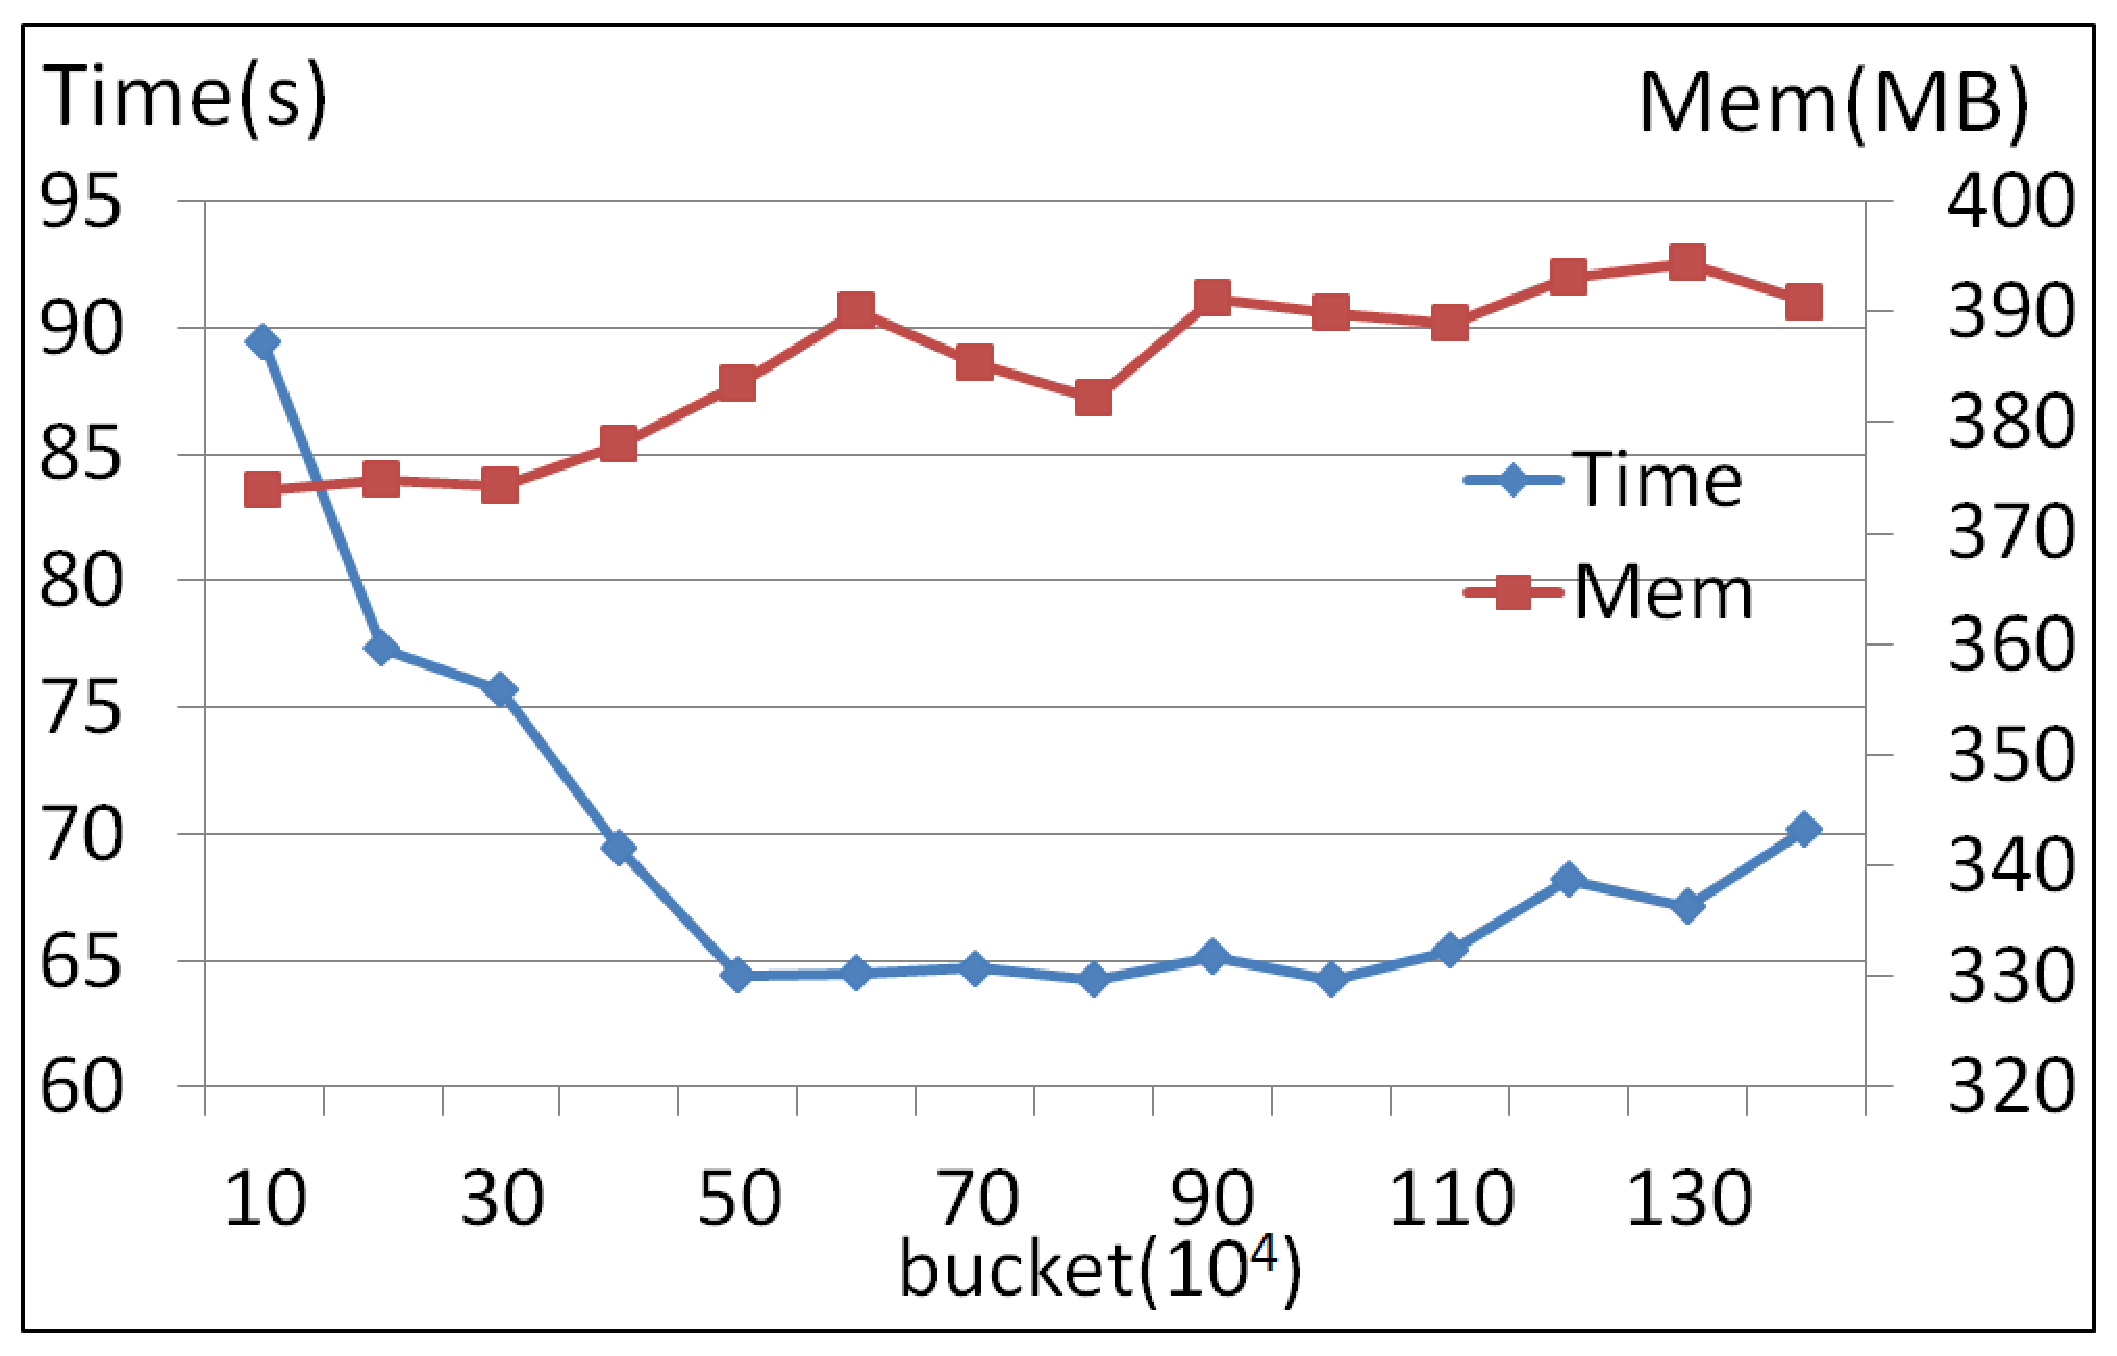
\includegraphics[width = 2in]{fig/bucketMemTime.eps}\label{fig:bucketMemTime}}\ \
    \hspace{1pt}
    \subfloat[Time and memory on grouping buffer]{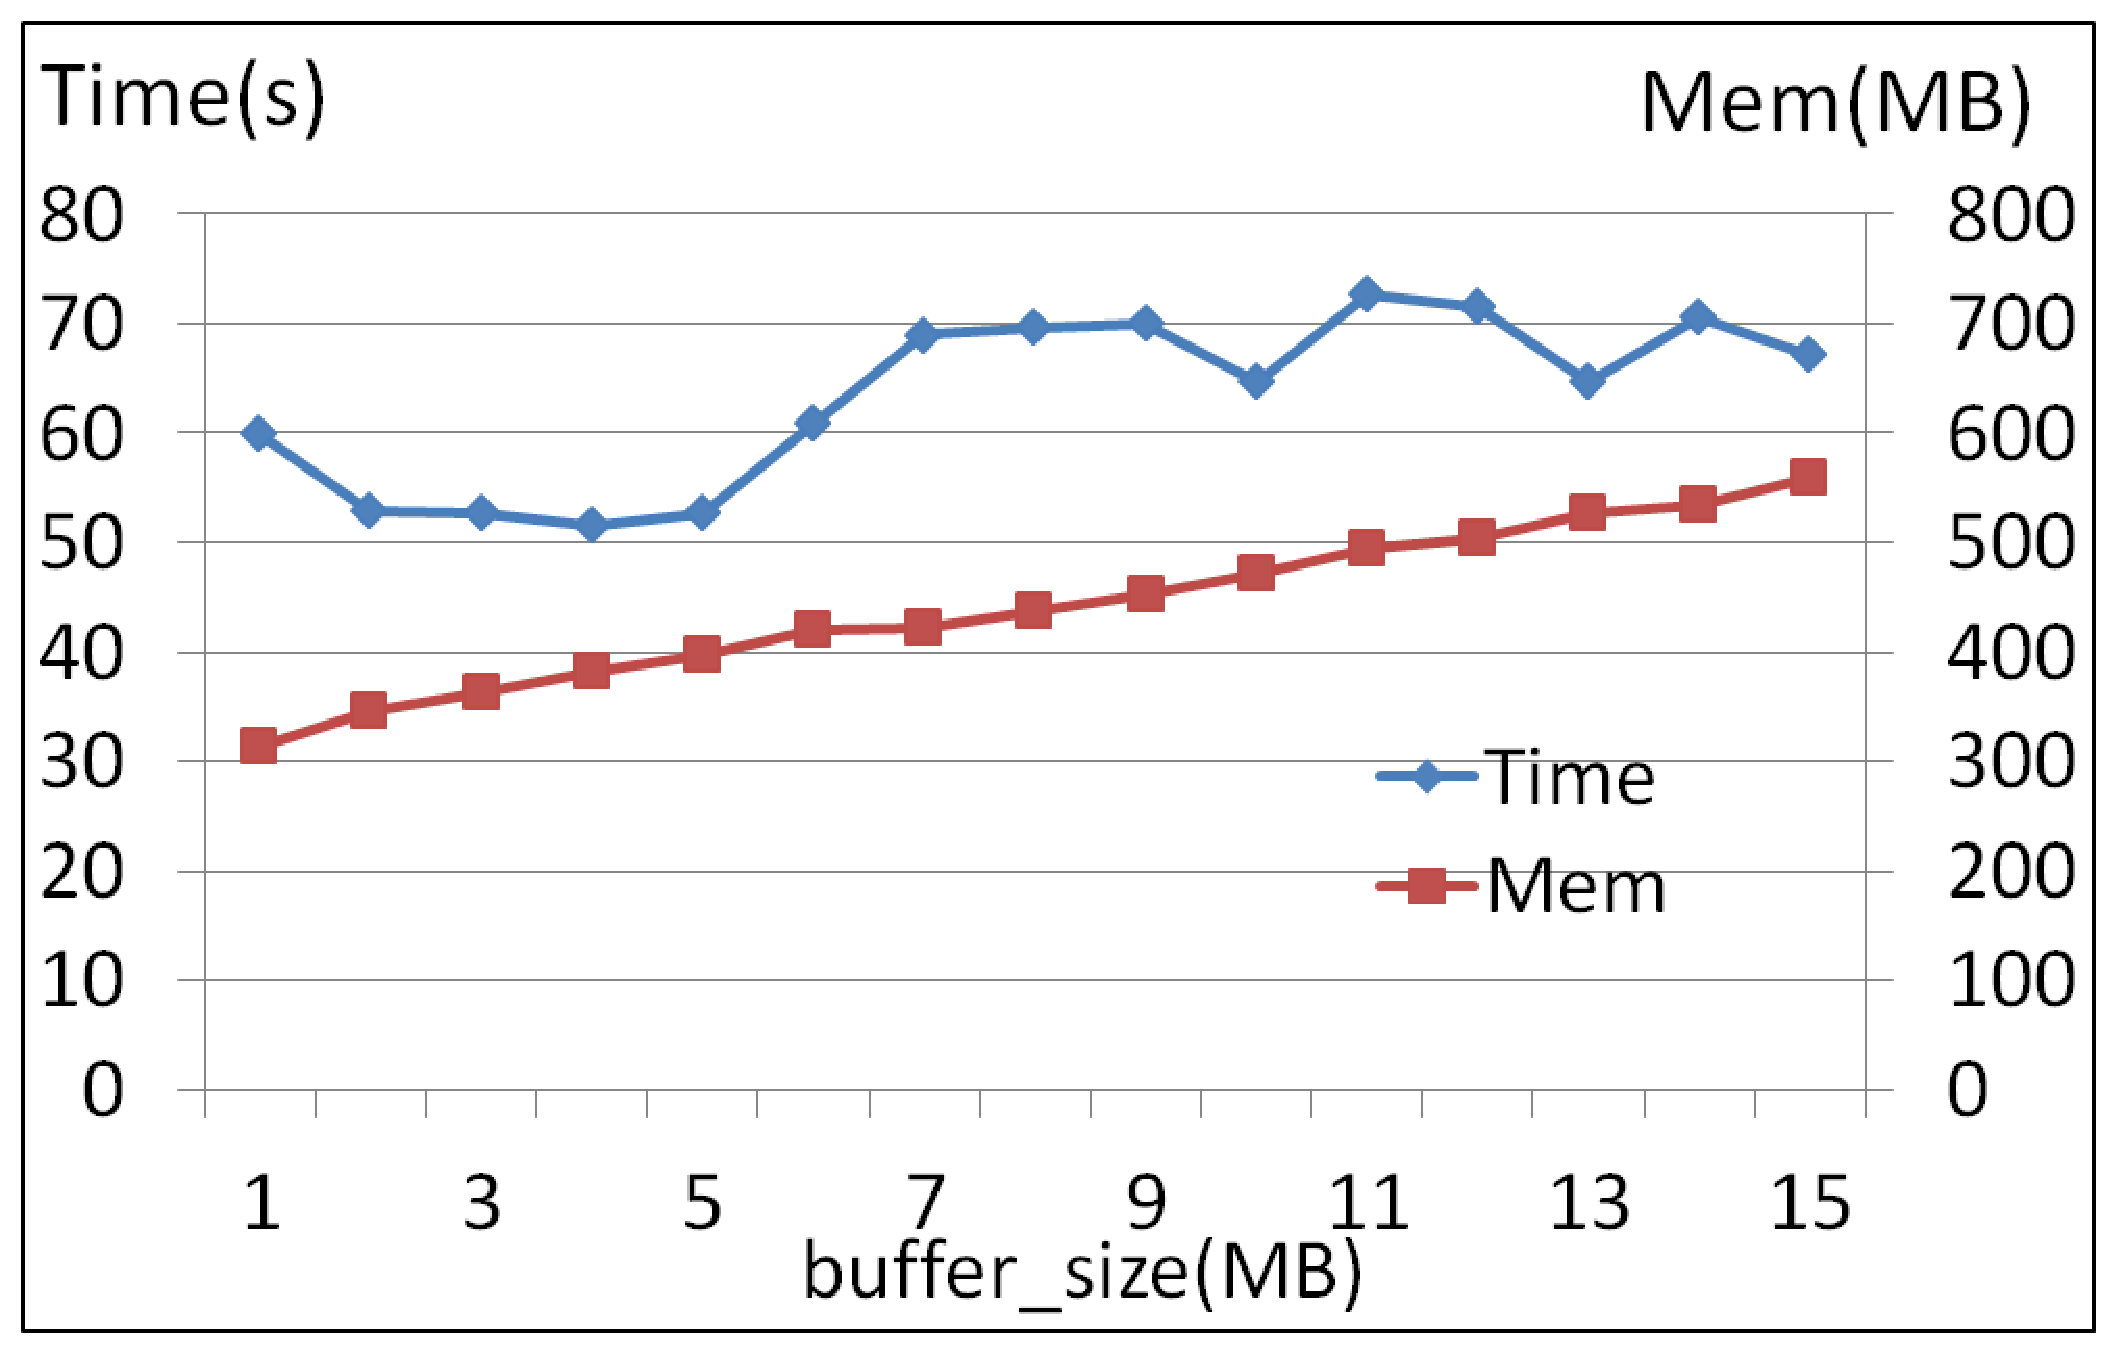
\includegraphics[width = 2in]{fig/buffersizeMemTime.eps}\label{fig:buffersizeMemTime}}\ \
    \hspace{1pt}
    \subfloat[Time and memory on sub file number]{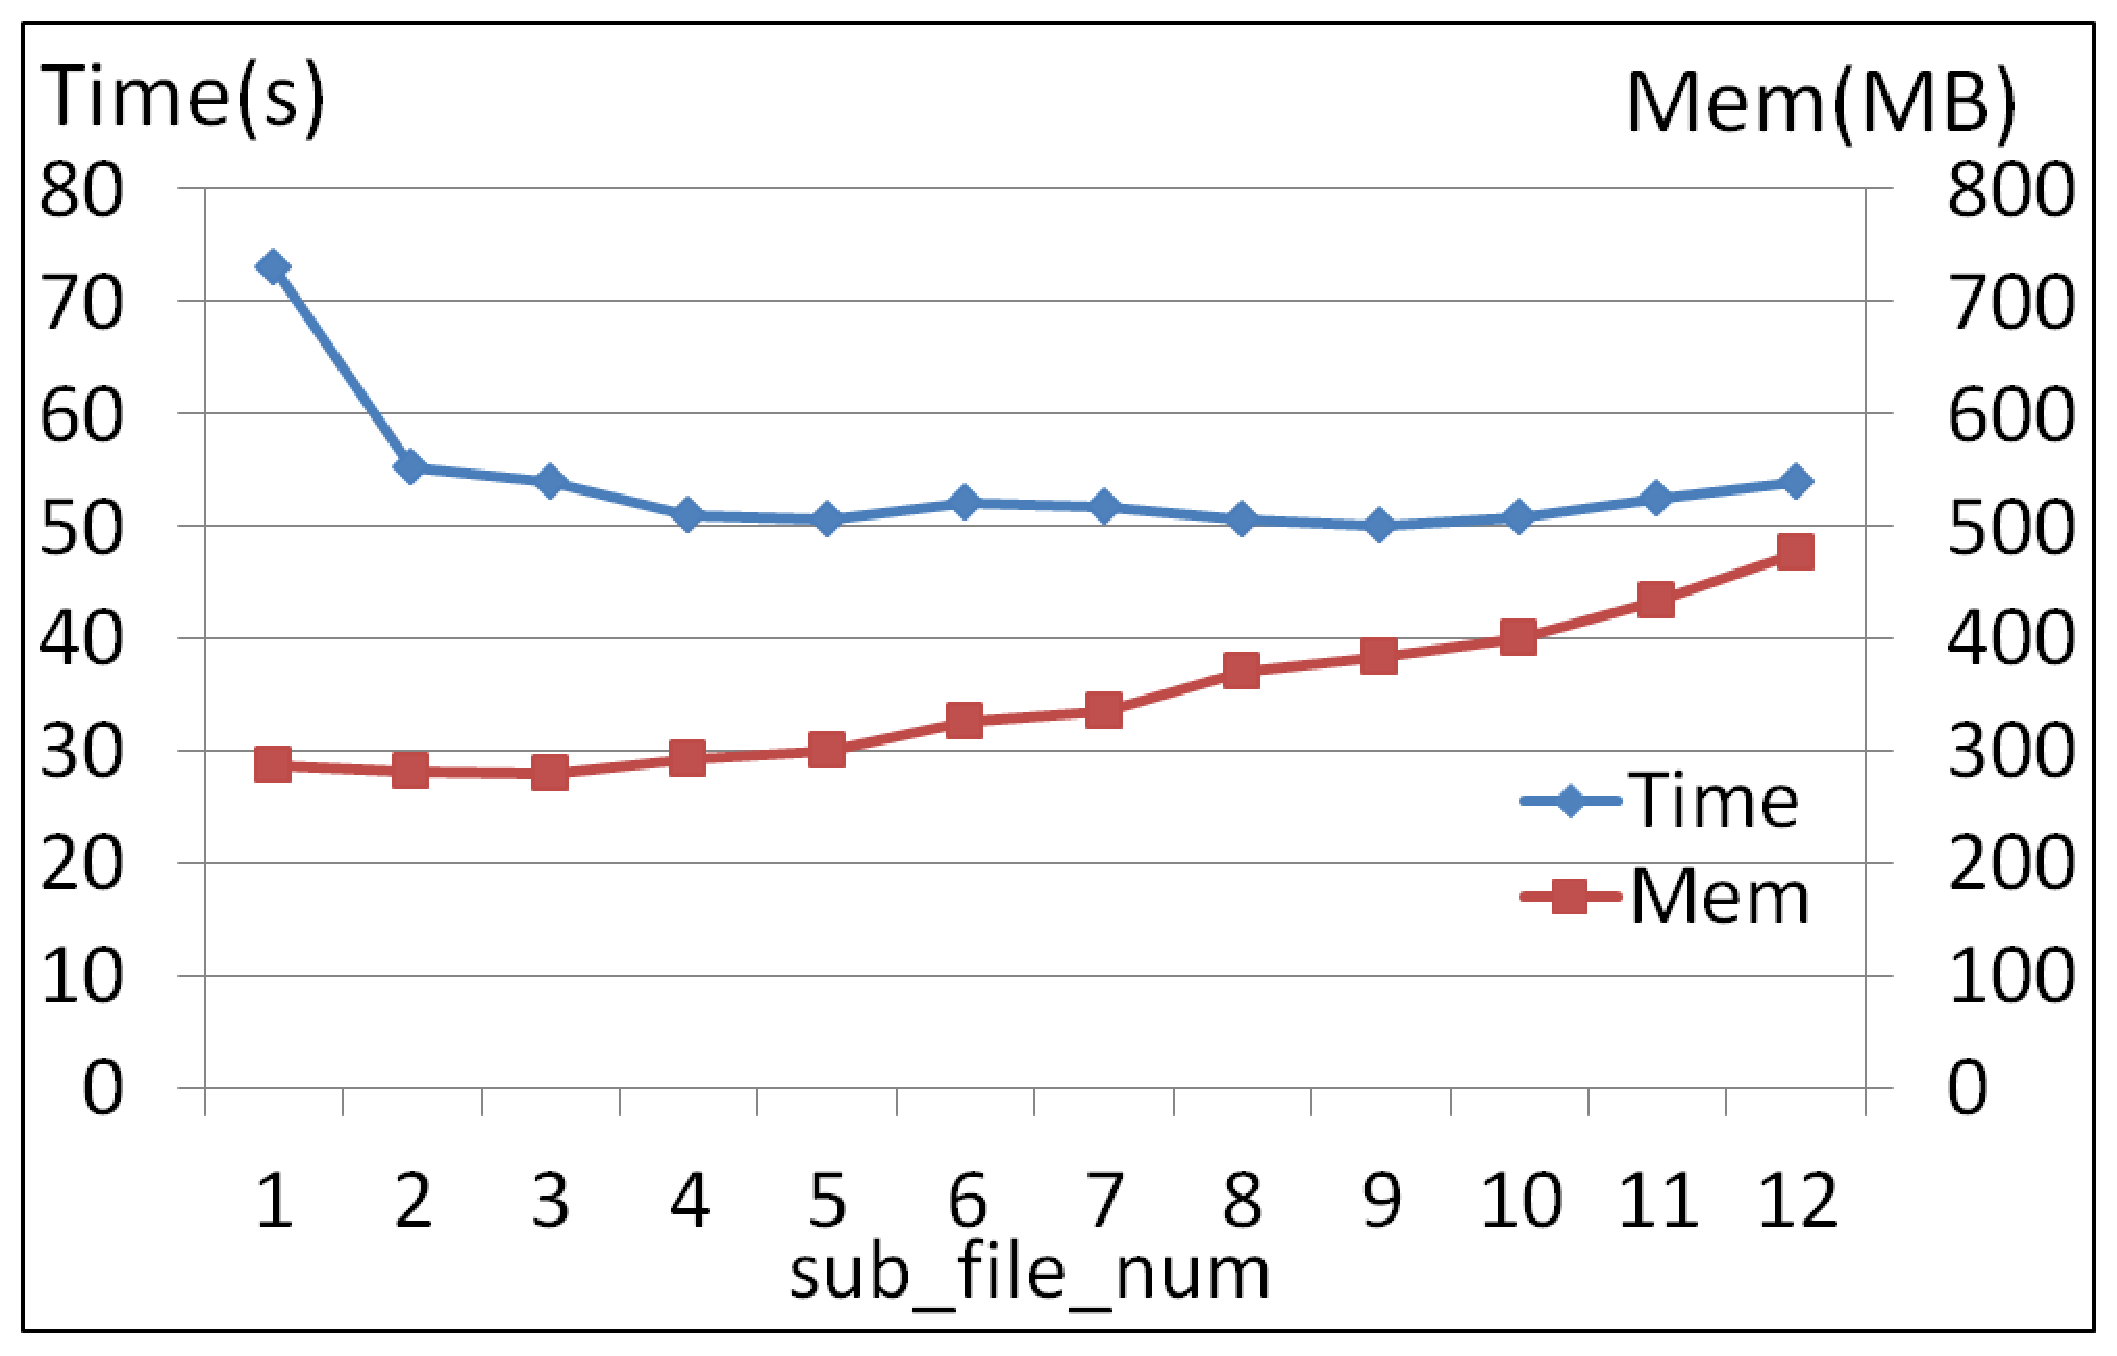
\includegraphics[width = 2in]{fig/filenumMemTime.eps}\label{fig:filenumMemTime}}\ \
    \caption{Parameters evaluation.}\label{fig:Parameters evaluation}
\end{figure*}

\begin{figure*}%figure 9
    \centering
    \subfloat[Runtime ]{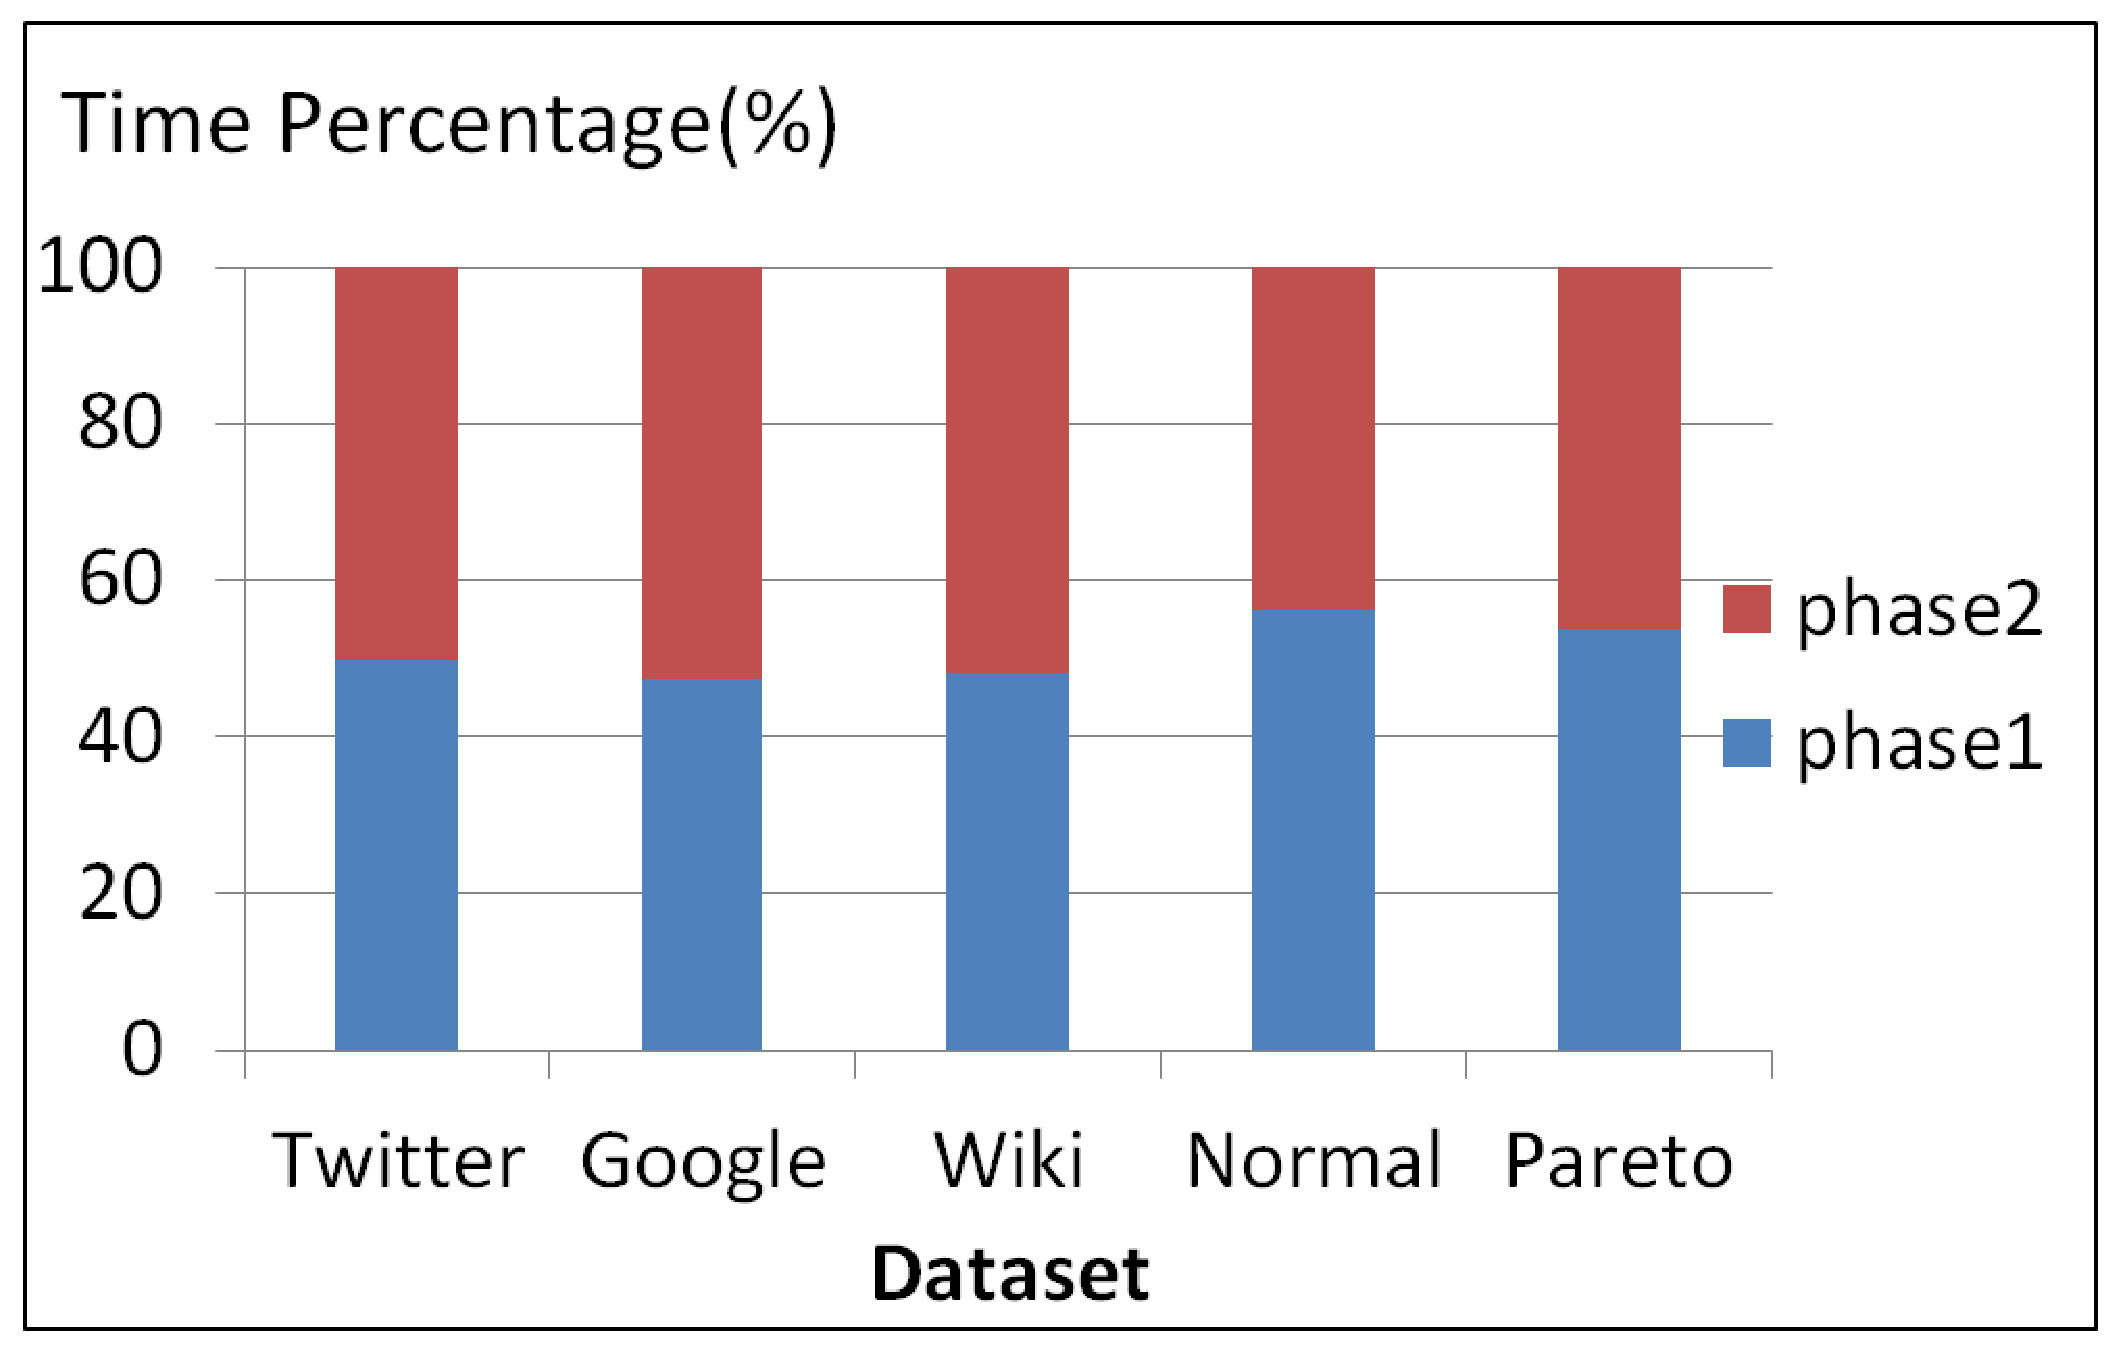
\includegraphics[width = 2in]{fig/TimePercentage.eps}\label{fig:TimePercentage}}\ \
    \hspace{1pt}
    \subfloat[Memory consumption]{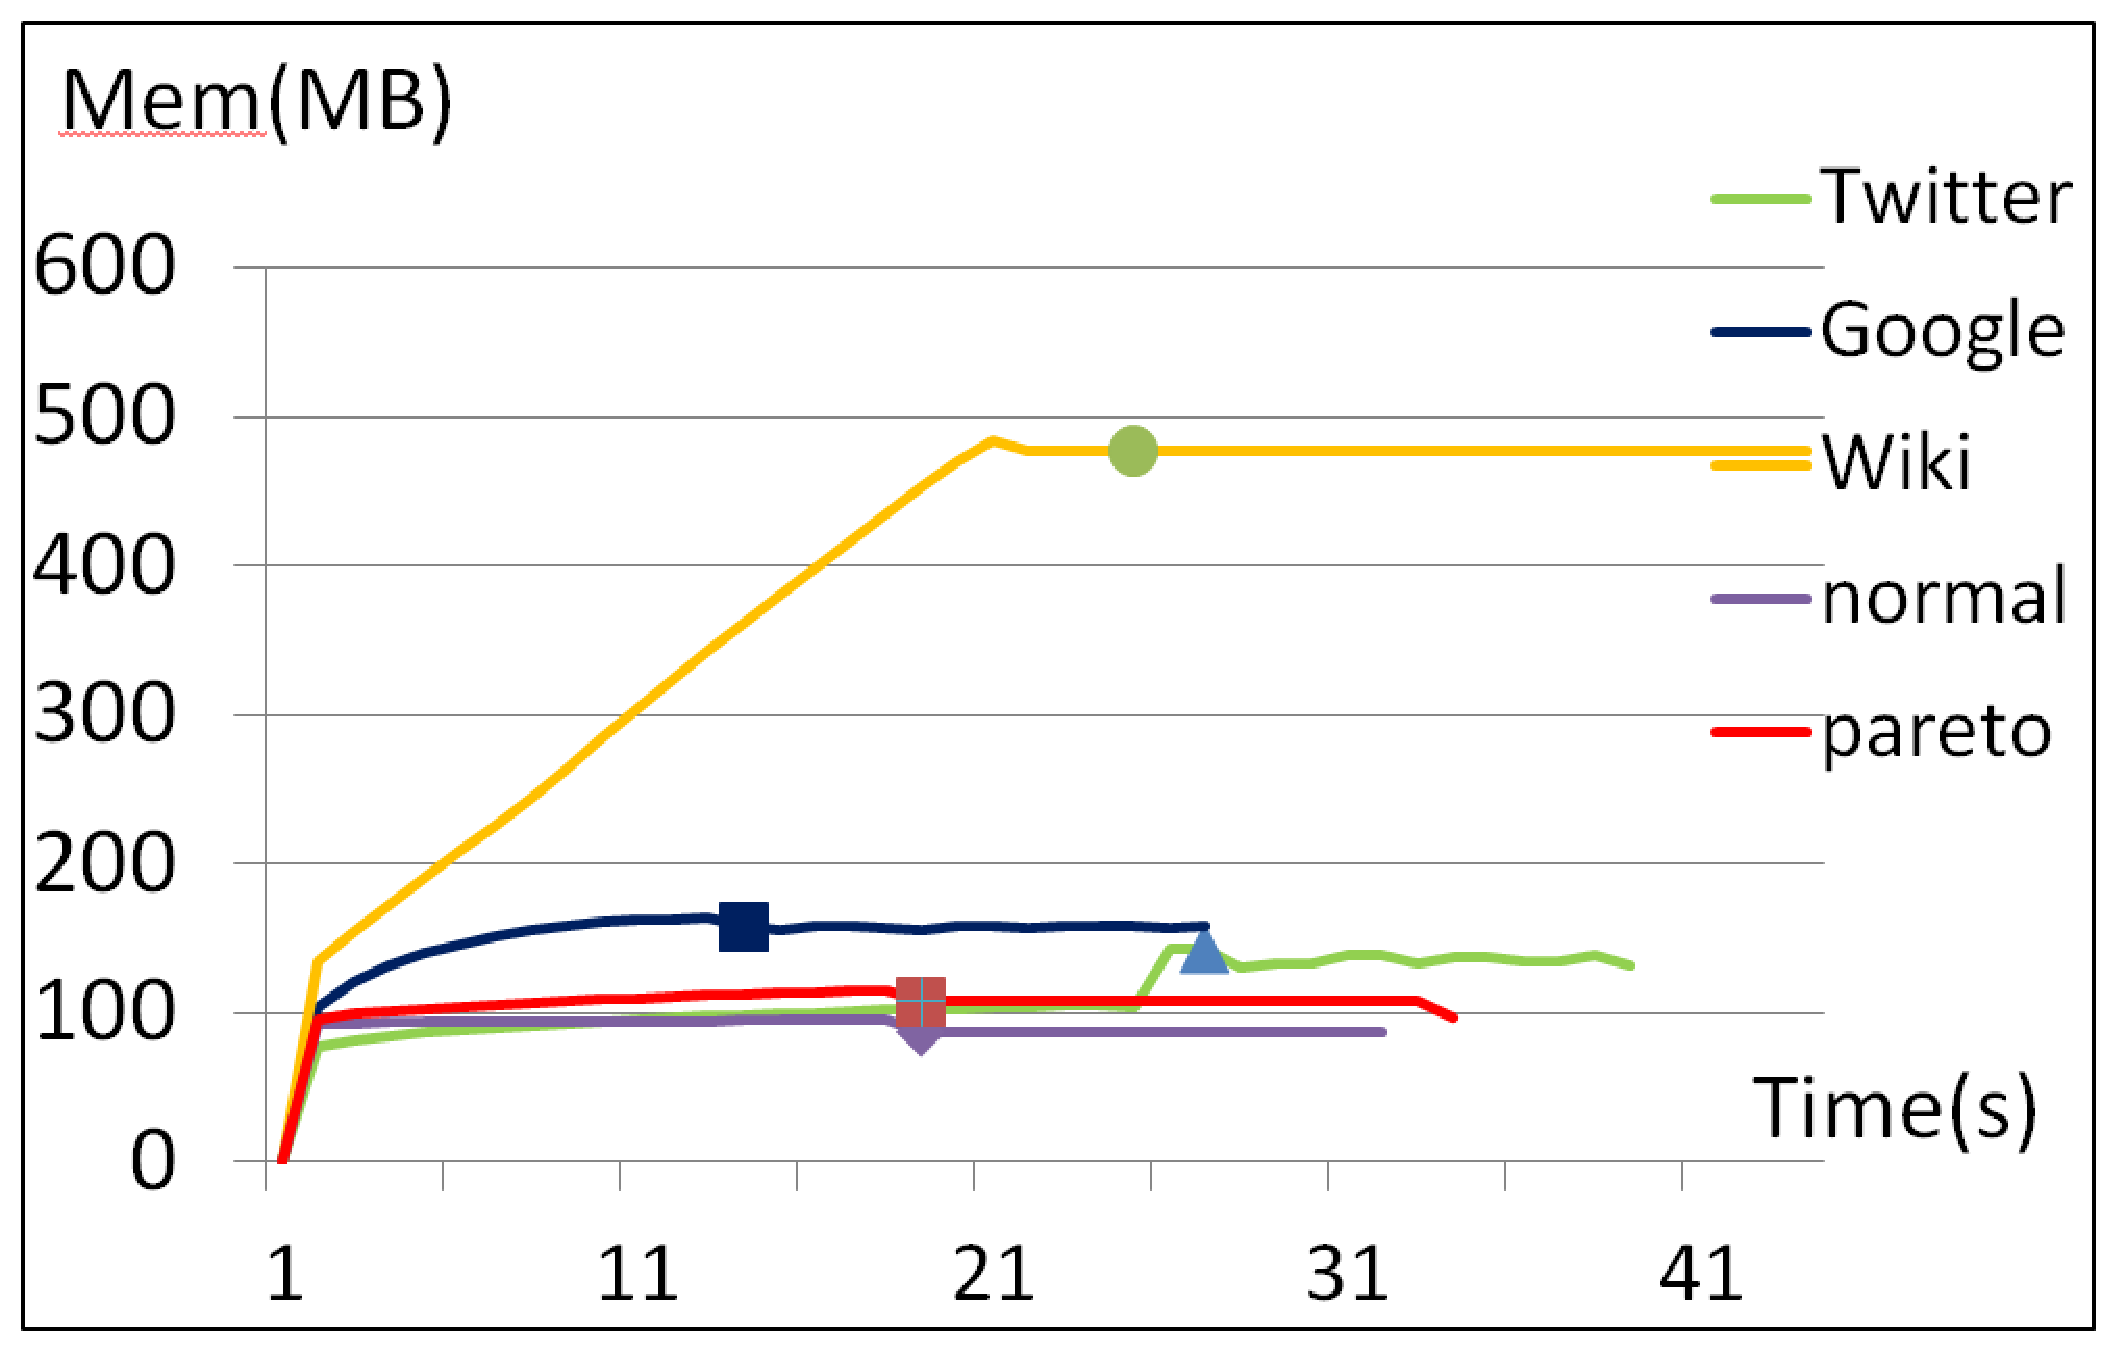
\includegraphics[width = 2in]{fig/MemPhase.eps}\label{fig:MemPhase}}\ \
    \caption{Runtime and memory consumption comparisons between two phases.}\label{fig:Phase evaluation}
\end{figure*}


In the work, we also evaluate the impact on different parameters of bHash. The number of hash buckets is set to from 500,000 to 900,000, which makes the algorithm perform best for all data sets. The number of sub files has little effect on the performance as long as greater than or equal to two. The buffer for partial grouping results is not as bigger as better. Interestingly, the execution time using a relatively smaller buffer will be shorter, which is determined by the internal mechanism of bHash. We have experimentally evaluated on various data sets in Table 1 and theoretically analyzed the effects of these parameters on the algorithm including the number of hash buckets, the size of buffer and the number of sub files. We take the representative experiment result on the maximum data set Wiki as an example. Figure 5 shows the strong scalability results for the algorithm.

\textbf{The number of buckets}. Recall from Section \uppercase\expandafter{\romannumeral3} that horizontally partitioning in bHash that splits the source file into multiple sub files to amortize the I/O cost. Figure 5 (a) compares the effect of using hash buckets of different sizes. From 100,000 to 500,000, bHash executes faster with the increase in the number of hash buckets. When the number of hash buckets is too small, one query may cost longer time because there will be more grouping entries mapped to the same bucket. In practice, the number is set to exceeding 500,000, which can archive efficient result. Too many buckets will occupy more memory as depicted in figure 5 (a). The experiment results show that the range from 500,000 to 900,000 is the best size to balance the time cost and space cost.

\textbf{Buffer size}. The next experiment shows the effect of the grouping buffer size. Recall from file filling phase in section \uppercase\expandafter{\romannumeral3} that as more grouping kv-pairs are generated, bHash uses the buffer to buffer grouping data of different groups to reduce the I/O cost because of seeking disk frequently. Figure 5 (b) compares the performance of different buffer size. Note that using a oversized buffer is not a good alternative to bHash. For example, 4M is 12\% faster than 1M for the buffer size, but it is 24\% slower than 8M for Wiki data set. Recall from the file filling in Algorithm 1, we deal with one spill at a time, the kv-pairs buffered are almost wrote to the same grouping file. If the buffer size is too large, the data buffered in buffer may involve multiple files. When one flush is triggered, kv-pairs to be flushed may belong to several files, so the seek operations will skip from a file to another file and skip back again in the next time. In order to reduce the unnecessary I/O cost, a larger buffer is not required. In our experiments, as long as the buffer size is smaller than or equals to the size of a sub file, the profits gained is the biggest no matter the time performance or the memory usage. For sub-file buffer, the effect of this parameter on performance is little and easy to understand. bHash is sufficient as long as the sub-file buffer size is set greater than or equal to fifty thousand in experiments.

\textbf{The number of sub files}. The following experiments compare the grouping time for the Wiki data set with sub file number ranging from 1 to 30 as depicted in Figure 5 (c). bHash with splitting is 24\% times faster compared to one sub file. However, when the number of sub files is larger than two, running time has not been significantly improved. Recall from Section \uppercase\expandafter{\romannumeral3}, we have allotted a buffer for each sub file to buffer the partitioned kv-pairs, thus the memory allocated continues to rise with the file number increasing as depicted in Figure 5 (c). Therefore, it is worth noting that increase the number of partition files excessively. The number of partition files is set to 10 is sufficient in all experiments.
\subsection{Phase Evaluation}
In this subsection, we discuss the impact and interrelated factor on the Statistics Collection phase and the File Filling phase. Figure \ref{fig:Phase evaluation} shows the time percentage and memory consumption on each of the two phases. Statistics collection phase studies the global knowledge of group size information and generates a offset table that contains $\langle group key, file position\rangle$s. File Filling phase writes out kv-pairs to certain file positions according to the offset table.

Figure \ref{fig:TimePercentage} shows the time percentage of the two phases on different data sets. We can notice that, for both Statistics Collection phase and File Filling phase, the time percentage is close to 50\%. Since bHash needs one pass of data in each phase and the main cost is from disk read/write, the time consumption of the two phases is almost equal.

We also compare the memory usage for the two phases on various data sets as depicted in Figure \ref{fig:MemPhase}. The mark point on each line separates the two phases and the left(right) side indicates Statistics Collection (File Filling) phase. The memory usage increases over time gradually in phase 1, which is under expected because the number of groups increases when processing more input. 



\section{Conclusions}

Grouping key value pairs are essential for many practical applications that include MapReduce, SQL Hash Group By, etc. The volume of such data increases rapidly, therefore, it is essential to improve fast key value grouping methods. In this paper we proposed bHash, a method that supports very long records, large data sets and works efficiently even if the data distribution is skewed  and is easily implemented. Extensive experimental evaluation with real data sets revealed that our method is much more efficient than existing ones in terms of speed and computational resources. bHash performs 20\%~57.8\% times faster than merge-sort and faster than memory-constraint hash up to 45\% times in condition of using the same memory. For the long-tailed distributions such as Pareto, our algorithm even achieves 50\% better overall performance than merge-sort but occupies 40\% times less memory and 45\% faster than memory-constraint hash in the case of using 39\% times less memory. Our method can save memory up to from two to six times compared memory-constraint hash and performs well both in time performance and memory consumption.

This work is part of a large project that aims to develop an engine for grouping and processing of massive data. We are currently working on scaling our method to the distributed computing framework. As we know, stand-alone aggregating key value pairs of different groups is applied to both map phase and reduce phase in MapReduce independently. So bHash is easily parallelizable. We are also focusing on the parallel processing various types of grouping using the bHash.



% The very first letter is a 2 line initial drop letter followed
% by the rest of the first word in caps.
%
% form to use if the first word consists of a single letter:
% \IEEEPARstart{A}{demo} file is ....
%
% form to use if you need the single drop letter followed by
% normal text (unknown if ever used by the IEEE):
% \IEEEPARstart{A}{}demo file is ....
%
% Some journals put the first two words in caps:
% \IEEEPARstart{T}{his demo} file is ....
%
% Here we have the typical use of a "T" for an initial drop letter
% and "HIS" in caps to complete the first word.
%\IEEEPARstart{T}{his} demo file is intended to serve as a ``starter file''
%for IEEE \textsc{Transactions on Magnetics} journal papers produced under \LaTeX\ using
%IEEEtran.cls version 1.8b and later.
% You must have at least 2 lines in the paragraph with the drop letter
% (should never be an issue)
%I wish you the best of success.

%\hfill mds

%\hfill August 26, 2015



% needed in second column of first page if using \IEEEpubid
%\IEEEpubidadjcol



% An example of a floating figure using the graphicx package.
% Note that \label must occur AFTER (or within) \caption.
% For figures, \caption should occur after the \includegraphics.
% Note that IEEEtran v1.7 and later has special internal code that
% is designed to preserve the operation of \label within \caption
% even when the captionsoff option is in effect. However, because
% of issues like this, it may be the safest practice to put all your
% \label just after \caption rather than within \caption{}.
%
% Reminder: the "draftcls" or "draftclsnofoot", not "draft", class
% option should be used if it is desired that the figures are to be
% displayed while in draft mode.
%
%\begin{figure}[!t]
%\centering
%\includegraphics[width=2.5in]{myfigure}
% where an .eps filename suffix will be assumed under latex,
% and a .pdf suffix will be assumed for pdflatex; or what has been declared
% via \DeclareGraphicsExtensions.
%\caption{Simulation results for the network.}
%\label{fig_sim}
%\end{figure}

% Note that the IEEE typically puts floats only at the top, even when this
% results in a large percentage of a column being occupied by floats.


% An example of a double column floating figure using two subfigures.
% (The subfig.sty package must be loaded for this to work.)
% The subfigure \label commands are set within each subfloat command,
% and the \label for the overall figure must come after \caption.
% \hfil is used as a separator to get equal spacing.
% Watch out that the combined width of all the subfigures on a
% line do not exceed the text width or a line break will occur.
%
%\begin{figure*}[!t]
%\centering
%\subfloat[Case I]{\includegraphics[width=2.5in]{box}%
%\label{fig_first_case}}
%\hfil
%\subfloat[Case II]{\includegraphics[width=2.5in]{box}%
%\label{fig_second_case}}
%\caption{Simulation results for the network.}
%\label{fig_sim}
%\end{figure*}
%
% Note that often IEEE papers with subfigures do not employ subfigure
% captions (using the optional argument to \subfloat[]), but instead will
% reference/describe all of them (a), (b), etc., within the main caption.
% Be aware that for subfig.sty to generate the (a), (b), etc., subfigure
% labels, the optional argument to \subfloat must be present. If a
% subcaption is not desired, just leave its contents blank,
% e.g., \subfloat[].


% An example of a floating table. Note that, for IEEE style tables, the
% \caption command should come BEFORE the table and, given that table
% captions serve much like titles, are usually capitalized except for words
% such as a, an, and, as, at, but, by, for, in, nor, of, on, or, the, to
% and up, which are usually not capitalized unless they are the first or
% last word of the caption. Table text will default to \footnotesize as
% the IEEE normally uses this smaller font for tables.
% The \label must come after \caption as always.
%
%\begin{table}[!t]
%% increase table row spacing, adjust to taste
%\renewcommand{\arraystretch}{1.3}
% if using array.sty, it might be a good idea to tweak the value of
% \extrarowheight as needed to properly center the text within the cells
%\caption{An Example of a Table}
%\label{table_example}
%\centering
%% Some packages, such as MDW tools, offer better commands for making tables
%% than the plain LaTeX2e tabular which is used here.
%\begin{tabular}{|c||c|}
%\hline
%One & Two\\
%\hline
%Three & Four\\
%\hline
%\end{tabular}
%\end{table}


% Note that the IEEE does not put floats in the very first column
% - or typically anywhere on the first page for that matter. Also,
% in-text middle ("here") positioning is typically not used, but it
% is allowed and encouraged for Computer Society conferences (but
% not Computer Society journals). Most IEEE journals/conferences use
% top floats exclusively.
% Note that, LaTeX2e, unlike IEEE journals/conferences, places
% footnotes above bottom floats. This can be corrected via the
% \fnbelowfloat command of the stfloats package.










% if have a single appendix:
%\appendix[Proof of the Zonklar Equations]
% or
%\appendix  % for no appendix heading
% do not use \section anymore after \appendix, only \section*
% is possibly needed

% use appendices with more than one appendix
% then use \section to start each appendix
% you must declare a \section before using any
% \subsection or using \label (\appendices by itself
% starts a section numbered zero.)
%


%\appendices
%\section{Proof of the First Zonklar Equation}
%Appendix one text goes here.

% you can choose not to have a title for an appendix
% if you want by leaving the argument blank
%\section{}
%Appendix two text goes here.


% use section* for acknowledgment
%\section*{Acknowledgment}


%The authors would like to thank...


% Can use something like this to put references on a page
% by themselves when using endfloat and the captionsoff option.
%\ifCLASSOPTIONcaptionsoff
 % \newpage
%\fi



% trigger a \newpage just before the given reference
% number - used to balance the columns on the last page
% adjust value as needed - may need to be readjusted if
% the document is modified later
%\IEEEtriggeratref{8}
% The "triggered" command can be changed if desired:
%\IEEEtriggercmd{\enlargethispage{-5in}}

% references section

% can use a bibliography generated by BibTeX as a .bbl file
% BibTeX documentation can be easily obtained at:
% http://mirror.ctan.org/biblio/bibtex/contrib/doc/
% The IEEEtran BibTeX style support page is at:
% http://www.michaelshell.org/tex/ieeetran/bibtex/
%\bibliographystyle{IEEEtran}
% argument is your BibTeX string definitions and bibliography database(s)
%\bibliography{IEEEabrv,../bib/paper}
%
% <OR> manually copy in the resultant .bbl file
% set second argument of \begin to the number of references
% (used to reserve space for the reference number labels box)
%\bibliography{bibfile}
\begin{bibliographystyle}{IEEEtran}
\bibliography{bibfile}
\end{bibliographystyle}
%\begin{thebibliography}{1}

%\bibitem{IEEEhowto:kopka}
%H.~Kopka and P.~W. Daly, \emph{A Guide to \LaTeX}, 3rd~ed.\hskip 1em plus
%0.5em minus 0.4em\relax Harlow, England: Addison-Wesley, 1999.

%\end{thebibliography}

% biography section
%
% If you have an EPS/PDF photo (graphicx package needed) extra braces are
% needed around the contents of the optional argument to biography to prevent
% the LaTeX parser from getting confused when it sees the complicated
% \includegraphics command within an optional argument. (You could create
% your own custom macro containing the \includegraphics command to make things
% simpler here.)
%\begin{IEEEbiography}[{\includegraphics[width=1in,height=1.25in,clip,keepaspectratio]{mshell}}]{Michael Shell}
% or if you just want to reserve a space for a photo:
%\begin{IEEEbiography}[{\includegraphics[width=1in,height=1in,clip,keepaspectratio]{kxw}}]{Xiaowang Kong}
%\begin{IEEEbiography}[{\includegraphics[width=1in,height=1.25in]{kxw}}]{Xiaowang Kong}
%born in 1992. Master candidate in the College of Computer Science and Engineering, Northeastern University, China. Student member of China Computer Federation. Her main research interests include big data and cloud computing.
%\end{IEEEbiography}

%
%\begin{IEEEbiography}{Yanfeng Zhang}
%born in 1982. Associate professor at Computing center, Northeastern University, China. Member of China Computer Federation. His main research interests include big data and cloud computing(zhangyf@cc.neu.edu.cn).
%\end{IEEEbiography}
%
%
%\begin{IEEEbiography}{Ge Yu}
%born in 1962. Professor and PhD supervisor in the College of Computer Science and Engineering, Northeastern University, China. Senior member of China Computer Federation. His main research interests include databases, distributed systems and embedded systems(yuge@mail.neu.edu.cn).
%\end{IEEEbiography}

% if you will not have a photo at all:
%\begin{IEEEbiographynophoto}{Xiaowang Kong}
%born in 1992. Master candidate in the College of Computer Science and Engineering, Northeastern University, China. Student member of China Computer Federation. Her main research interests include big data and cloud computing.
%\end{IEEEbiographynophoto}


%\begin{IEEEbiographynophoto}{Yanfeng Zhang}
%born in 1982. Associate professor at Computing center, Northeastern University, China. Member of China Computer Federation. His main research interests include big data and cloud computing(zhangyf@cc.neu.edu.cn).
%\end{IEEEbiographynophoto}

% insert where needed to balance the two columns on the last page with
% biographies
%\newpage

%\begin{IEEEbiographynophoto}{Ge Yu}
%born in 1962. Professor and PhD supervisor in the College of Computer Science and Engineering, Northeastern University, China. Senior member of China Computer Federation. His main research interests include databases, distributed systems and embedded systems(yuge@mail.neu.edu.cn).
%\end{IEEEbiographynophoto}

% You can push biographies down or up by placing
% a \vfill before or after them. The appropriate
% use of \vfill depends on what kind of text is
% on the last page and whether or not the columns
% are being equalized.

%\vfill

% Can be used to pull up biographies so that the bottom of the last one
% is flush with the other column.
%\enlargethispage{-5in}



% that's all folks
\end{document}


